\chapter{Data, background and signal samples}\label{chap:datamc}

This section outlines the datasets and the background samples considered in this thesis. \cref{sec:datamc:data} outlines the datasets used and their corresponding luminosity. The background processes considered in the analysis for the electron and muon channels are the Drell-Yan, top-quark, diboson, multijet and $W$+Jet processes. Simulated samples are produced for these samples, which are used to validate the data-driven approach described in \cref{chap:bkgmodel}. The description of the simulated samples used and their corresponding generators are outlined in \cref{sec:datamc:mc}. A transfer function approach, outlined in \cref{sec:datamc:transfer}, is used to produce smooth and large-statistic samples of the DY and top-quark backgrounds. A data-driven method is used to estimation of the multijet and QCD, and it is described in \cref{sec:datamc:fakes}. The CI samples are produced using a reweighting procedure and is described in \cref{sec:datamc:mc:sig}. Finally, data and MC comparisons are provided in \cref{sec:datamc:compare}.


\section{Data}\label{sec:datamc:data}
The analysis presented in this thesis is performed on \emph{\protonproton} collision data collected by ATLAS and delivered by the LHC Run-2, between 2015 and 2018, corresponding to a total integrated luminosity of \SI{139}{\femto\barn^{-1}}. The breakdown of the luminosity collected in each year by ATLAS available for physics analysis is outlined in \cref{tab:data:lumi}. The luminosity uncertainty is determined from the calibration of the luminosity scale using the Van Der Meer scans described in \cref{sec:method:lumi}. 
\begin{table}[h]
    \centering
    \begin{tabular}{l|c}
        Year & luminosity [\SI{}{\femto\barn^{-1}}] \\
        \hline
        2015 & 3.2 \\
        2016 & 33.0 \\
        2017 & 44.3 \\
        2018 & 59.9 \\
        \hline 
        \hline
        Total & 139 $\pm$ 1.7\% \\
	\end{tabular}
    \caption[Summary of the luminosities of datasets taken between 2015 and 2018]{Summary of the luminosities of datasets taken between 2015 and 2018~\cite{ATLAS:lumiPlots}.}
    \label{tab:data:lumi}
  \end{table}

~\cref{fig:yields2015,fig:yields2016,fig:yields2017,fig:yields2018} show the data yields (events per [\SI{}{\pico\barn^{-1}}]), normalised to the integrated luminosity, after applying the analysis selection for different data-taking periods during the runs between 2015 to 2018. The yields are expected to be consistent for each data-taking period. A deficit would indicate a problem during data taking and an increase would indicate a longer run, resulting in more data being taken than planned for. For example \cref{fig:yields2017} in period A, two runs can be seen to have a significant deficit compared to the other runs. This is due to a problem with the resistive plate chambers of the muon detector during the run period that resulted in a lower yield than expected. 

\begin{figure}[ht]
\centering
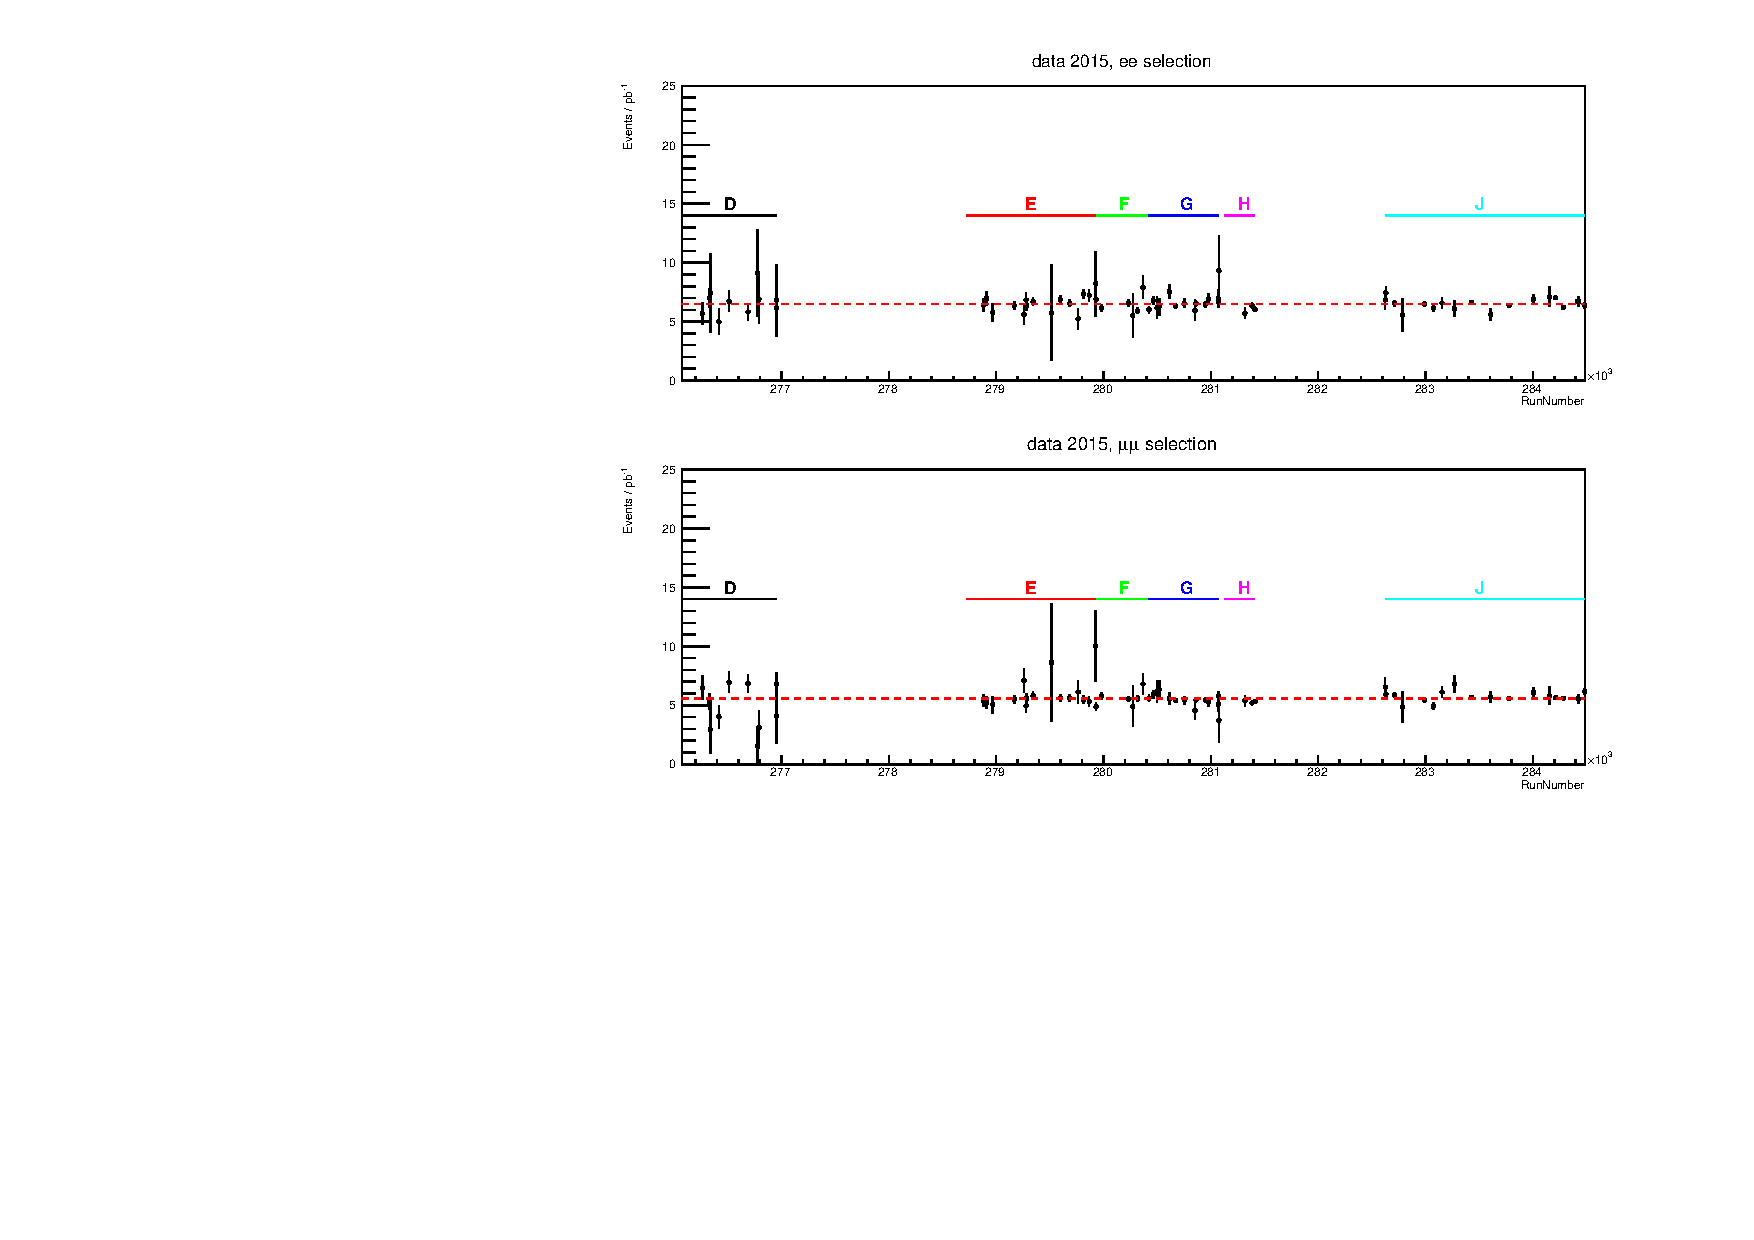
\includegraphics[width=\textwidth]{figures/analysis/datamc/Yields/compare_data_yields2015.pdf}
\caption[Data yields for the 2015 run period for the $ee$ (above) and $\mu\mu$ (below) selections.]{Data yields for the 2015 run period for the $ee$ (above) and $\mu\mu$ (below) selections. Each letter on the legend correspond to the different data taking periods within a year~\cite{Aad:2019fac}.}
\label{fig:yields2015}
\end{figure}

\begin{figure}[ht]
\centering
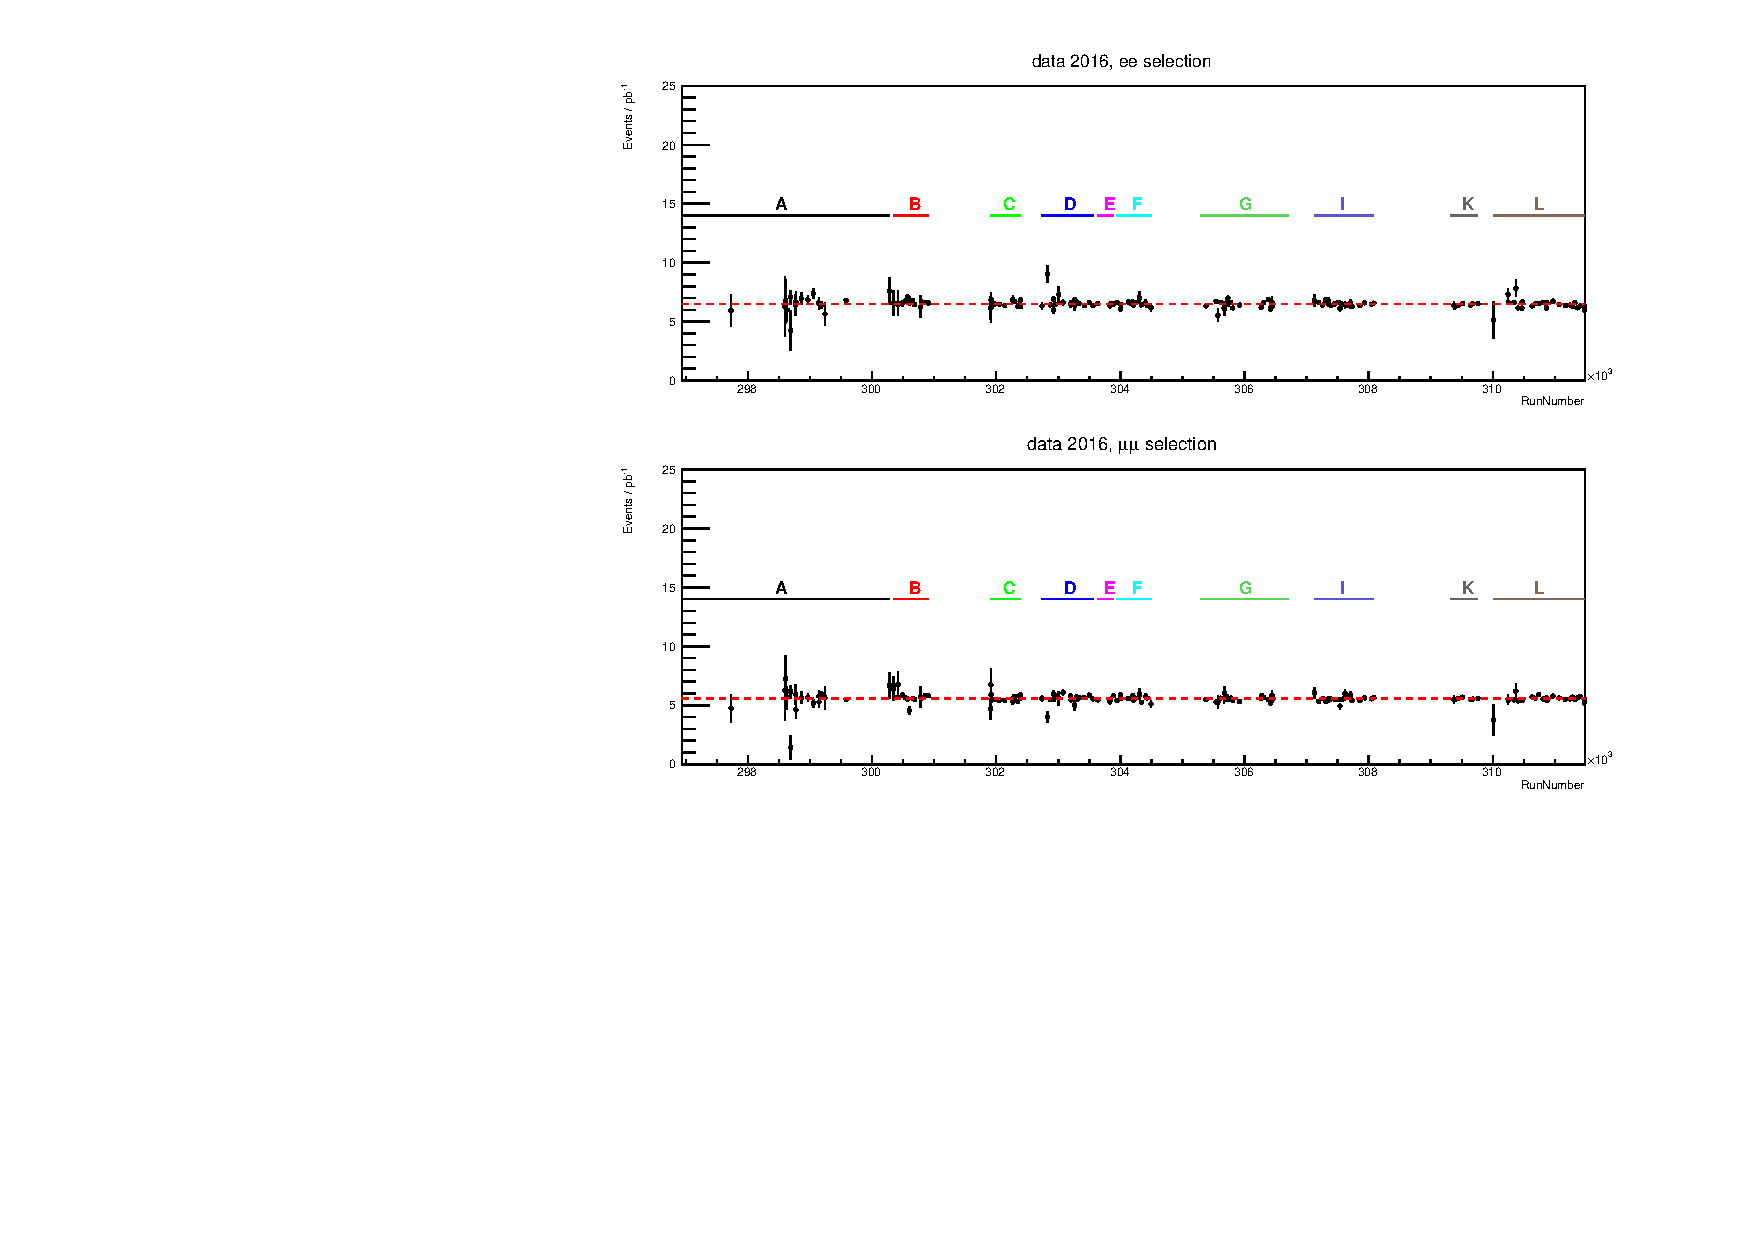
\includegraphics[width=\textwidth]{figures/analysis/datamc/Yields/compare_data_yields2016.pdf}
\caption[Data yields for the 2016 run period for the $ee$ (above) and $\mu\mu$ (below) selections.]{Data yields for the 2016 run period for the $ee$ (above) and $\mu\mu$ (below) selections. Each letter on the legend correspond to the different data taking periods within a year~\cite{Aad:2019fac}.}
\label{fig:yields2016}
\end{figure}

\begin{figure}[ht]
\centering
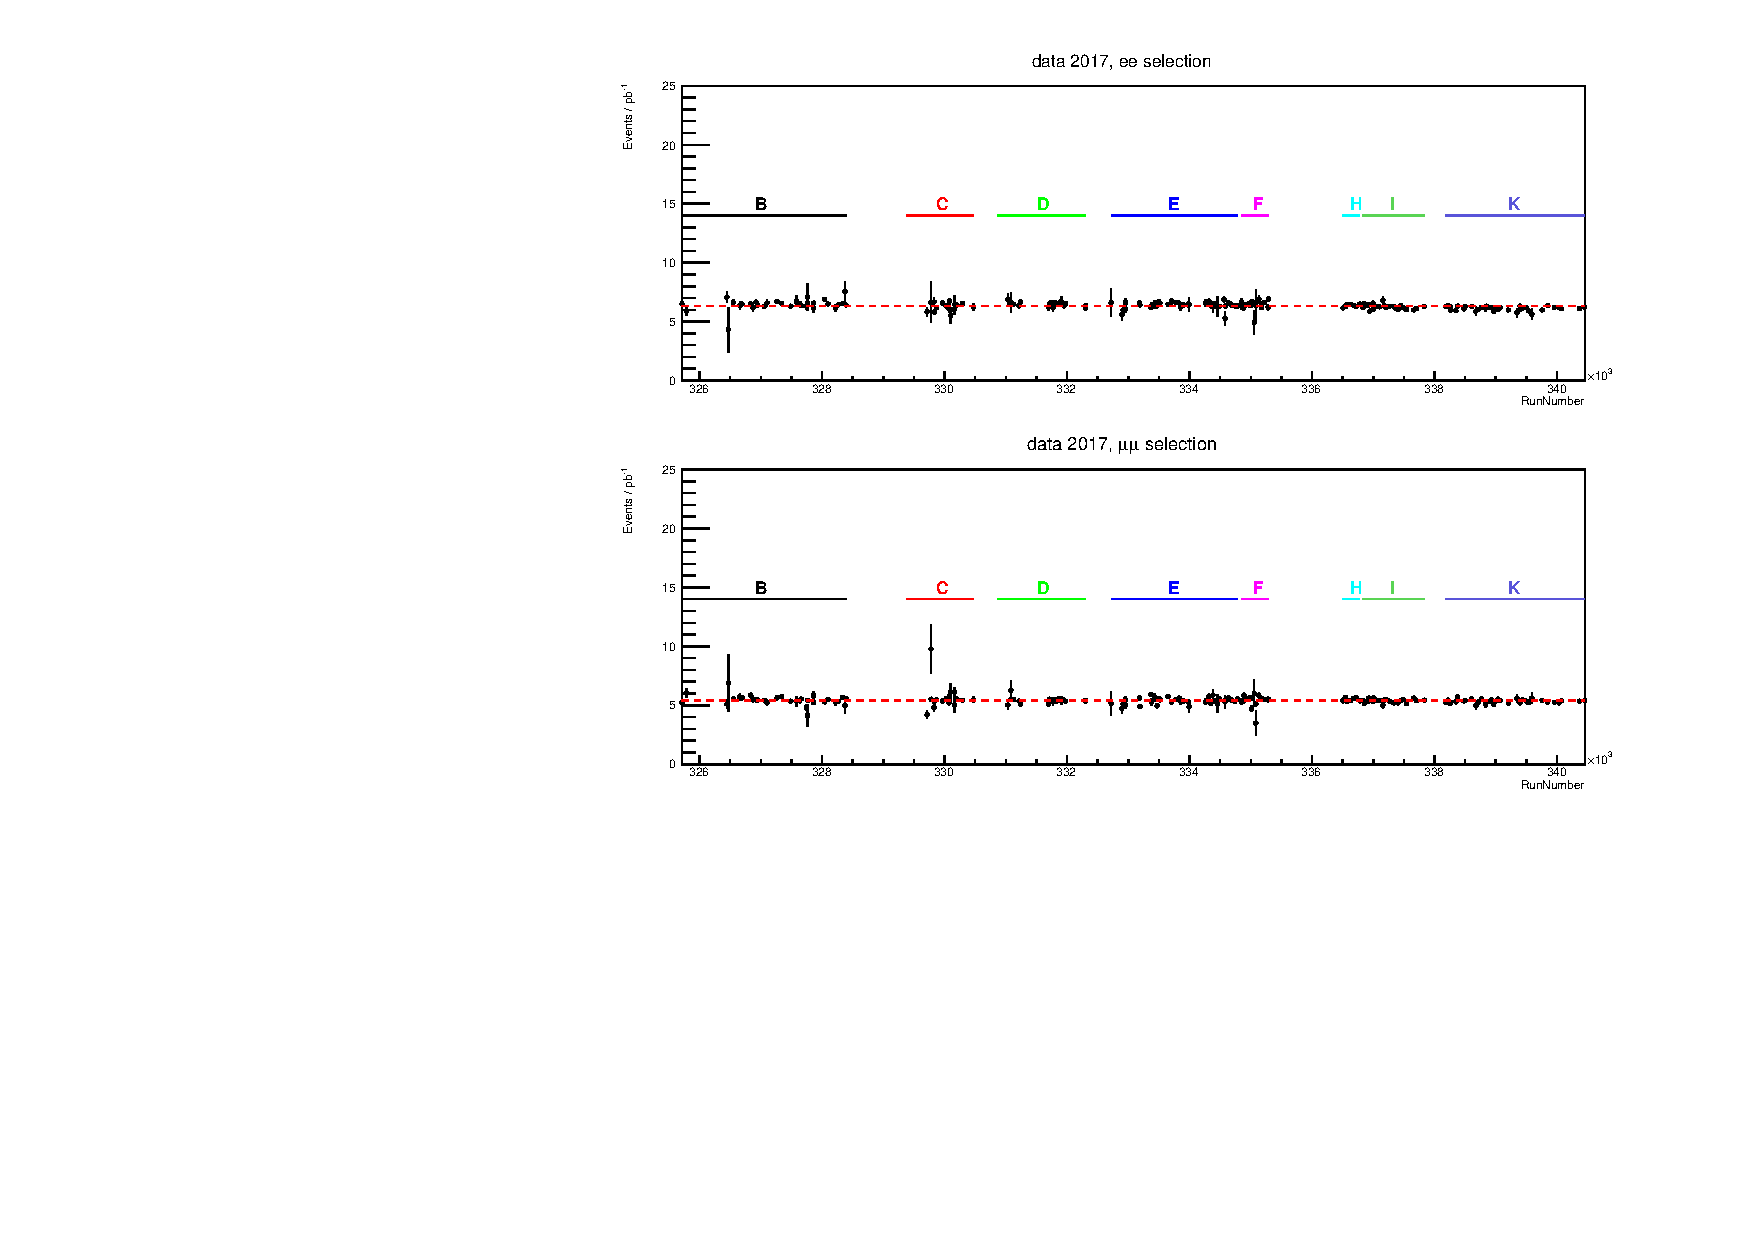
\includegraphics[width=\textwidth]{figures/analysis/datamc/Yields/compare_data_yields2017.pdf}
\caption[Data yields for the 2017 run period for the $ee$ (above) and $\mu\mu$ (below) selections.]{Data yields for the 2017 run period for the $ee$ (above) and $\mu\mu$ (below) selections. Each letter on the legend correspond to the different data taking periods within a year~\cite{Aad:2019fac}.}
\label{fig:yields2017}
\end{figure}

\begin{figure}[ht]
\centering
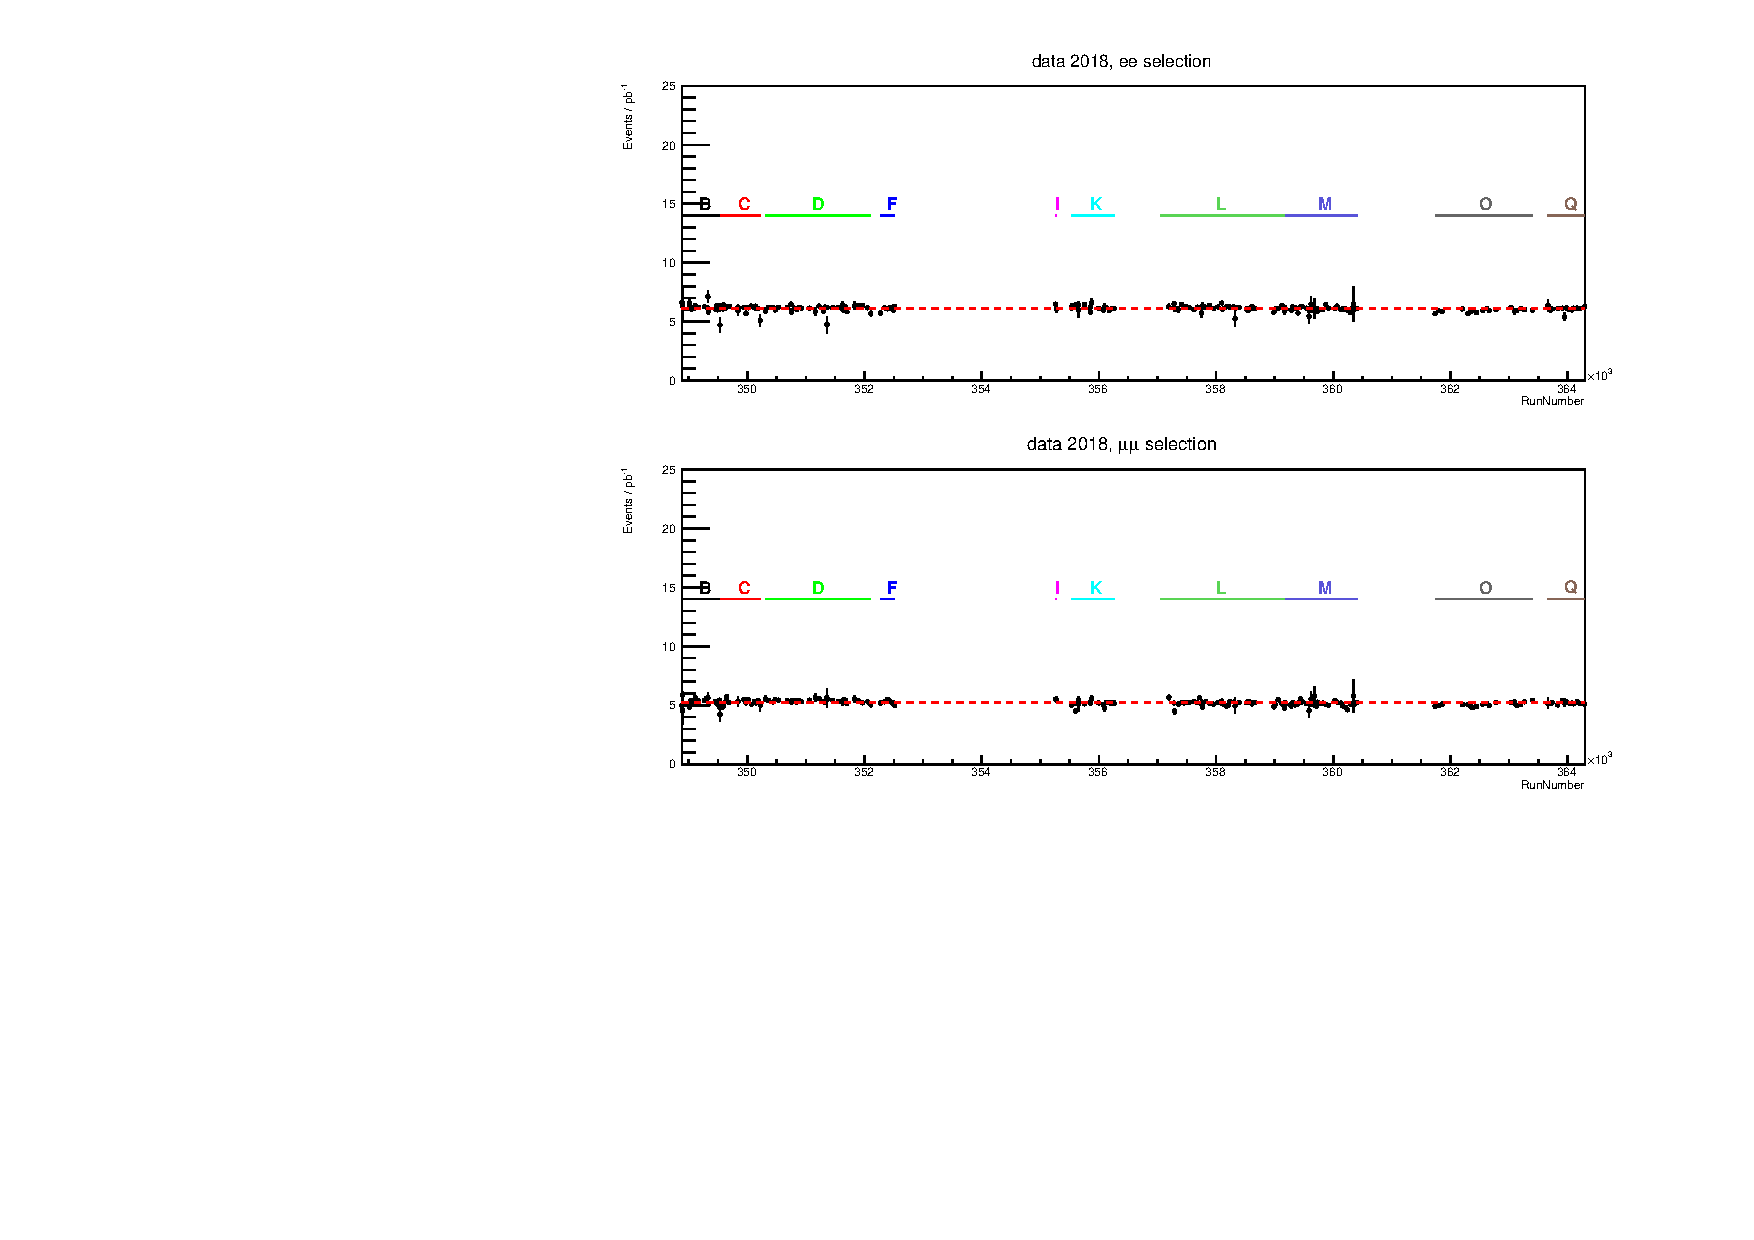
\includegraphics[width=\textwidth]{figures/analysis/datamc/Yields/compare_data_yields2018.pdf}
\caption[Data yields for the 2018 run period for the $ee$ (above) and $\mu\mu$ (below) selections.]{Data yields for the 2018 run period for the $ee$ (above) and $\mu\mu$ (below) selections Each letter on the legend correspond to the different data taking periods within a year~\cite{Aad:2019fac}.}
\label{fig:yields2018}
\end{figure}

\clearpage

\section{Monte Carlo samples}\label{sec:datamc:mc}
Whilst the analysis is performed using a data-driven methodology, simulated samples for the background and signal are used to determine the appropriate functional form to fit the data, study background compositions, estimate uncertainties and evaluate the expected signal contribution in the signal regions. This section outlines the MC samples used for the background and signal samples.

There are generators used to produce events using higher-order matrix elements. However, it is often required to enhance the description of the process beyond the order of the generator used. Higher-order QCD and EW corrections can modify the shape of the invariant mass distributions. Mass-dependent \emph{K}-factors are derived from taking the ratio of the higher-order differential cross-section calculation over the available sample, e.g. next-to-next-to-leading order (NNLO) over the next-to-leading order (NLO). The \emph{K}-factors are then applied to the invariant mass distribution on an event by event basis to produce the higher-order samples. 

Simulated samples include the effects of pileup interactions, performed with \PYTHIAV{v8.186} using the ATLAS A3 set of tuned parameters~\cite{ATL-PHYS-PUB-2016-017} and the NNPDF23LO PDF set, and weighted accordingly to the number of pileup interactions observed in data. The simulated samples then pass through the full detector simulation as described in \cref{sec:simulation}. 

\subsection{Background samples}\label{sec:datamc:mc:bkg}
The main backgrounds considered in the analysis, in decreasing order of importance, are Drell-Yan (DY), top-quark ($t\bar{t}$), single-top-quark and diboson production. For the electron channel, is it prohibitive to produce MC with enough events to accurately represent the expected QCD multijet distribution, due to the small probability of jets faking electrons that pass the analysis selection. Therefore, the QCD and $W$+Jets processes in the dielectron channel are estimated with a data-driven method~\cite{EXOT-2016-05}, described in \cref{sec:datamc:fakes}. For the muon channel, the multijet background was studied and found to be negligible~\cite{EXOT-2016-05}. Therefore, the contribution is neglected. 

The SM Drell-Yan process is modelled using the NLO \POWHEGBOX~\cite{Alioli:2010xd,Frixione:2007vw} event generator using the CT10 PDF~\cite{ct10} and is interfaced with \PYTHIAV{v8.186}~\cite{pythia8} parton shower generator. The DY samples are generated in slices of dilepton invariant mass, where 19 mass-binned samples were created with dilepton invariant mass ranging from \SI{120}{\giga\electronvolt} and $>$ \SI{5000}{\giga\electronvolt}, to increase the statistics of the samples in the high-mass regions. Corrections are applied to the DY samples to correct them from NLO to NNLO using a mass-dependent \emph{K}-factor. The \emph{K}-factor calculated with {\textsc{VRAP}} v0.9~\cite{vrap} and the CT14 NNLO PDF set~\cite{CT14} for QCD effects. {\textsc{MCSANC}}~\cite{MCSANC} is used for QED corrections. The diboson processes ($WW$, $WZ$ and $ZZ$) are generated at NLO using \SHERPA 2.1.1~\cite{Gleisberg:2008ta} with the CT10 PDF. Similar to the DY samples, the diboson samples were generated in invariant mass slices to increase the statistics of the sample. The $t\bar{t}$ background is generated at NLO using \POWHEGBOX with the NNPDF3.0NLO~\cite{Ball:2014uwa} PDF. Single top (s/t-channel) uses \POWHEGBOX with NNPDF3.0NLO PDF. A top quark mass of \SI{172.5}{\giga\electronvolt} is used for the generation of these samples. The top quark samples are normalised to the cross-section at NNLO in QCD including resummation of the NNLO leading order soft gluon terms as provided by \textsc{Top++}2.0~\cite{Czakon:2011xx}.

The MC event generators for the hard-scattering process, showering and PDFs are listed in \cref{tab:MC}. A detailed description of the event simulation procedure is given in \cref{sec:simulation}. "Afterburner" generators such as \textsc{Photos}~\cite{Golonka:2005pn} for the final-state photon radiation (FSR) modelling, \textsc{MadSpin}~\cite{Artoisenet:2012st} to preserve top-quark spin correlations, and \textsc{EvtGen}~\cite{Lange:2001uf}, used for the modelling of $c$- and $b$-hadron decays, are also included in the simulation.

\begin{table}[htbp]
\centering
\tablesize{
\begin{tabular}{llp{5cm}}
\toprule
Background Process & ME Generator and ME PDFs & PS and non-perturbative effect with PDFs \\\hline
NLO Drell--Yan & \POWHEGBOX~\cite{Alioli:2010xd,Frixione:2007vw}, CT10~\cite{ct10}, \textsc{Photos} & \PYTHIAV{v8.186}~\cite{pythia8}, CTEQ6L1~\cite{ATL-PHYS-PUB-2014-021,Stump:2003yu}, \newline \textsc{EvtGen1.2.0} \\
$t\bar{t}$  & \POWHEGBOX, NNPDF3.0NLO~\cite{Ball:2014uwa} & \PYTHIAV{v8.230}, NNPDF23LO~\cite{Ball:2012cx}, \newline \textsc{EvtGen1.6.0} \\
Single top $s$-channel, $Wt$& \POWHEGBOX, NNPDF3.0NLO & \PYTHIAV{v8.230}, NNPDF23LO, \newline \textsc{EvtGen1.6.0} \\
Single top $t$-channel & \POWHEGBOX, NNPDF3.04fNLO, \textsc{MadSpin} & \PYTHIAV{v8.230}, NNPDF23LO,\newline  \textsc{EvtGen1.6.0}  \\
Diboson ($WW$, $WZ$ and $ZZ$) & \SHERPA 2.1.1~\cite{Gleisberg:2008ta}, CT10 &\SHERPA 2.1.1, CT10  \\\hline
Signal Process & & \\\hline
LO Drell--Yan & \PYTHIAV{v8.186}, NNPDF23LO  &  \PYTHIAV{v8.186}, NNPDF23LO, \newline \textsc{EvtGen1.2.0} \\
LO CI & \PYTHIAV{v8.186}, NNPDF23LO  &  \PYTHIAV{v8.186}, NNPDF23LO, \newline \textsc{EvtGen1.2.0} \\
\bottomrule
\end{tabular}
}
\caption[The event generators used for PDFs and generating matrix element (ME) and parton shower (PS) simulation of the signal and background processes.]{The event generators used for PDFs and generating matrix element (ME) and parton shower (PS) simulation of the signal and background processes. The top-quark mass is set to \SI{172.5}{\giga\electronvolt}.}
\label{tab:MC}
\end{table}

\subsection{Signal samples}\label{sec:datamc:mc:sig}
The \PYTHIAV{v8.230} generator is used to produce CI signal samples at leading-order (LO) using the NNPDF23LO PDF. Five benchmark values of $\Lambda$ from 10-\SI{30}{\tera\electronvolt} in steps of \SI{5}{\tera\electronvolt} were generated for each of the CI models. The CI shapes contain both the SM DY background and the interference between the DY and CI. 

It is possible to reweight the SM background to BSM signals when both the signal and background have the same initial and final states. Event-by-event weights are calculated and applied to the DY events passing the event selection, resulting in the DY sample being \emph{reweighted} into corresponding CI signal events. This allows the production of unique samples of CI signal events, which match the signal samples produced using MC, but with a significant reduction in the computing power required~\cite{EXOT-2016-05}. 

The signal templates include the same set of experimental and theoretical corrections as applied with other samples described in \cref{sec:datamc:mc}. In addition, higher order QCD and EW corrections are also applied, resulting in the same LO-to-NNLO mass-dependent \emph{k}-factors as the background MC. While higher-order QCD corrections are expected to be the same for signals and background, it is not clear if the electroweak corrections can be treated the same. The addition of the electroweak corrections may be less conservative. However, it is deemed to be closer to the theoretically correct treatment than being over conservative and not including the corrections. 

Signal templates are produced from the reweighting of the \PYTHIAV{v8.186} LO DY simulation. The general procedure is to replace the DY differential cross-section with the corresponding cross-section of the CI process, where
\begin{equation}
   \frac{d\sigma}{d\hat{t}}(q\bar{q} \rightarrow \gamma^*/Z \rightarrow \ee) \rightarrow \frac{d\sigma}{d\hat{t}}(q\bar{q} \rightarrow CI \rightarrow \ee),
\end{equation}
where $\hat{t}$ corresponds to any kinematic quantity. The above can be achieved using the analytic expressions for the DY and CI matrix elements. The ratio between the two matrix elements, evaluated with the truth-level kinematic information of the dielectron and dimuon events, defines the weight, $w_{\mathrm{RW}}$, used to reweight the DY event to the corresponding CI event. The weight is given by~\cite{EXOT-2016-05}
\begin{equation}
    w_{\mathrm{RW}} = |\mathcal{M}(CI)|^2~/~|\mathcal{M}(\gamma^*/Z)|^2~,
\end{equation}
where the numerator refers to the BSM differential cross-section and the denominator refers to the SM process only. The weights are applied to the LO DY events to transform into CI signal shapes, in steps of \SI{2}{\tera\electronvolt} between $\Lambda = \SI{12}{\tera\electronvolt}$ and $\Lambda = \SI{100}{\tera\electronvolt}$. 

The dedicated CI samples are used to validate the reweighting procedure, \cref{fig:datamc:sigValidate} shows an example of a LL chiral, constructive interference, CI mass slice between 3000 - \SI{4000}{\giga\electronvolt} where the reweighted CI interaction sample and the dedicated sample is compared. \cref{fig:datamc:sigoverlays} shows the invariant mass distributions for the LL chiral constructive and destructive interference models reweighted using the procedure described above. \cref{fig:datamc:sigShape} depicts the shapes of the LL chiral CI interaction signals relative to the DY background These depict the evolution of the shapes as the interference and $\Lambda$ of the CI models change. The CI samples include the full cross-section (including the DY component) as defined in \cref{sec:bsm:ci}.

\begin{figure}[h]
    \centering
    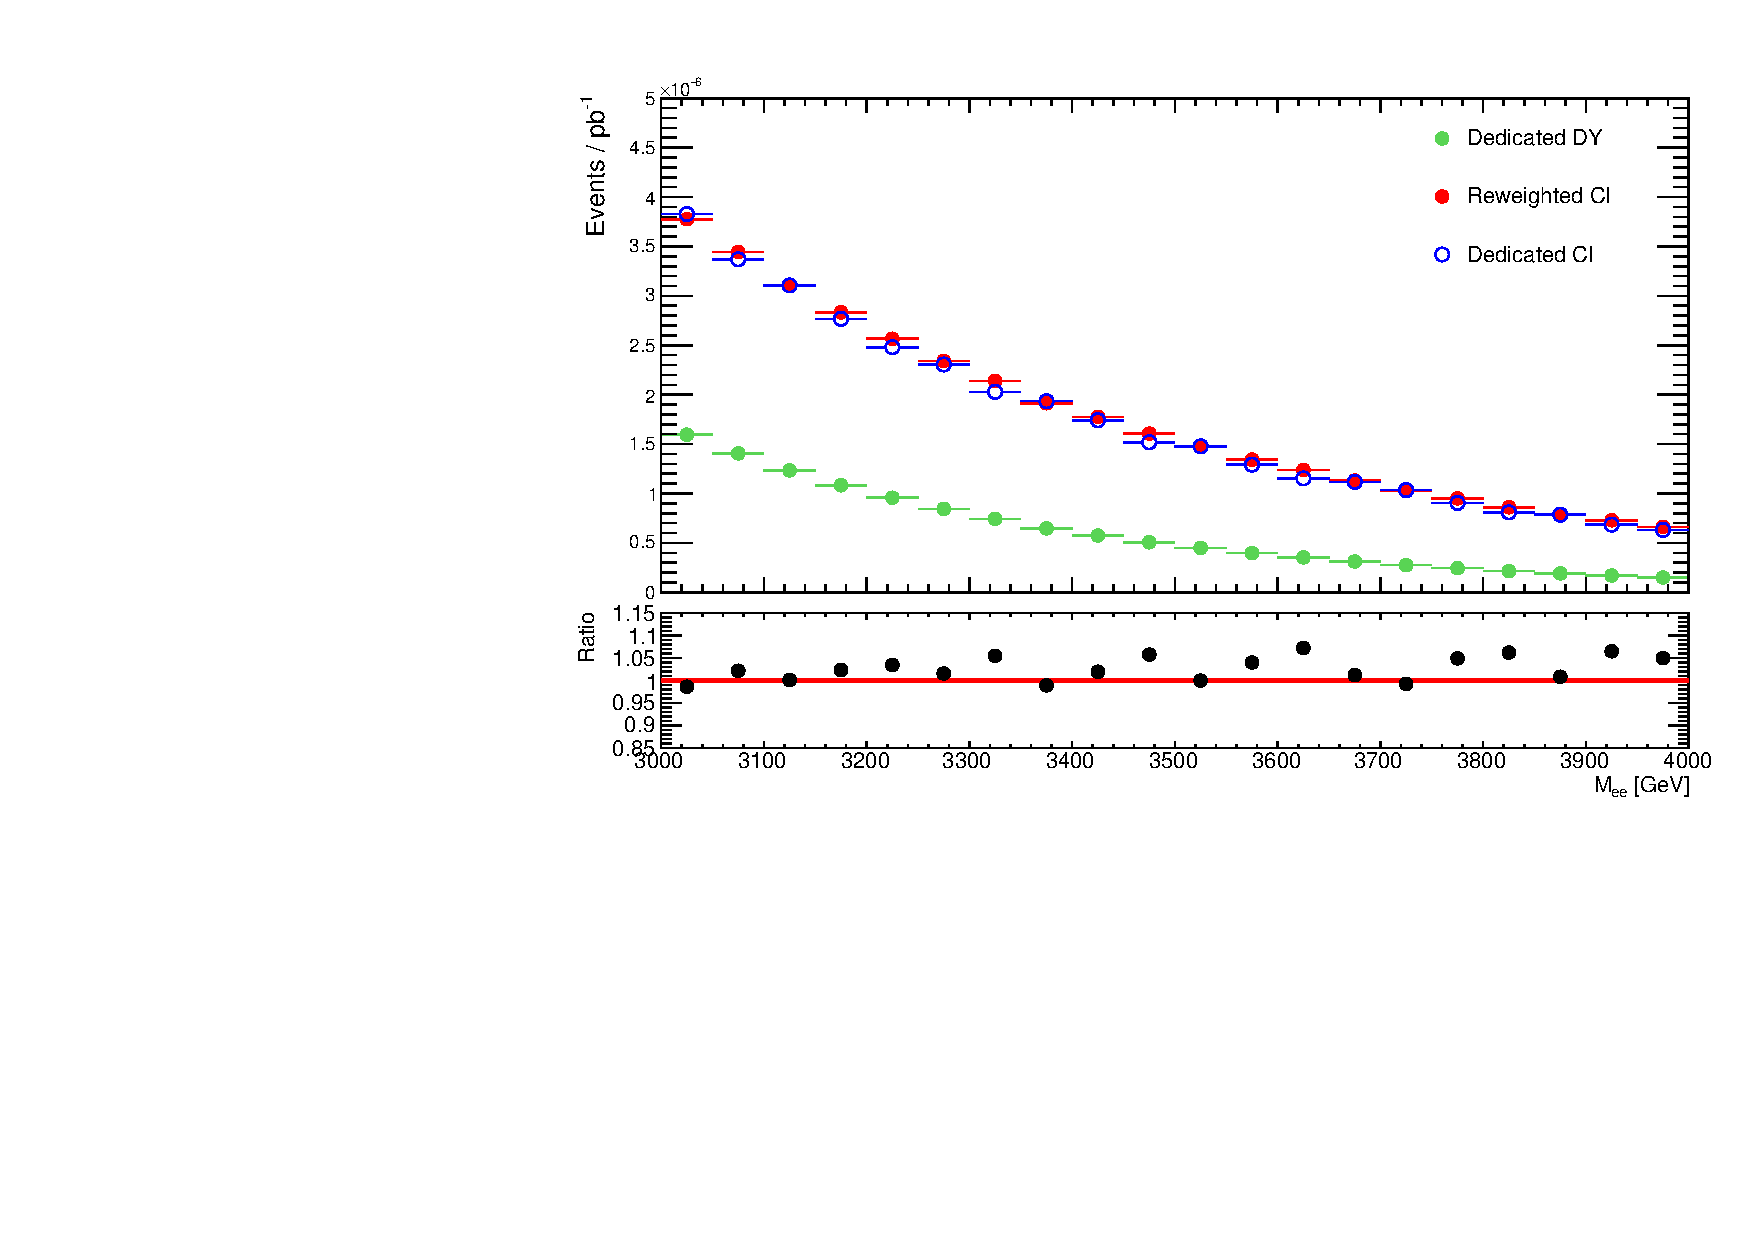
\includegraphics[width=\mediumfigwidth]{figures/analysis/datamc/sigmodel/CICompare.pdf}
    \caption[Validation of signal reweighting]{Comparison of dedicated and reweighted LL chiral, constructive interference, CI sample in the invariant mass range from 3000 - \SI{4000}{\giga\electronvolt} is shown in the top pad. The DY sample used to reweight is also shown. The bottom pad shows the ratio between the reweighted and dedicated CI signal.}
    \label{fig:datamc:sigValidate}
\end{figure}

\begin{figure}[]
    \centering
    \begin{subfigure}[b]{0.49\textwidth}
        \centering
        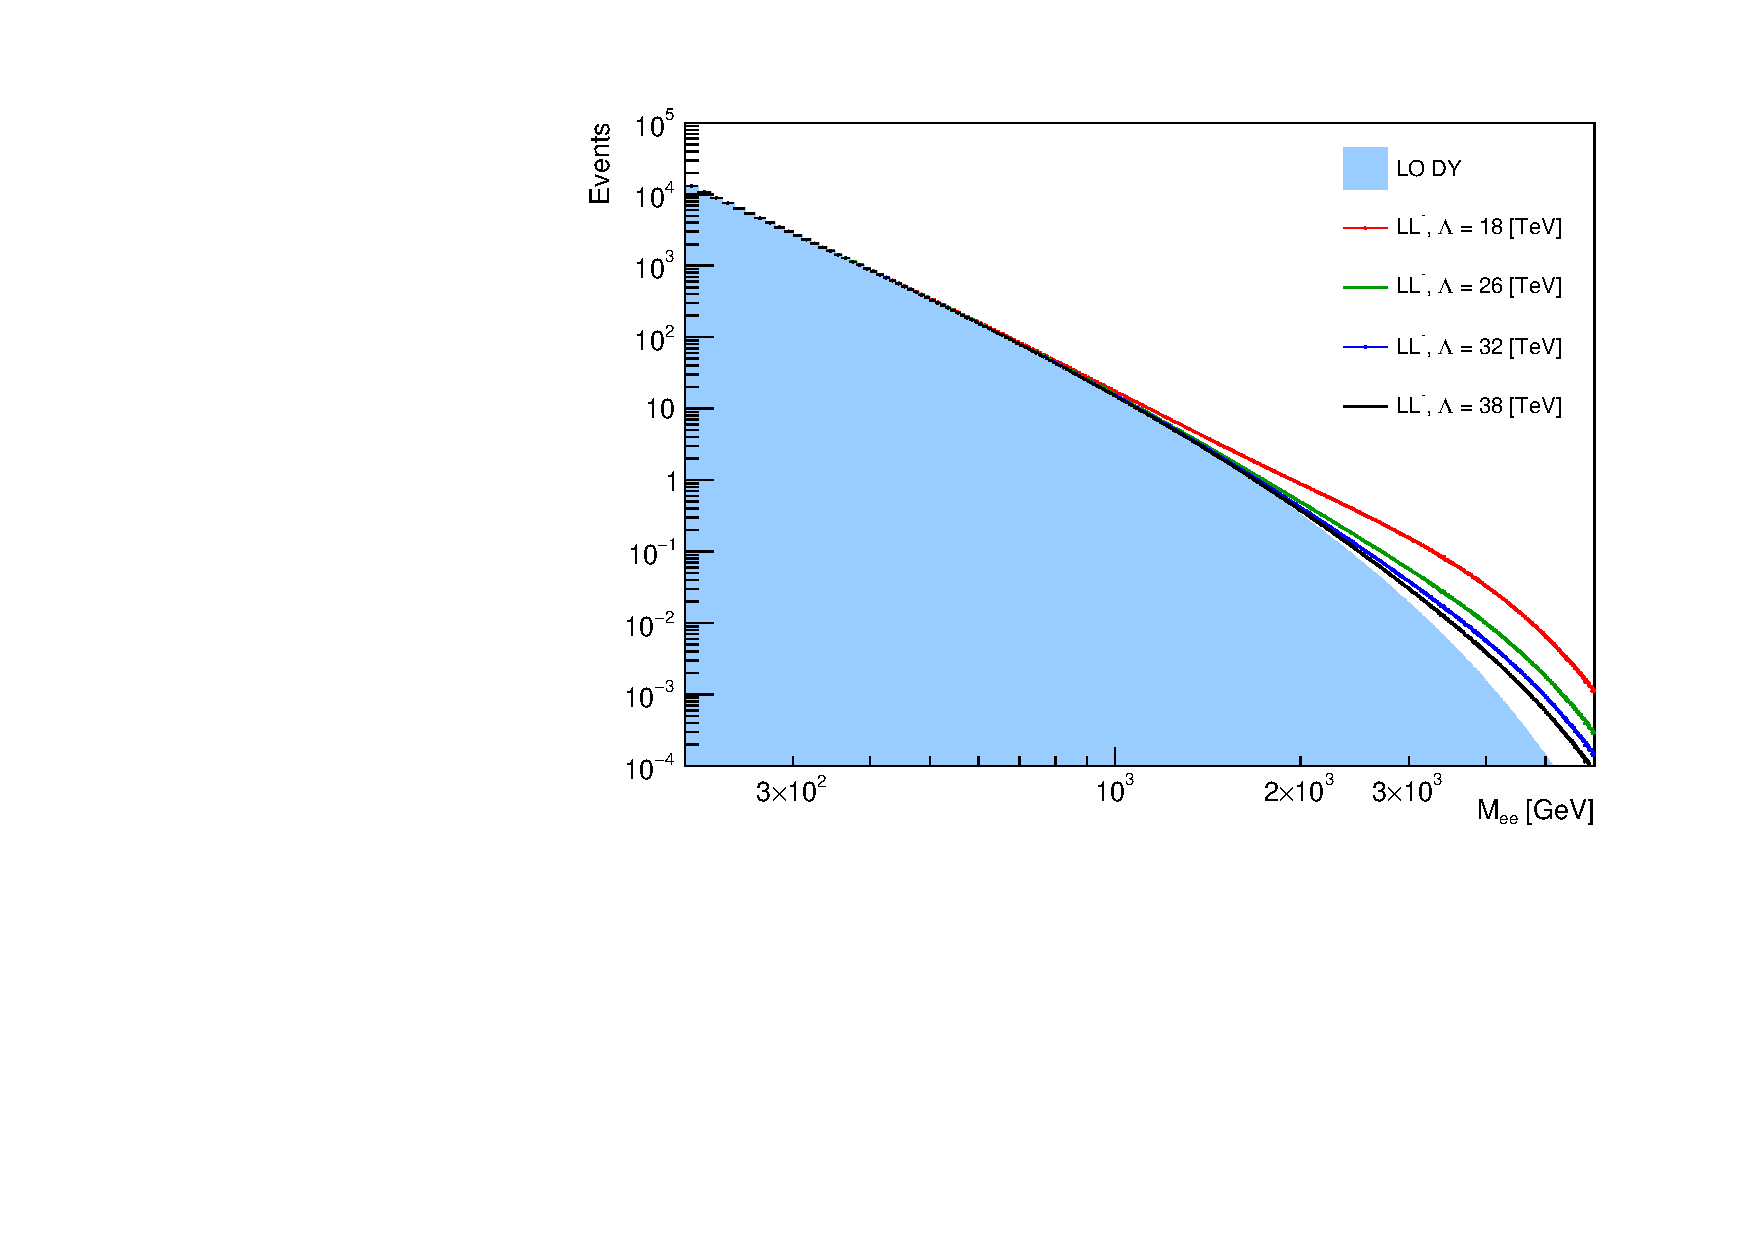
\includegraphics[width=\textwidth]{figures/analysis/datamc/sigmodel/constSigsOverlay.pdf}
        \label{fig:datamc:sigconstoverlays}
    \end{subfigure}
    \begin{subfigure}[b]{0.49\textwidth}
        \centering
        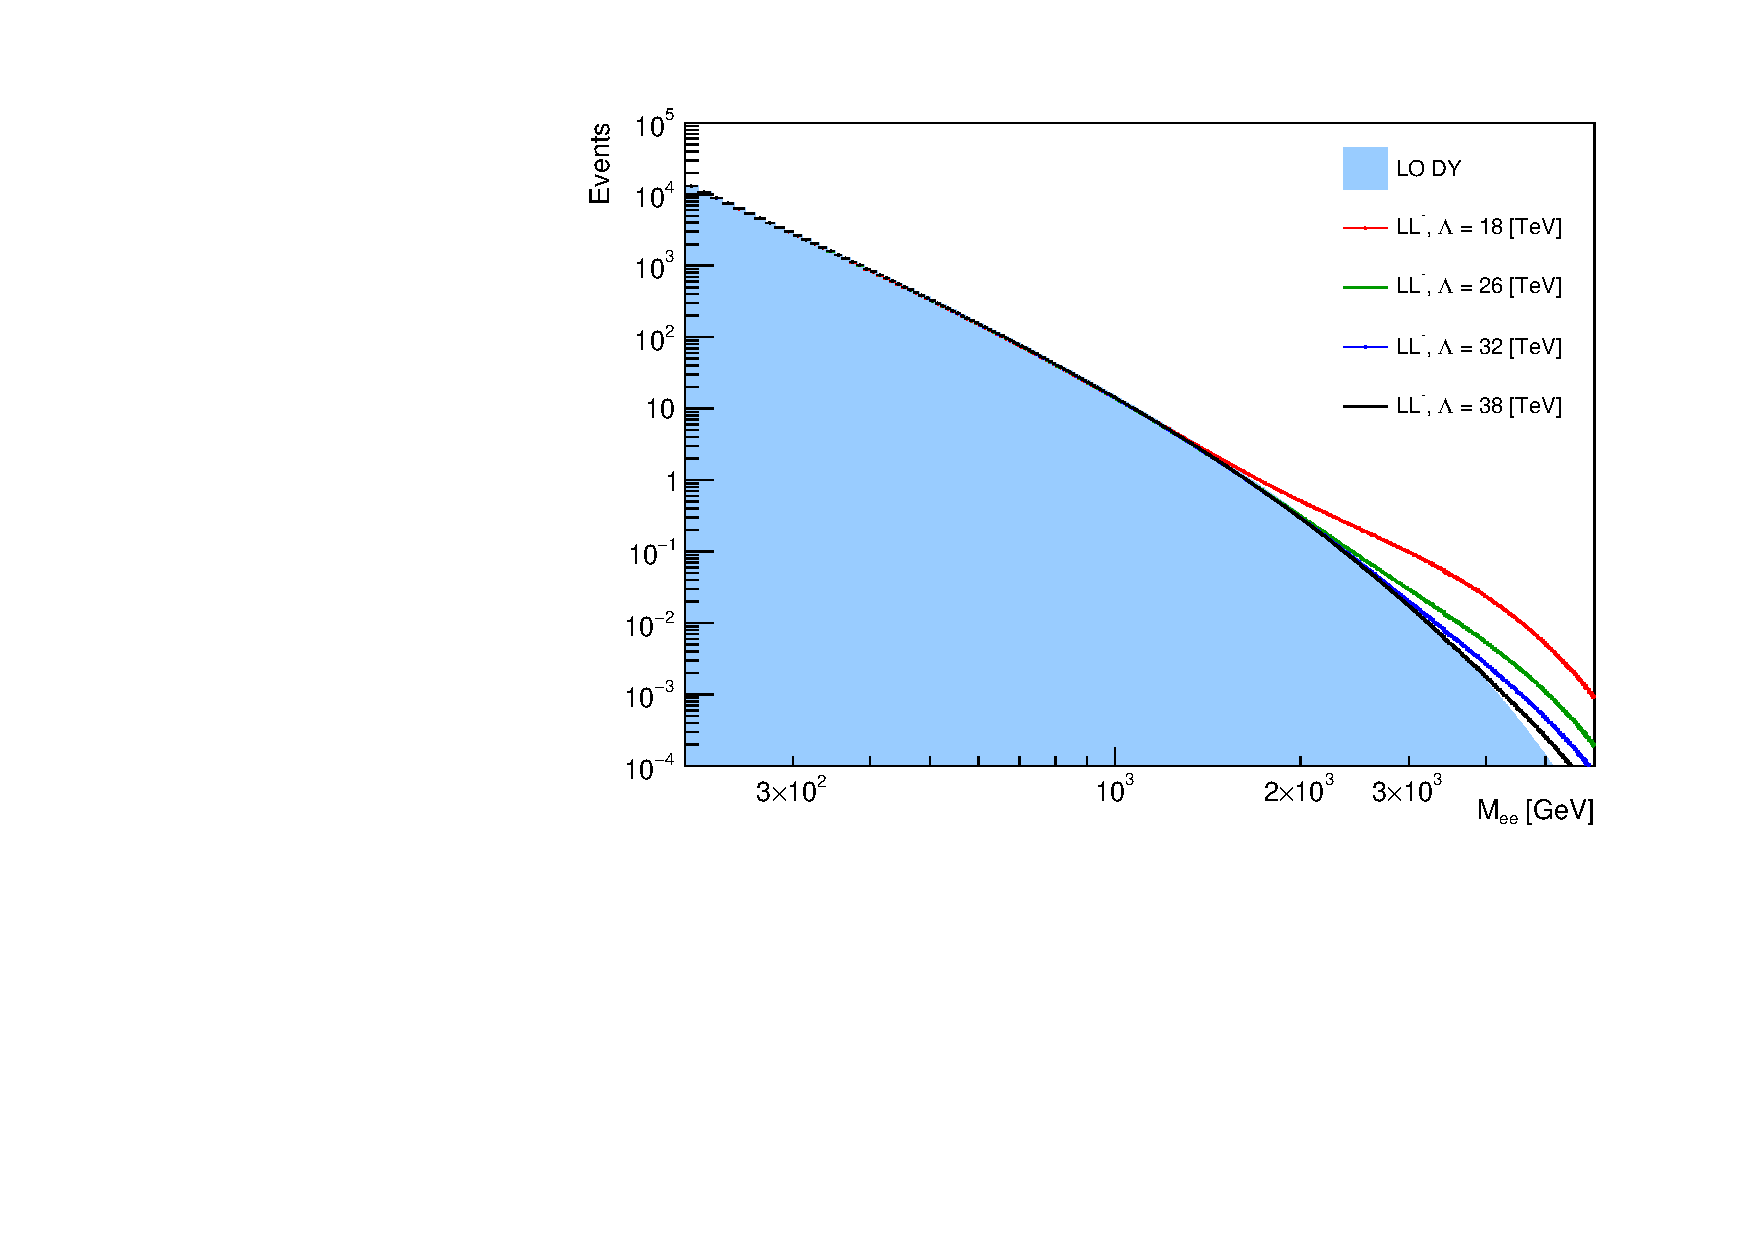
\includegraphics[width=\textwidth]{figures/analysis/datamc/sigmodel/destSigsOverlay.pdf}
        \label{fig:datamc:sigdestoverlays}
    \end{subfigure}
    \caption[Invariant mass distribution for reweighted CI LL chiral signal models]{Invariant mass distributions for LL chiral, constructive (left) and destructive (right) interference CI models with the DY sample used to reweight it. The interference of the CI interaction is shown by the - (constructive) and + (destructive) sign on the legend.}
    \label{fig:datamc:sigoverlays}
\end{figure}

\begin{figure}[]
    \centering
    \begin{subfigure}[b]{0.49\textwidth}
        \centering
        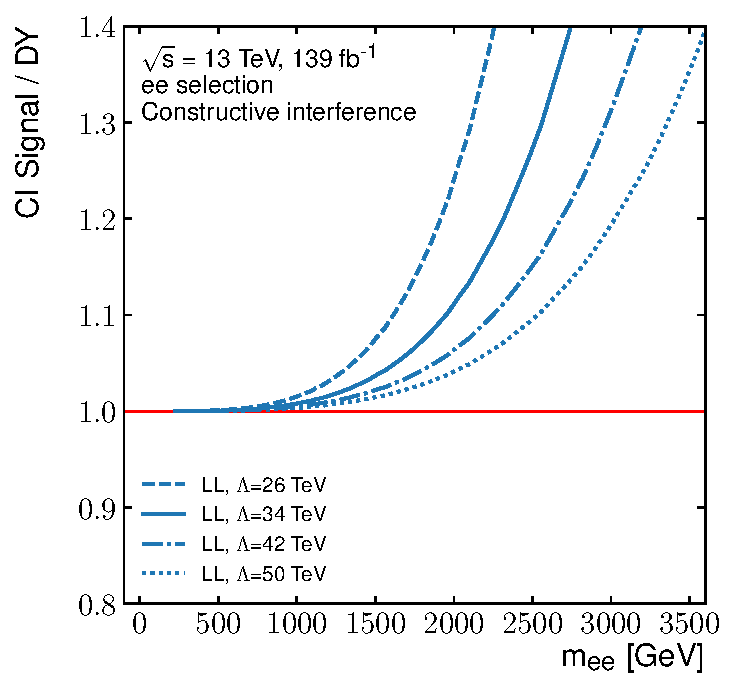
\includegraphics[width=\textwidth]{figures/analysis/datamc/sigmodel/fit-const-ee-backgroundModel.pdf}
    
        \label{fig:datamc:sigShape1}
    \end{subfigure}
    \begin{subfigure}[b]{0.49\textwidth}
        \centering
        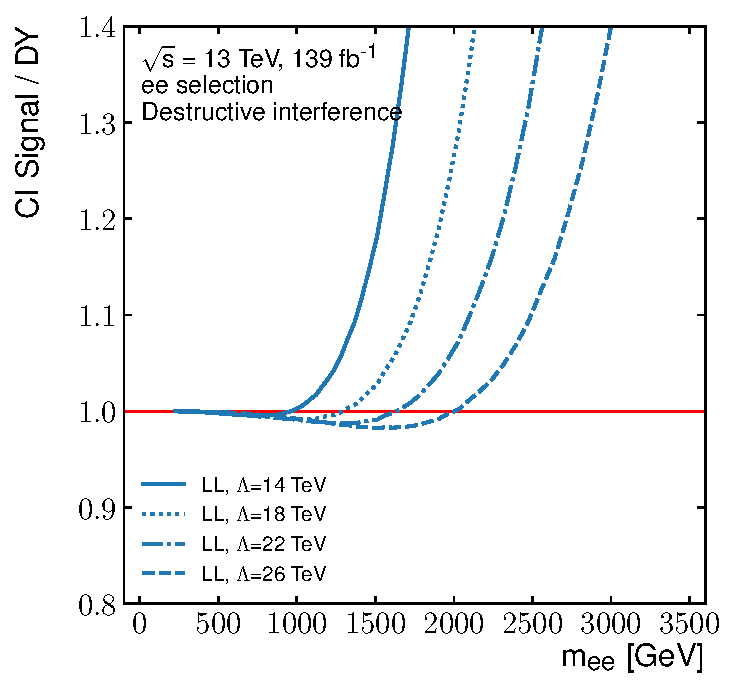
\includegraphics[width=\textwidth]{figures/analysis/datamc/sigmodel/fit-dest-ee-backgroundModel.pdf}
    
        \label{fig:datamc:sigShape2}
    \end{subfigure}
    \begin{subfigure}[b]{0.49\textwidth}
        \centering
        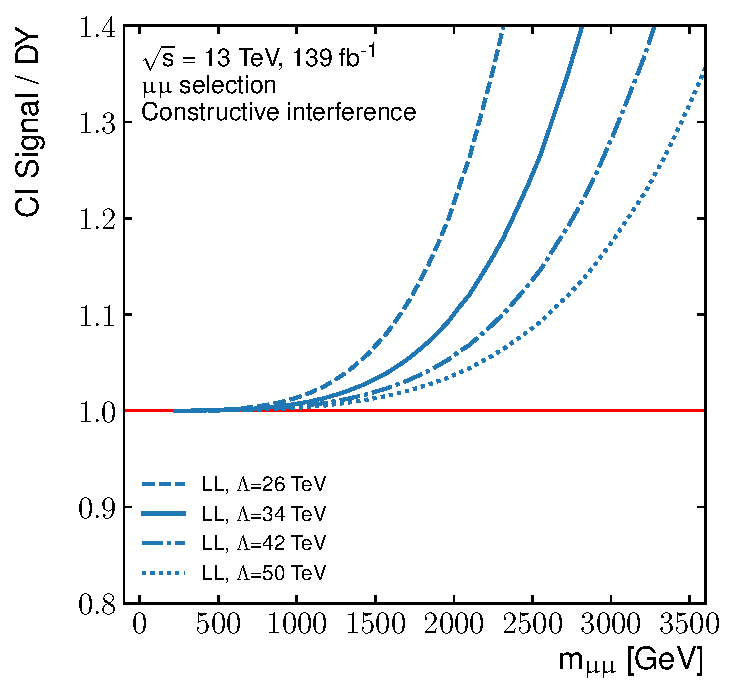
\includegraphics[width=\textwidth]{figures/analysis/datamc/sigmodel/fit-const-mm-backgroundModel.pdf}
    
        \label{fig:datamc:sigShape3}
    \end{subfigure}
    \begin{subfigure}[b]{0.49\textwidth}
        \centering
        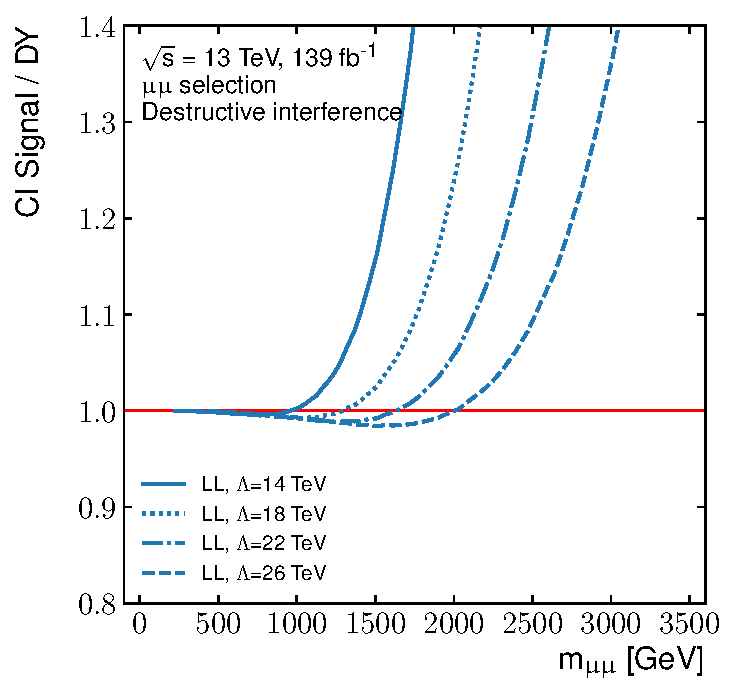
\includegraphics[width=\textwidth]{figures/analysis/datamc/sigmodel/fit-dest-mm-backgroundModel.pdf}
    
        \label{fig:datamc:sigShape4}
    \end{subfigure}
    \caption[The ratio of the contact interaction signal shape added to the Drell-Yan background (signal+DY) background to the Drell-Yan background is shown for various contact interaction scales, $\Lambda$.]{The ratio of the contact interaction signal with the DY background is shown for various contact interaction scales, $\Lambda$. For constructive cases, the ratio is purely positive, while for destructive cases the impact of destructive interference is seen at lower masses. Shown from left to right and top to bottom, \ee constructive, \ee destructive, \mumu constructive, and \mumu destructive.}
    \label{fig:datamc:sigShape}
\end{figure}

\subsubsection{Signal template morphing}\label{sec:datamc:mc:sig:morphing}
The CI samples are produced in steps of \SI{2}{\tera\electronvolt} from 12-\SI{100} {\tera\electronvolt} using the reweighting procedure outlined in \cref{sec:datamc:mc:sig}. The DY component is subtracted from the simulated signals, leaving the pure CI and interference terms. The signal model used in the analysis (\cref{sec:sigmodel}) requires a continuous description of the signal model as a function of $\Lambda$ to fit possible signal contributions that may be between the reweighted signal masses. To implement the signal template morphing a custom signal probability distribution class was created derived from two available RooFit~\cite{RooFit}. A linear interpolation is used to provide a smoothly changing PDF that is dependent on the parameter $\Lambda$.  
% classes: a class to model the shape of the signal as a function of $\Lambda$ and another to model the normalisation of the signal as a function of $\Lambda$. There are several classes within RooFit to perform morphing between histograms. However, an advantage of the custom PDF class is that it allows for integration into the existing framework created for the background estimation and statistical analysis. The parameter $\Lambda$ can be easily adjusted to provide a smoothly changing PDF and normalisation.
\cref{fig:bkgmodel:Morph} depicts the morphed signal PDF for various values of $\Lambda$ for constructive and destructive CI interference models. It shows the morphed signals for the LL chirality model, but, the signal PDFs are produced for all chirality models considered in the analysis. For constructive models, the shape of the signal does not change significantly as a function of $\Lambda$. However, for the destructive models, a strong relationship between the shape of the signal and $\Lambda$ can be seen. The downward \emph{dip} in the destructive plots corresponds to the point at which the destructive interference is dominant and hence where a negative signal yield is expected. \cref{fig:bkgmodel:ratioMorph} shows the comparison of a CI template for $\Lambda = \SI{20}{\tera\electronvolt}$ compared with the corresponding morphed signal template, and a good agreement between the two is shown in the ratio panel. Statistical fluctuations in the reweighted samples result in small differences between the morphed and reweighted templates. 

Furthermore, the morphed signal PDFs can be used in the statistical analysis to describe the signal model. For the search of non-resonant signals like CI, it is prohibitive to describe the signal model with a floating signal strength parameter, $\mu$. When searching for resonances, it is natural to use $\mu$ as the parameter of interest, which describes the strength of the signal. However, due to the shape and normalisation changes of the signal models as a function of $\Lambda$, it is more accurate to define the parameter of interest as a function of $\Lambda$. Further details of the statistical analysis and choice of the parameter of interest is given in \cref{sec:stat:poi}

\begin{figure}[h!]
    \centering
    \begin{subfigure}[b]{0.49\textwidth}
        \centering
        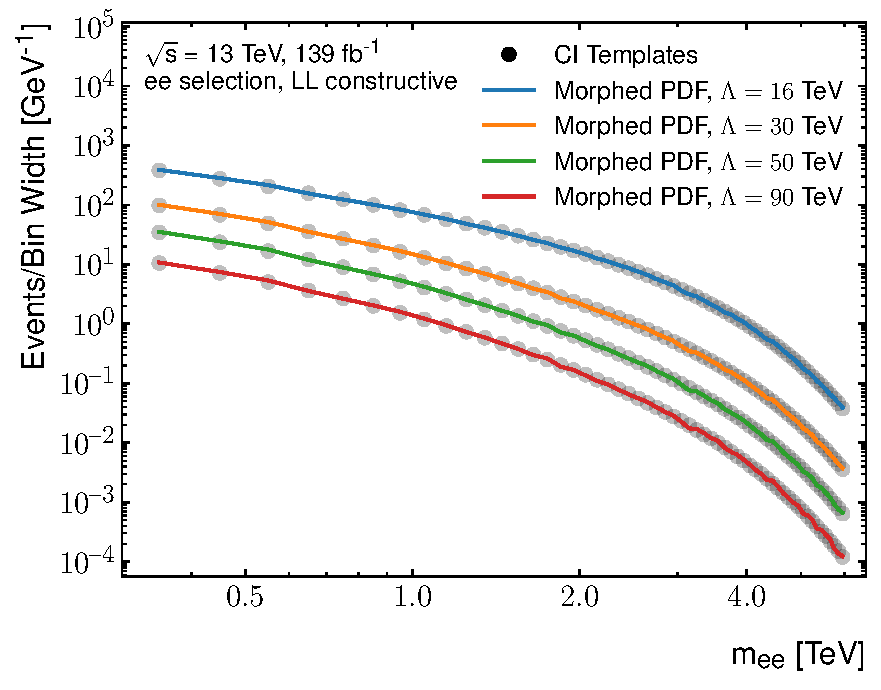
\includegraphics[width=\textwidth]{/Users/Deshan/Documents/PhD/thesis/Thesis/figures/analysis/bkgmodel/sigComp-const-LL-ee.pdf}
        \label{fig:bkgmodel:Morphee1}
    \end{subfigure}
    \begin{subfigure}[b]{0.49\textwidth}
        \centering
        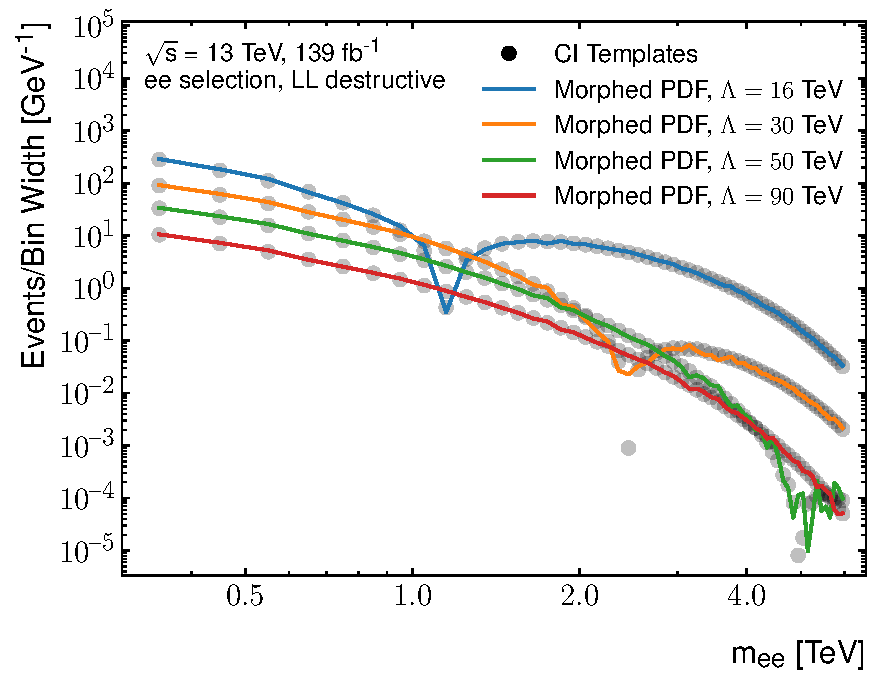
\includegraphics[width=\textwidth]{/Users/Deshan/Documents/PhD/thesis/Thesis/figures/analysis/bkgmodel/sigComp-dest-LL-ee.pdf}
        \label{fig:bkgmodel:Morphee2}
    \end{subfigure}
    \begin{subfigure}[b]{0.49\textwidth}
        \centering
        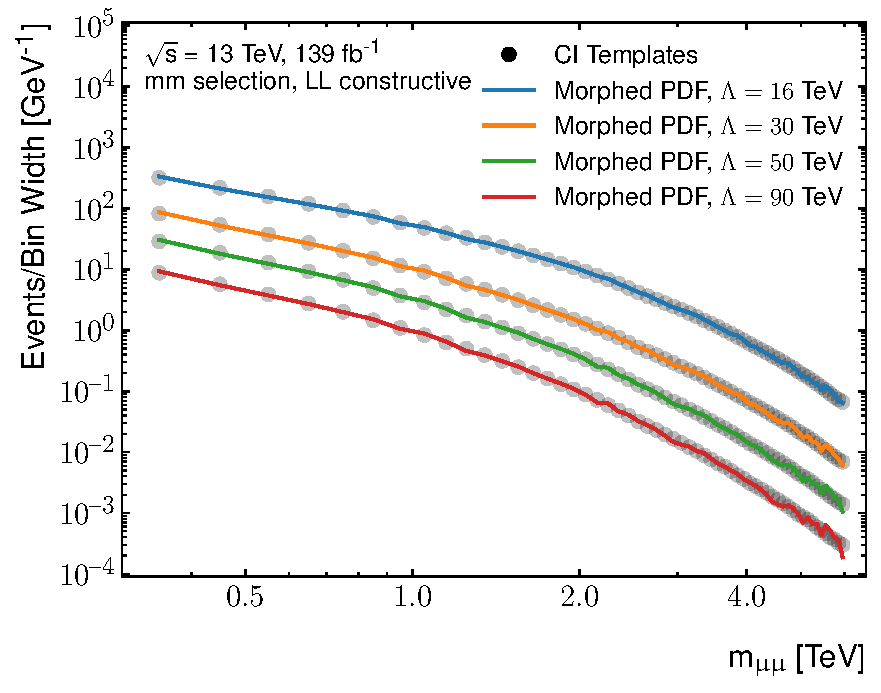
\includegraphics[width=\textwidth]{/Users/Deshan/Documents/PhD/thesis/Thesis/figures/analysis/bkgmodel/sigComp-const-LL-mm.pdf}
        \label{fig:bkgmodel:Morphmm1}
    \end{subfigure}
    \begin{subfigure}[b]{0.49\textwidth}
        \centering
        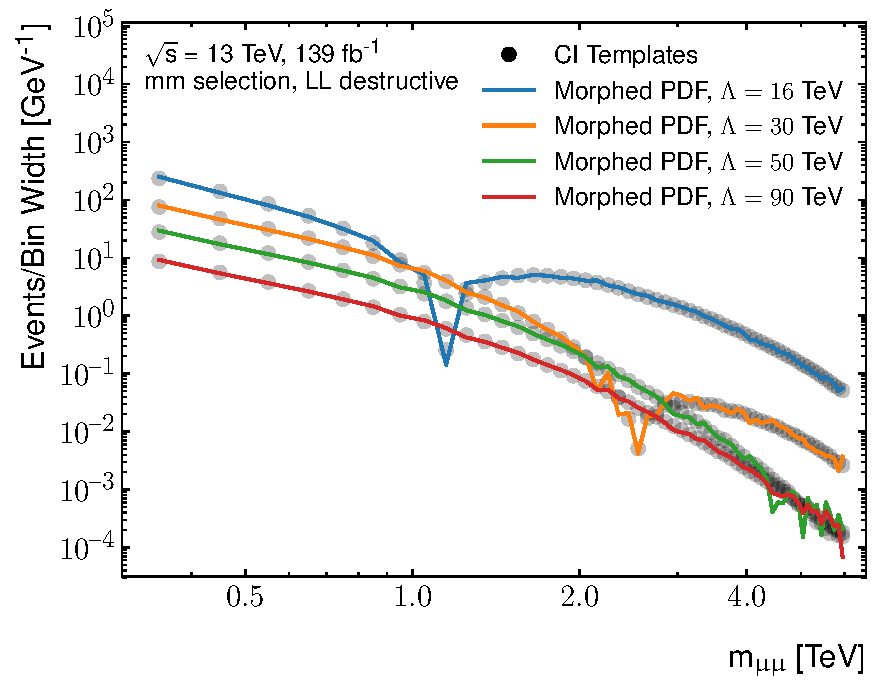
\includegraphics[width=\textwidth]{/Users/Deshan/Documents/PhD/thesis/Thesis/figures/analysis/bkgmodel/sigComp-dest-LL-mm.pdf}
        \label{fig:bkgmodel:Morphmm2}
    \end{subfigure}
    \caption[Morphed signal PDF produced at various $\Lambda$ values compared with the reweighted MC template.]{Comparison of morphed PDF signals for a CI signal for various $\Lambda$ values. for constructive (left) and destructive (right) interference for the electron (top) and muon (bottom) channels. Absolute number of events is plotted in each bin.}
    \label{fig:bkgmodel:Morph}
\end{figure}

\begin{figure}[h!]
    \centering
    \begin{subfigure}[b]{0.49\textwidth}
        \centering
        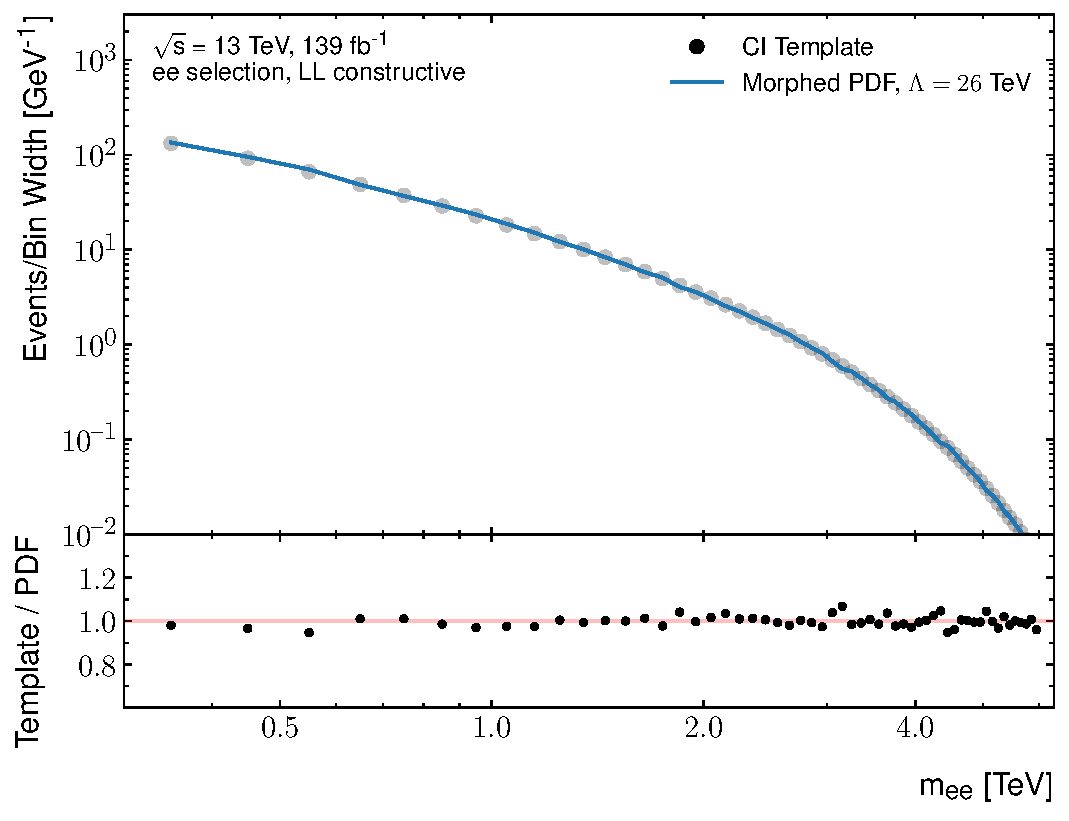
\includegraphics[width=\textwidth]{/Users/Deshan/Documents/PhD/thesis/Thesis/figures/analysis/bkgmodel/sigCompRatio-const-LL-ee.pdf}
        \label{fig:bkgmodel:ratioMorphee1}
    \end{subfigure}
    \begin{subfigure}[b]{0.49\textwidth}
        \centering
        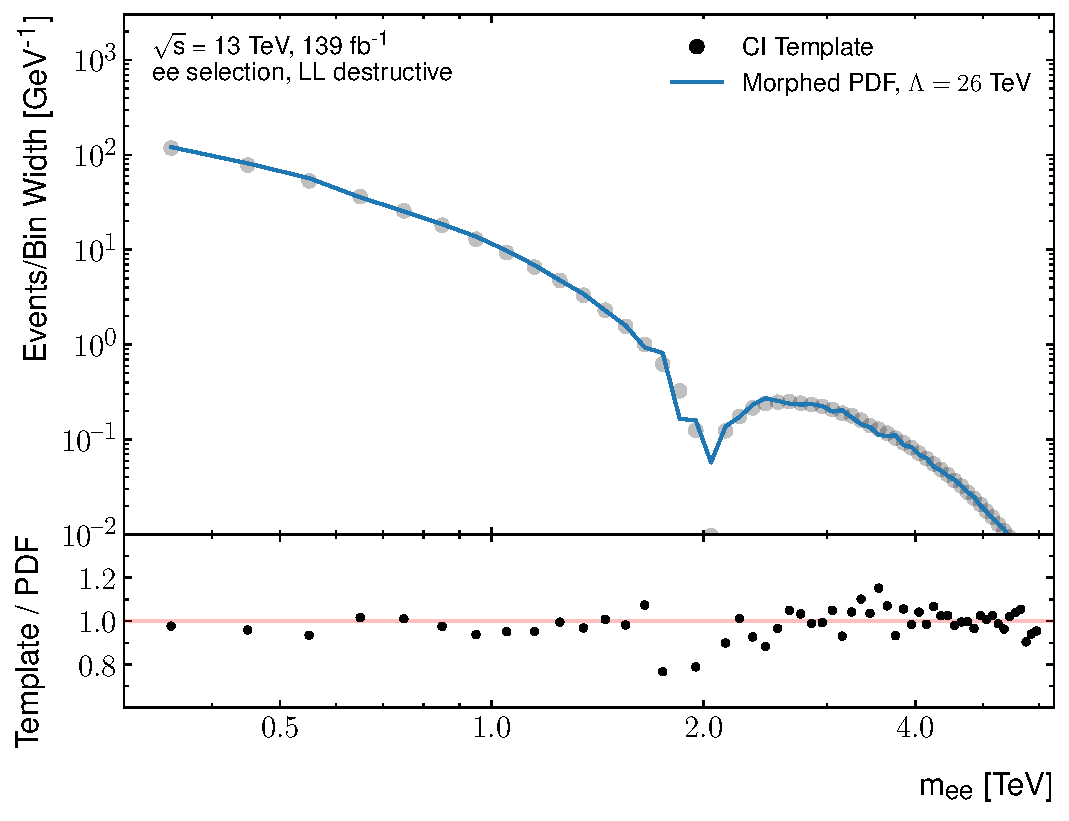
\includegraphics[width=\textwidth]{/Users/Deshan/Documents/PhD/thesis/Thesis/figures/analysis/bkgmodel/sigCompRatio-dest-LL-ee.pdf}
        \label{fig:bkgmodel:ratioMorphee2}
    \end{subfigure}
    \begin{subfigure}[b]{0.49\textwidth}
        \centering
        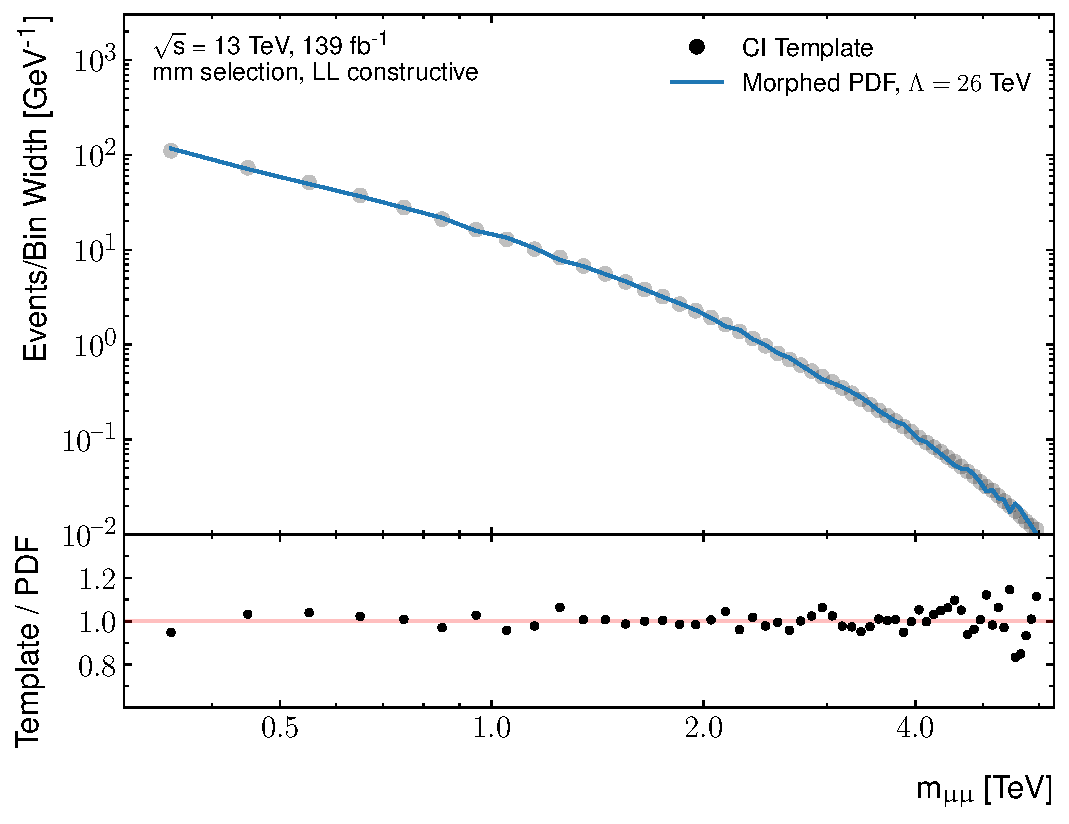
\includegraphics[width=\textwidth]{/Users/Deshan/Documents/PhD/thesis/Thesis/figures/analysis/bkgmodel/sigCompRatio-const-LL-mm.pdf}
        \label{fig:bkgmodel:ratioMorphmm1}
    \end{subfigure}
    \begin{subfigure}[b]{0.49\textwidth}
        \centering
        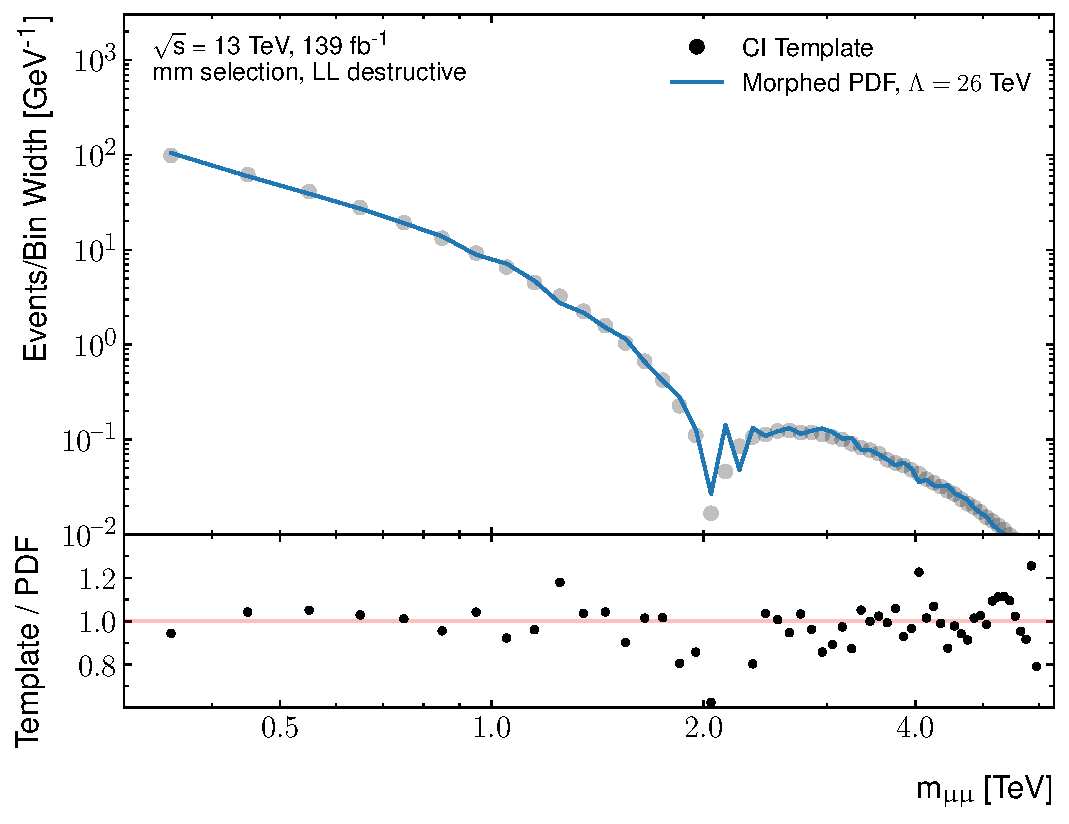
\includegraphics[width=\textwidth]{/Users/Deshan/Documents/PhD/thesis/Thesis/figures/analysis/bkgmodel/sigCompRatio-dest-LL-mm.pdf}
        \label{fig:bkgmodel:ratioMorphmm2}
    \end{subfigure}
    \caption[Comparison of morphed signal PDF with generated signal template]{Comparison of Morphed PDF signals for a CI signal with $\Lambda = \SI{26}{\tera\electronvolt}$ for constructive (left) and destructive (right) interference for the electron (top) and muon (bottom) channels. The bottom pad shows the ratio of the MC template with the morphed signal PDF. Absolute number of events is plotted in each bin.}
    \label{fig:bkgmodel:ratioMorph}
\end{figure}

\section{Estimation of fake background}\label{sec:datamc:fakes}
Processes involving jets or electron and a jet can be reconstructed as electrons in the algorithms, described in \cref{sec:reconstruction:electrons}, and pass the analysis selection. The dominant contribution for the electron plus jet final state is mainly due to the $W$+Jets processes. Light-flavour jets containing charged and neutral pions can be misidentified as electrons during reconstruction. Due to the high energies of collisions at the LHC, the decays of neutral pions, $\pi^0 \rightarrow \gamma\gamma$, are highly boosted and can lead to narrow electromagnetic energy depositions. These processes can give rise to signatures that are difficult to distinguish from those of the desired electrons. The desired electrons are referred to as \emph{real electrons}, whereas the objects which mimic the electrons are referred to as \emph{fake electrons}. The fake background is difficult to estimate using simulation. Therefore, data-driven techniques are often used. This is mainly due to increased computing power needed to model the detector simulation of many jet interactions with the detector. 

\subsection{Matrix method}
The analysis uses the likelihood matrix method~\cite{Varnes:2016nrb} to estimate the fake background contribution using two levels of electron identification criteria: a \emph{tight} (T) selection which corresponds to the nominal analysis selection, and a \emph{loose} (L) identification criteria which relaxes the nominal identification. The set of objects passing the \emph{tight} selection, $N_{tight}$, is a subset of those passing the \emph{loose} selection, $N_{loose}$. Pairs of electron candidates are considered denoted by $N_{xy}$ with $x,y \in T,L$, giving the number of electron pairs passing a specific selection. The fist index representing the leading electron ($p_{T,lead} > p_{T,sublead}$) and the second one the subleading electron. An additional set of quantities $N_{xy}$ with $x,y \in R,F$ can be defined to denote whether an electron is real (R) or fake (F). The relationship between the two sets of quantities is given by~\cite{EXOT-2016-05}

\begin{equation}\label{eq:matrix_method_1}
\left(\begin{array}{c}N_{TT}\\ N_{TL}\\ N_{LT}\\ N_{LL}\end{array}\right) = M \left(\begin{array}{c}N_{RR}\\ N_{RF}\\ N_{FR}\\ N_{FF}\end{array}\right) , M =
    \begin{pmatrix}
    r_1r_2 & r_1f_2 &  f_1r_2 & f_1f_2\\
    r_1\tilde{r2} & r_1\tilde{f2} & f_1\tilde{r2} & f_1\tilde{f2}\\
    \tilde{r1}r_2 & \tilde{r1}f_2 & \tilde{f1}r_2 & \tilde{f1}f_2\\
    \tilde{r1}\tilde{r2} & \tilde{r1}\tilde{f2} & \tilde{f1}\tilde{r2} & \tilde{f1}\tilde{f2}  
    \end{pmatrix}
\end{equation}

where $\tilde{x} = 1 - x$. The vectors on the right- (left-) hand side contain exclusive measurable (not measurable) quantities, e.g. L would denote an electron that passes the \emph{loose} selection and not the \emph{tight} selection. The coefficients $r$ and $f$ correspond to the real and fake rates, respectively. The real efficiency is the probability of real electrons to be reconstructed as \emph{tight} electrons and is calculated using MC. In contrast, the fake efficiency is the probability of a fake electron selected as \emph{loose} to be reconstructed as a \emph{tight} electron. The fake efficiency is calculated using data. Index 1 and 2 correspond to the efficiencies of the leading and subleading electrons. 

The number of misidentified events within the electron selection is estimated by measuring the number of events passing the signal selection ($N_{TT}$), which contains at least one fake electron. These fake events arise from events where at least one electron is misidentified (RF and FR), or events where both electrons are misidentified (RR). The total number of fake electrons is be then obtained from the sum of these contributions

\begin{equation}
    \begin{aligned}\label{eq:mm:nfakes}
    & N^{\text{fake}}_{TT}=r_1f_2N_{RF}+f_1r_2N_{FR}+f_1f_2N_{FF} ,
    \end{aligned}
\end{equation}

A likelihood is formed to include poisson constraints on $N_{xy}$ with $x,y \in T,L$:
\begin{equation}
    \mathcal{L} = \prod_{x,y \in T,L} P(N_{xy},N_{xy}^{pred}), 
\end{equation}
where \emph{P} represents the Poisson constraint on the observed number of events in each electron category and is consistent with the predicted number of fake and real leptons. The predicted values can be expressed in terms of a linear combination of $N_{xy}$ with $x,y \in R,F$ terms by using \cref{eq:matrix_method_1}
\begin{equation}
    \begin{aligned}
    N_{TL}^{pred} = (r_1r_2)N_{RR} + (r_1f_2)N_{RF} + (f_1r_2)N_{FR} + (f_1f_2)N_{RR},  \\
    N_{LT}^{pred} = (r_1\tilde{r_2})N_{RR} + (r_1\tilde{f_2})N_{RF} + (f_1\tilde{r_2})N_{FR} + (f_1\tilde{f_2})N_{RR}, \\
    N_{LL}^{pred} = (\tilde{r_1}\tilde{r_2})N_{RR} + (\tilde{r_1}\tilde{f_2})N_{RF} + (\tilde{f_1}\tilde{r_2})N_{FR} + (\tilde{f_1}\tilde{f_2})N_{RR}.
    \end{aligned}
\end{equation}

The likelihood is minimised, and the number of fakes can be extracted using \cref{eq:mm:nfakes}, which is then applied as an event by event weight used to produce an invariant mass distribution for the fake background contribution. The background template produced is smoothed using a functional fit~\cite{EXOT-2016-05}. 

The uncertainty on the functional fit is calculated by varying the start of the fit, which results in an envelop of possible estimates for the fitted template template. The start range of the fit is varied from \SI{130}{\giga\electronvolt} to \SI{150}{\giga\electronvolt} in steps of \SI{2}{\giga\electronvolt}. The resulting envelop of the fits are taken as the uncertainty of the fake electron estimate. The uncertainty of the fake estimation varies from from 50\% at \SI{2}{\tera\electronvolt} to 110\% at \SI{5}{\tera\electronvolt}. 

\section{Transfer functions}\label{sec:datamc:transfer}
The Transfer function approach offers an alternative method to produce large statistic and smooth DY and \ttbar samples~\cite{Aad:2019fac,Falke:2693468}. This method is used to overcome the limitations of insufficient MC statistics at lower invariant masses. The available MC samples for the previous analysis using the $2015-16$ dataset~\cite{EXOT-2016-05} had statistical uncertainties that the same as the statistical uncertainty in data, resulting in a loss of sensitivity to new physics models. Consequently, complicated background smoothing techniques with functional fits were adopted in the analysis in an attempt to tackle the loss of sensitivity.

The TF approach provides a smooth transformation between the truth and reconstruction level invariant-mass spectrum. A functional form is not imposed on the TF, and the transformation is analytically parametrised using the detector resolution. The electron and muon channels require separate TFs due to the different reconstruction properties of the two channels.

\subsection{Overview}
The transition between a known truth spectrum, $S_t(m_{\ell\ell,t})$, and an unknown reconstructed spectrum, $S_r(m_{\ell\ell,r})$, is be parametrised by a TF, $P(m_{\ell\ell,r} \mid m_{\ell\ell,t})$. The TF describes the probability to reconstruct an event at invariant mass of $m_{\ell\ell,r}$ for events with truth mass $m_{\ell\ell,t}$ that passes the selection. Full simulation MC is used to construct the TFs. The TFs are obtained fitting the detector response, with simultaneous fits to $m_{\ell\ell,t}$ bins, where the convolution of a Gaussian and a Crystal-ball is used to model the detector response. The truth invariant mass spectrum is obtained from very large truth-only MC samples. Larger samples can be produced at truth-level efficiently compared to fully reconstructed samples due to significantly smaller CPU times and disk space required to produce them. The truth-only sample is produced such that it is produced at luminosity 55 times larger than the available dataset. The following convolution is used to obtain the reconstruction level spectrum: 
\begin{equation}\label{eq:TF_generalConv}
	S_r(m_{\ell\ell,r}) = P(m_{\ell\ell,r} \mid m_{\ell\ell,t}) \otimes \left[ S_t(m_{\ell\ell,t}) \cdot A\varepsilon(m_{\ell\ell,t}) \right], 
\end{equation}
where $A\varepsilon(m_{\ell\ell,t})$ is the acceptance times efficiency. $A\varepsilon(m_{\ell\ell,t})$ is the probability that a event with truth invariant mass passes the selection. The probability is calculated by taking the fraction of events accepted in a truth invariant mass bin and the total number of generated events in that bin. 

% \subsection{Parametrisation of detector response}
% The TFs are obtained by fitting the detector response, $P(\mathcal{R} \mid m_{\ell\ell}^{truth})$, with a simultaneous fit on 200 $m_{\ell\ell}^{truth}$ bins. The detector response, $\mathcal{R}$, is used as the main variable in the fit due to it's mean value expected to be zero for each truth bin, and is defined as $\mathcal{R} = (m_{\ell\ell}^{reco} - m_{\ell\ell}^{truth}/ m_{\ell\ell}^{truth})$. To capture the response in the tail regions, a range of $R \in [-0.2,0.1]$ and $R \in [-0.75,0.75]$ is fitted for the electron and muon channels respectively. The range is chosen to cover the effects of the detector resolutions in the low and high invariant mass regions for both channels. 

% The convolution of a Gaussian and Crystal-ball function is used to model $P(\mathcal{R} \mid m_{\ell\ell}^{truth})$ after several functions were tested. The Gaussian, G, component of the function is chosen to model the main peak of the detector response, whereas the long tails of the Crystal-Ball, CB, models the tails of the detector response. The tails of the response in the electron channel are caused by electromagnetic radiation due to Bremsstrahlung. In the muon channel, the tails are a result of poorly reconstructed muons. The function is defined as: 
% \begin{equation}\label{eq:TF_responseParam}
%     P(\mathcal{R}) = \kappa \cdot \mathrm{CB}(\mathcal{R}| \mu_\mathrm{CB}, \sigma_\mathrm{CB}, \alpha_\mathrm{CB}, n_\mathrm{CB}) + (1 - \kappa) \cdot \mathrm{Gauss}(\mathcal{R}| \mu_\mathrm{G}, \sigma_\mathrm{G}).
% \end{equation}
% where,  $\mu_\mathrm{CB}$ and $\mu_\mathrm{G}$ are the mean values of the CB and G, respectively. $\mu_i$ is expected to be zero due to the definition of $\mathcal{R}$. $\sigma_\mathrm{CB}$ and $\sigma_\mathrm{G}$ are the width parameters of the CB and Gaussian components, respectively. $\alpha_\mathrm{CB}$ is the cut-off for the CB after which the Gaussian behaviour is replaced by a power-law. $n_\mathrm{CB}$ is the exponent of the power-law, and $\kappa$ is the fraction of the CB function in the total probability density function.

% The parameters of the response functions are then parameterised as a function of $m_{\ell\ell}^{truth}$ to allow for simultaneous fits in all $m_{\ell\ell}^{truth}$ regions. Initial values for the parameters are obtained by fitting the detector response in single $m_{\ell\ell}^{truth}$ regions. The simultaneous fits are performed, and the final detector response is obtained as:
% \begin{equation}\label{eq:TF_responseTransformation}
%     \begin{aligned}
%         & \mu_i(m_{\ell\ell}^{truth}) \to \mu_i'(m_{\ell\ell}^{truth}) = \left(\mu_i(m_{\ell\ell}^{truth}) \cdot m_{\ell\ell}^{truth}\right) + m_{\ell\ell}^{truth}, \\
%         & \sigma_i(m_{\ell\ell}^{truth}) \to \sigma_i'(m_{\ell\ell}^{truth}) = \sigma_i(m_{\ell\ell}^{truth}) \cdot m_{\ell\ell}^{truth},
%     \end{aligned}
% \end{equation}

\section{Data and background comparisons}\label{sec:datamc:compare}
\cref{fig:datamc:eecompare,fig:datamc:mmcompare} show the comparisons of the invariant mass distributions between the data and MC expectation with the addition of some benchmark CI interaction signals overlaid on top. The fake electron contribution was only estimated for the invariant-mass distributions \cref{fig:datamc:pt1,fig:datamc:pt2} show the \pt distributions for the leading and subleading leptons. 

The $\eta$ distributions for the leading and subleading leptons are shown in \cref{fig:datamc:eta1,fig:datamc:eta2}. In the electron channel, the maximum can be seen at $\eta = 0$ and falls towards higher values of $\abs{\eta}$. The transition region corresponds to $1.37 < \abs{\eta} < 1.52$. The muon channel shows dips in the $\eta$ distributions that correspond to poorly aligned chambers in the muon spectrometer. \cref{fig:datamc:phi1,fig:datamc:phi2} show the $\phi$ distributions for the leading and subleading leptons. A flat distribution is shown in the electron channel. The $\phi$ distribution for muons show small dips due to support structures on which the ATLAS detector is placed. 

The comparison is mainly produced for illustrative purposes, since the MC background prediction is used only for validation of the choice of functional fit. However, a good agreement is between the data and MC expectation is required for the MC to be used to validate the data-driven fit strategy. Furthermore, the comparisons allow for an early indication of issues that may have occurred when deciding on a selection.

\begin{figure}[]
    \centering
    \begin{subfigure}[b]{0.49\textwidth}
        \centering
        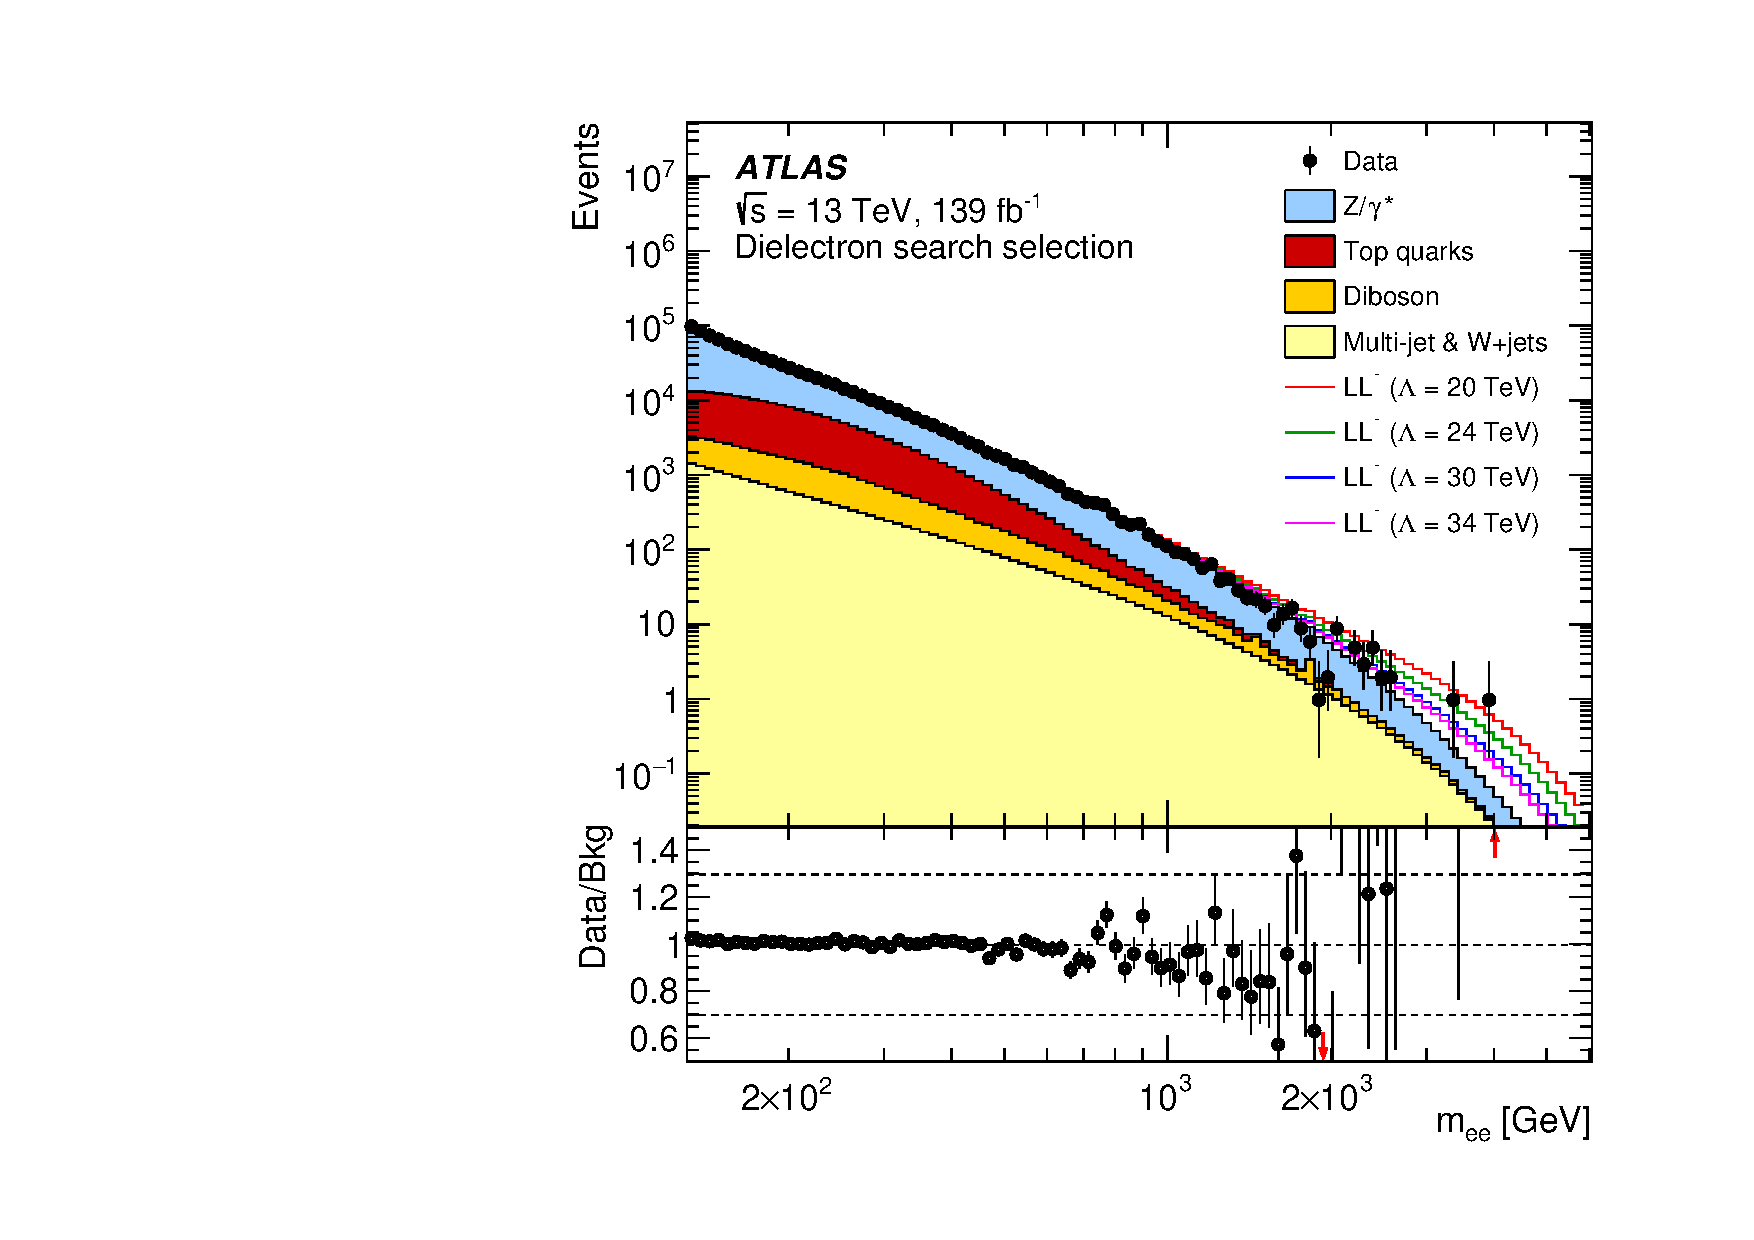
\includegraphics[width=\textwidth]{figures/analysis/datamc/dataMCcompare/figaux_01a.pdf}
        \label{fig:datamc:eeconst}
    \end{subfigure}
    \begin{subfigure}[b]{0.49\textwidth}
        \centering
        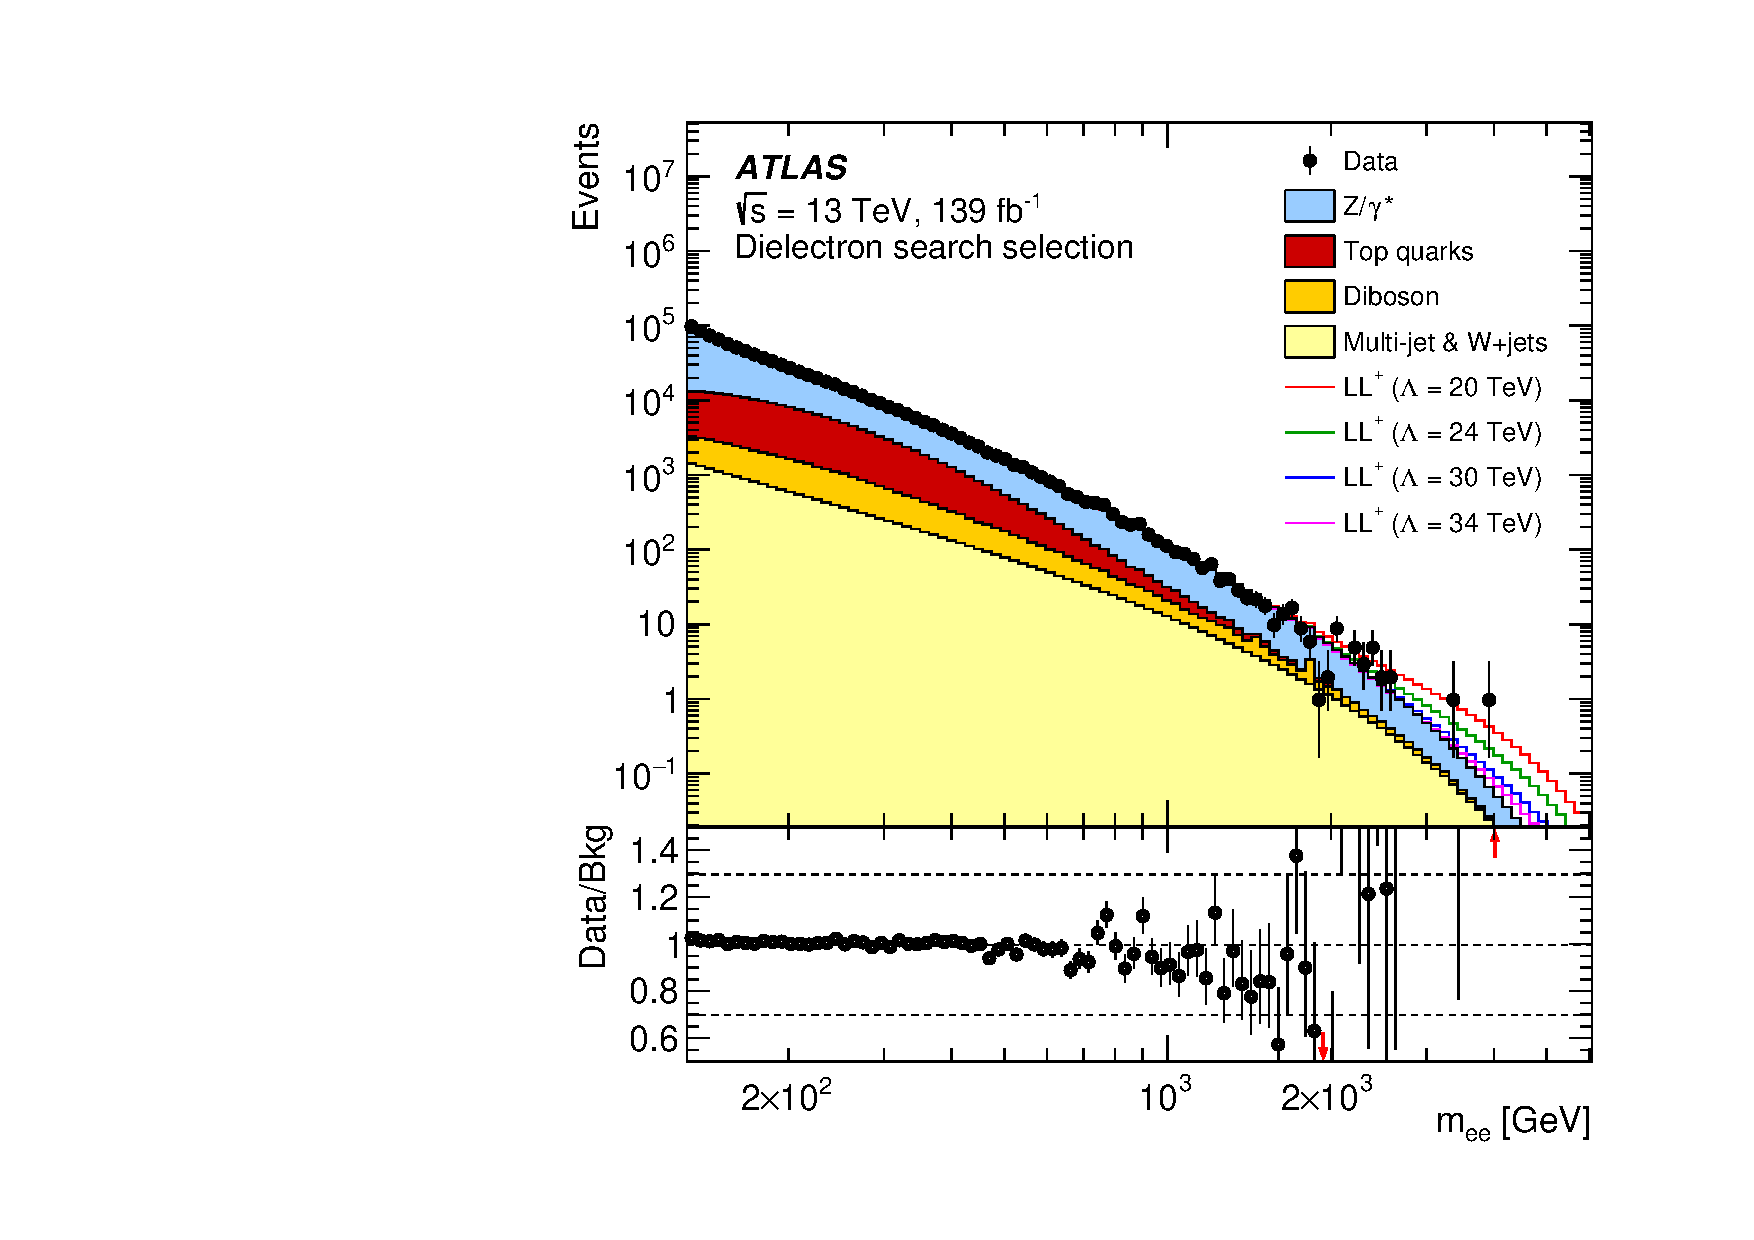
\includegraphics[width=\textwidth]{figures/analysis/datamc/dataMCcompare/figaux_01b.pdf}
        \label{fig:datamc:eedest}
    \end{subfigure}
    \caption[Invariant mass distributions for \ee channel]{Invariant mass distribution for the \ee selection for the full $2015-2018$ dataset and the respective MC campaign. The constructively interfering CI contributions are shown in (left),while destructive contributions are shown in (right). The bottom panel shows the ratio between the data and MC.}
    \label{fig:datamc:eecompare}
\end{figure}

\begin{figure}[]
    \centering
    \begin{subfigure}[b]{0.49\textwidth}
        \centering
        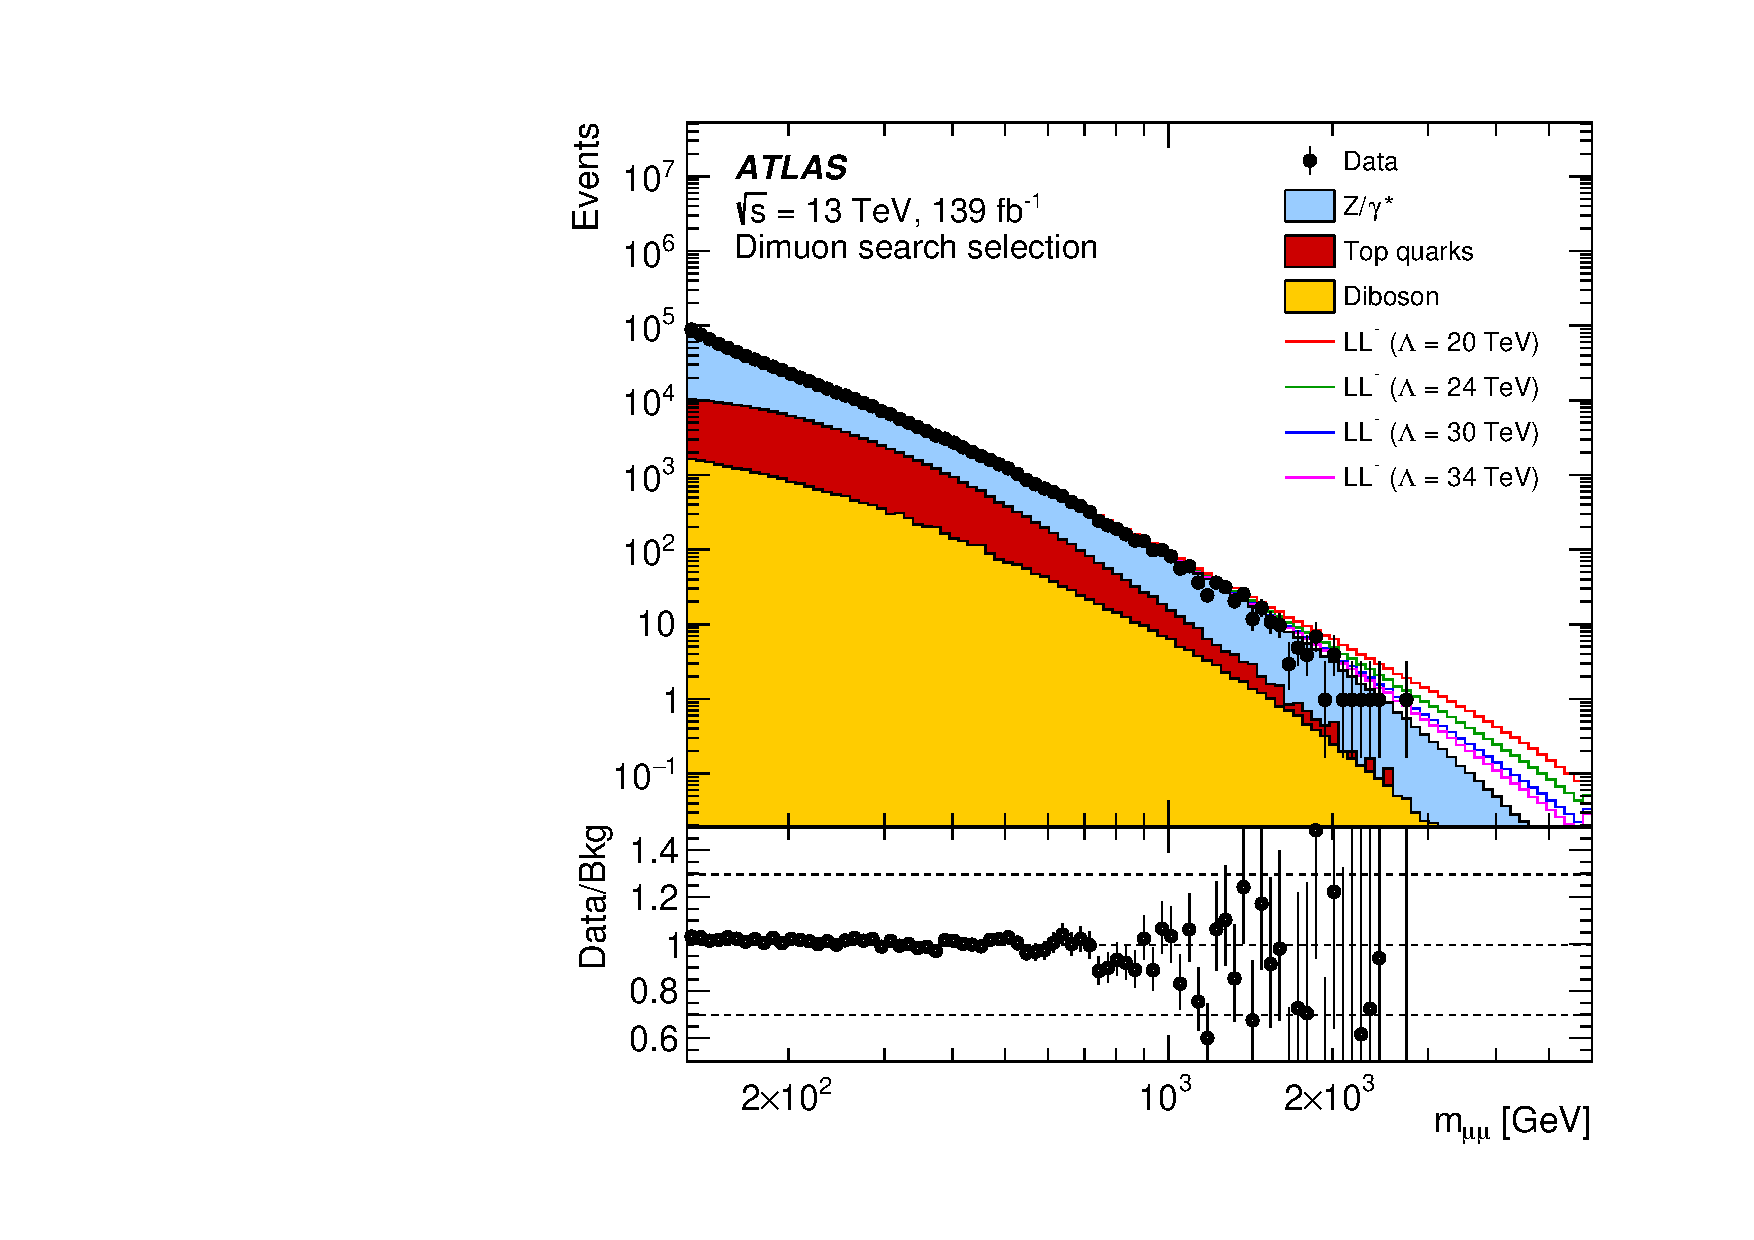
\includegraphics[width=\textwidth]{figures/analysis/datamc/dataMCcompare/figaux_02a.pdf}
        \label{fig:datamc:mmconst}
    \end{subfigure}
    \begin{subfigure}[b]{0.49\textwidth}
        \centering
        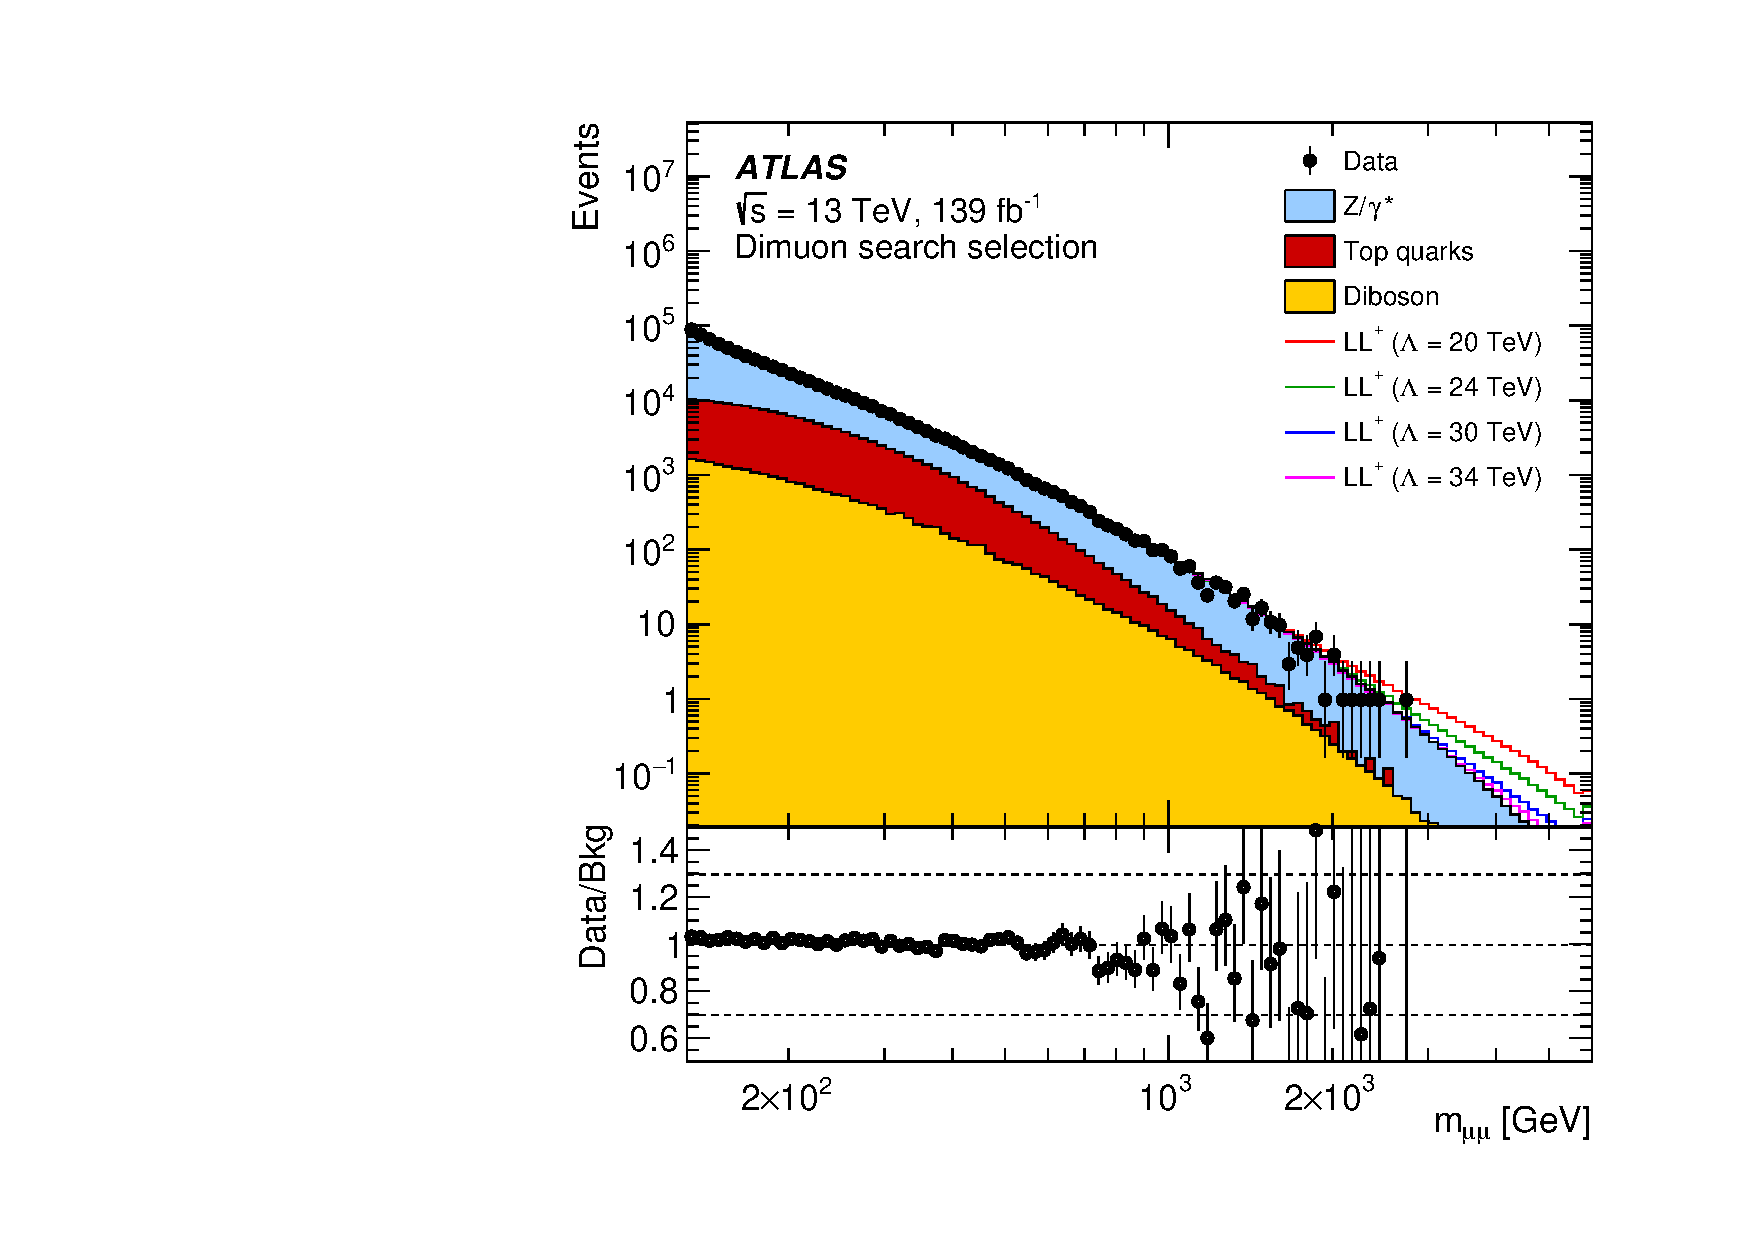
\includegraphics[width=\textwidth]{figures/analysis/datamc/dataMCcompare/figaux_02b.pdf}
        \label{fig:datamc:mmdest}
    \end{subfigure}
    \caption[Invariant mass distributions for \mumu channel]{Invariant mass distribution for the \mumu selection for the full $2015-2018$ dataset and the respective MC campaign. The constructively interfering CI contributions are shown in (left), while destructive contributions are shown in (right). The bottom panel shows the ratio between the data and MC.}
    \label{fig:datamc:mmcompare}
\end{figure}

\begin{figure}[]
    \centering
    \begin{subfigure}[b]{0.49\textwidth}
        \centering
        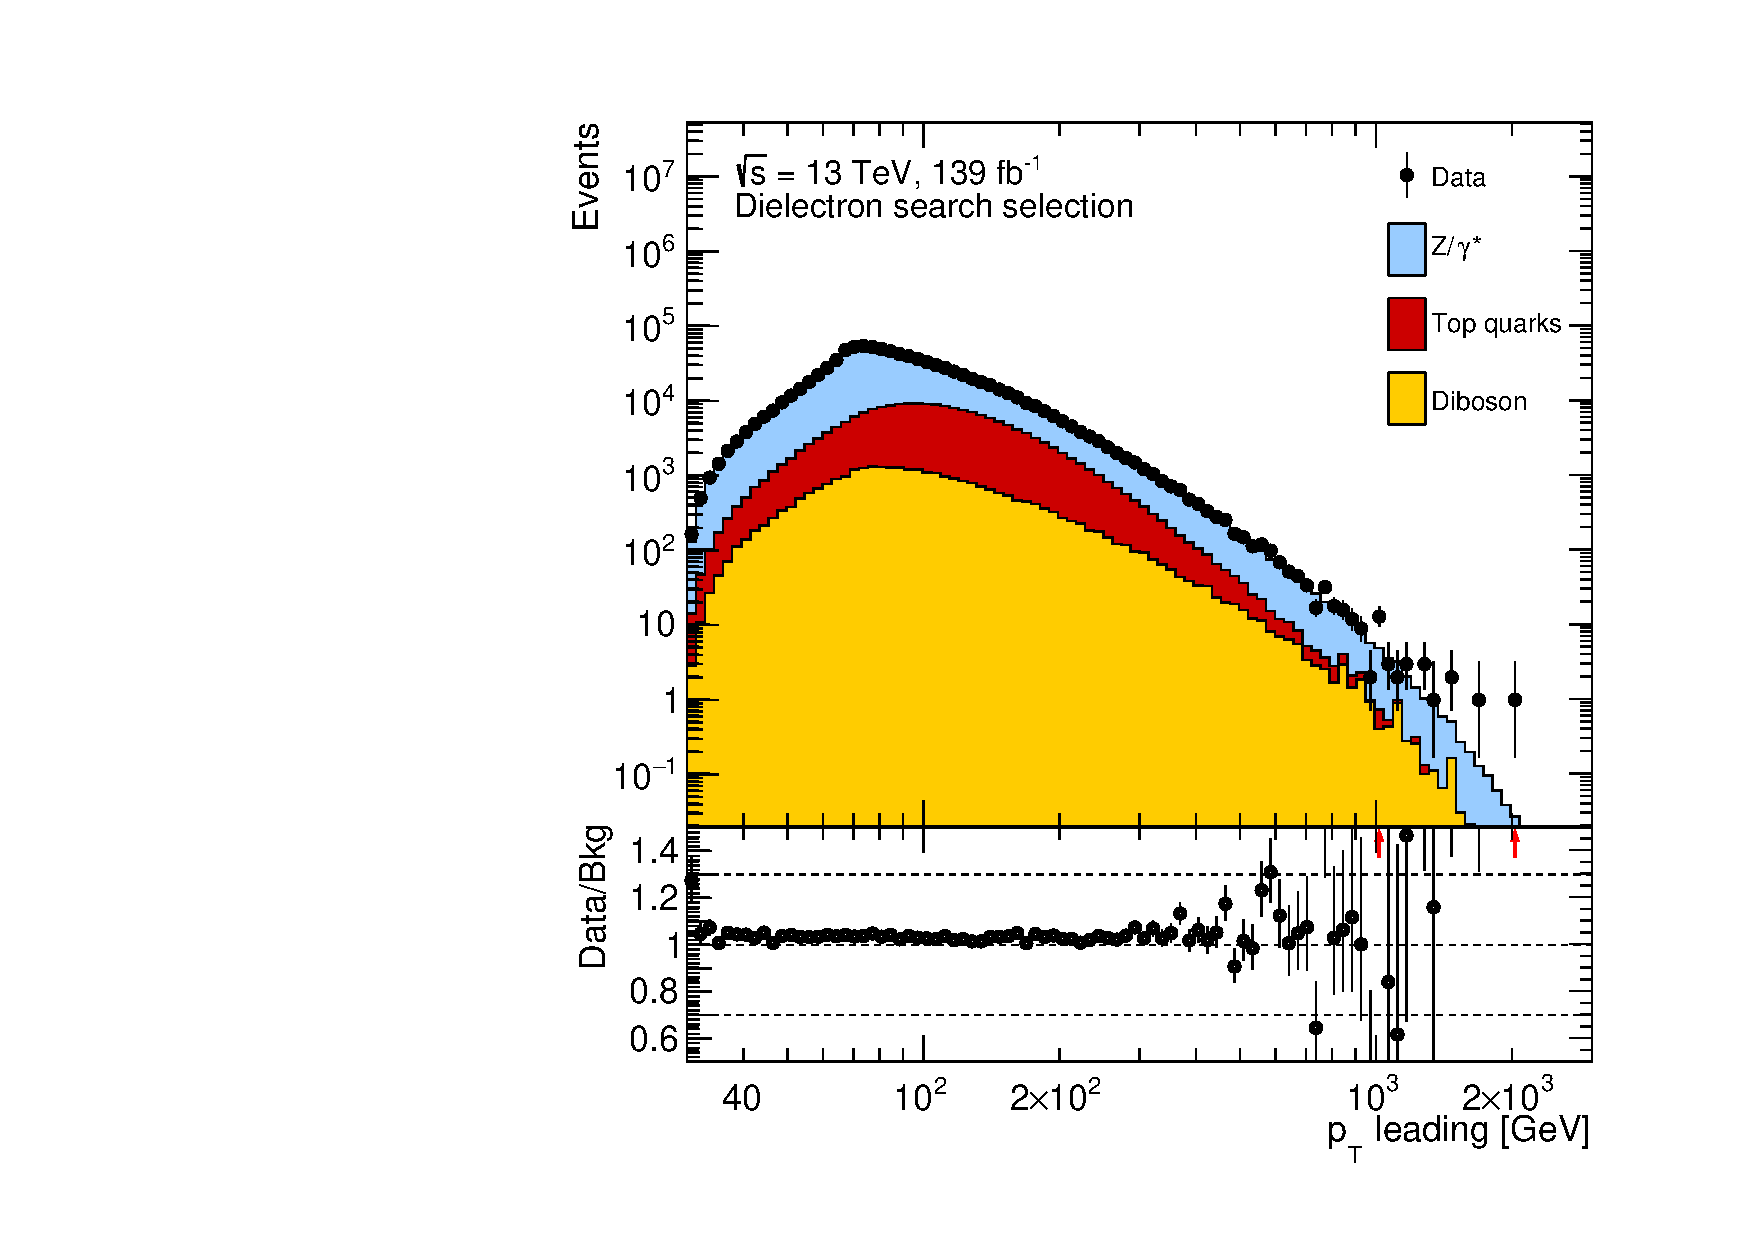
\includegraphics[width=\textwidth]{figures/analysis/datamc/dataMCcompare/ee_pt1_log100.pdf}
        \label{fig:datamc:eept1}
    \end{subfigure}
    \begin{subfigure}[b]{0.49\textwidth}
        \centering
        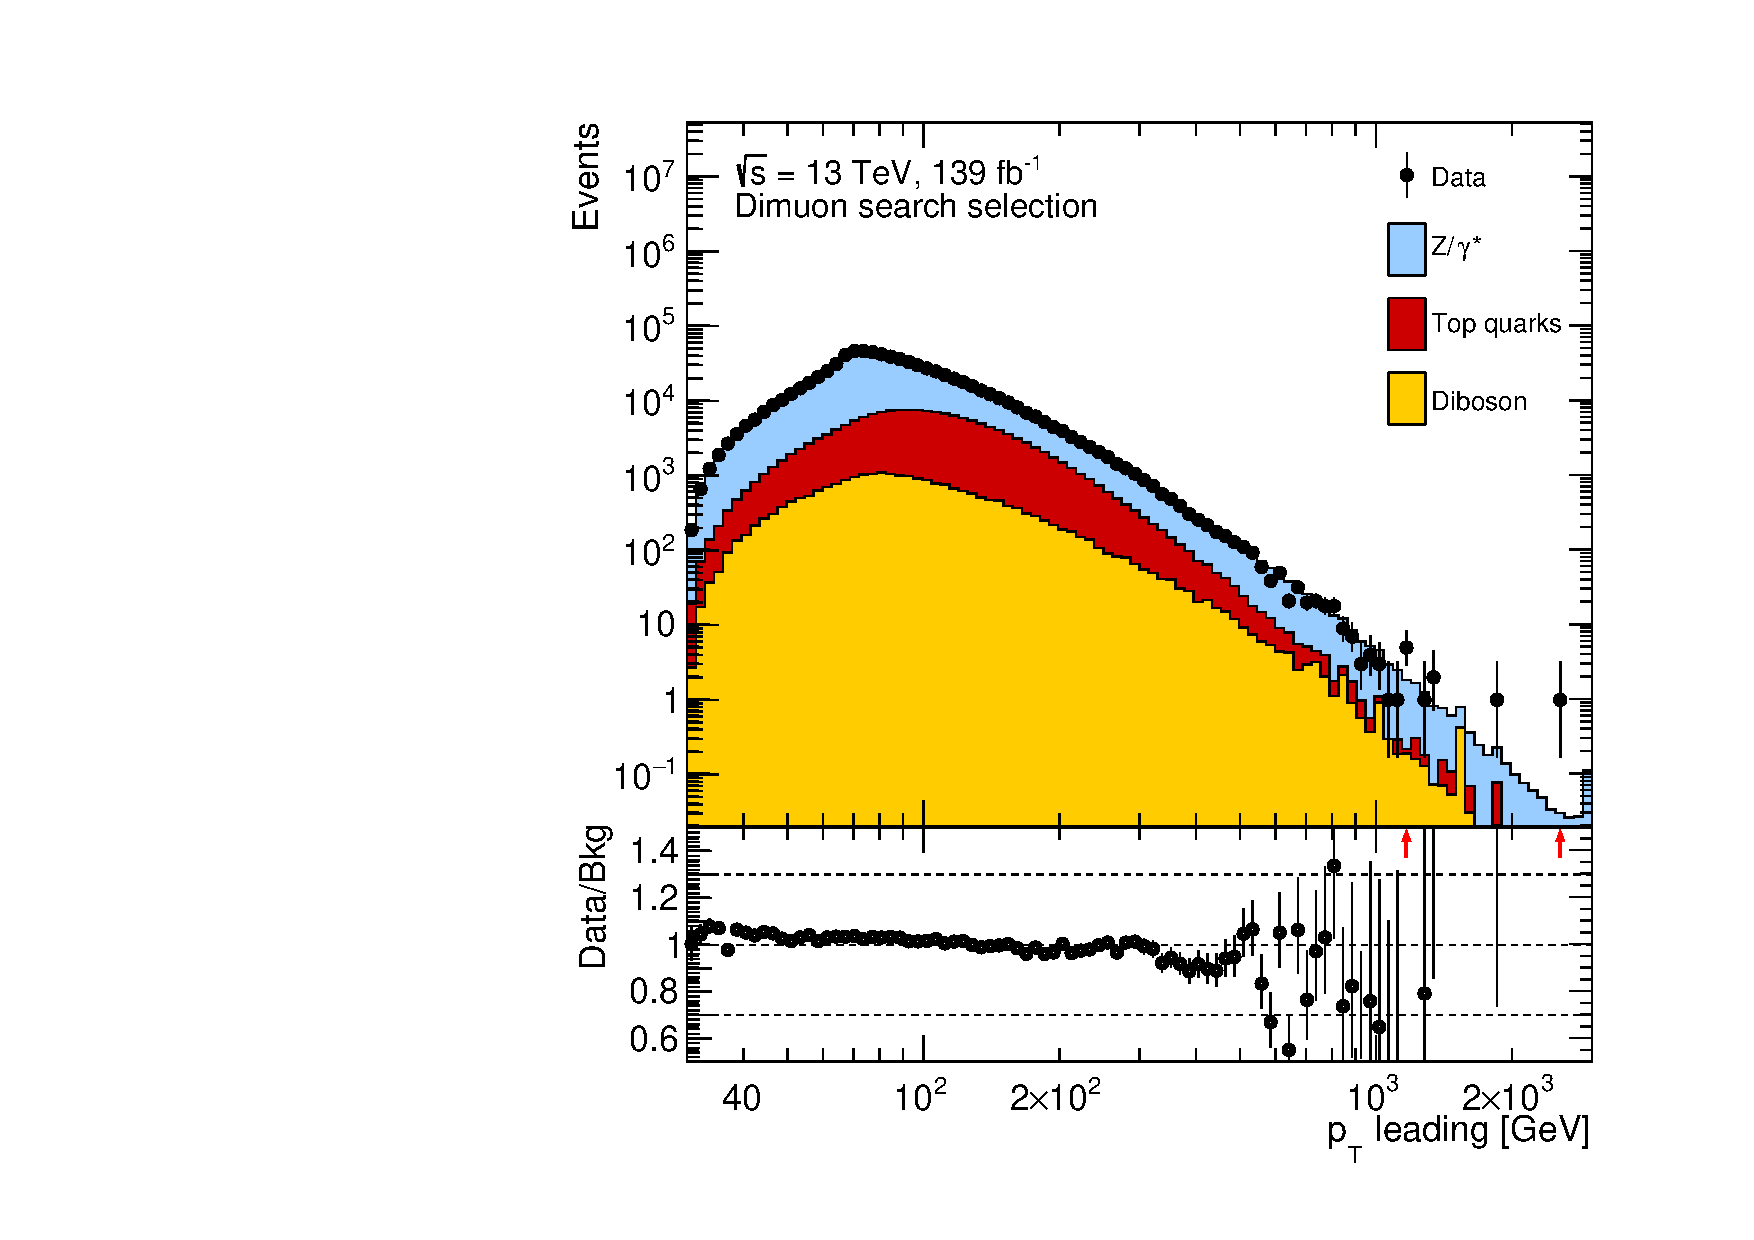
\includegraphics[width=\textwidth]{figures/analysis/datamc/dataMCcompare/uu_pt1_log100.pdf}
        \label{fig:datamc:uupt1}
    \end{subfigure}
    \caption[$p_\mathrm{T}$ distribution of the leading lepton for the dilepton selections for the full $2015-18$ dataset and the respective MC campaigns.]{$p_\mathrm{T}$ distribution of the leading lepton for the dilepton selections for the full $2015-18$ dataset and the respective MC campaigns. The \ee channel is shown in (left) and \mumu channel in (right). The bottom panel shows the ratio between the data and MC.}
    \label{fig:datamc:pt1}
\end{figure}

\begin{figure}[]
    \centering
    \begin{subfigure}[b]{0.49\textwidth}
        \centering
        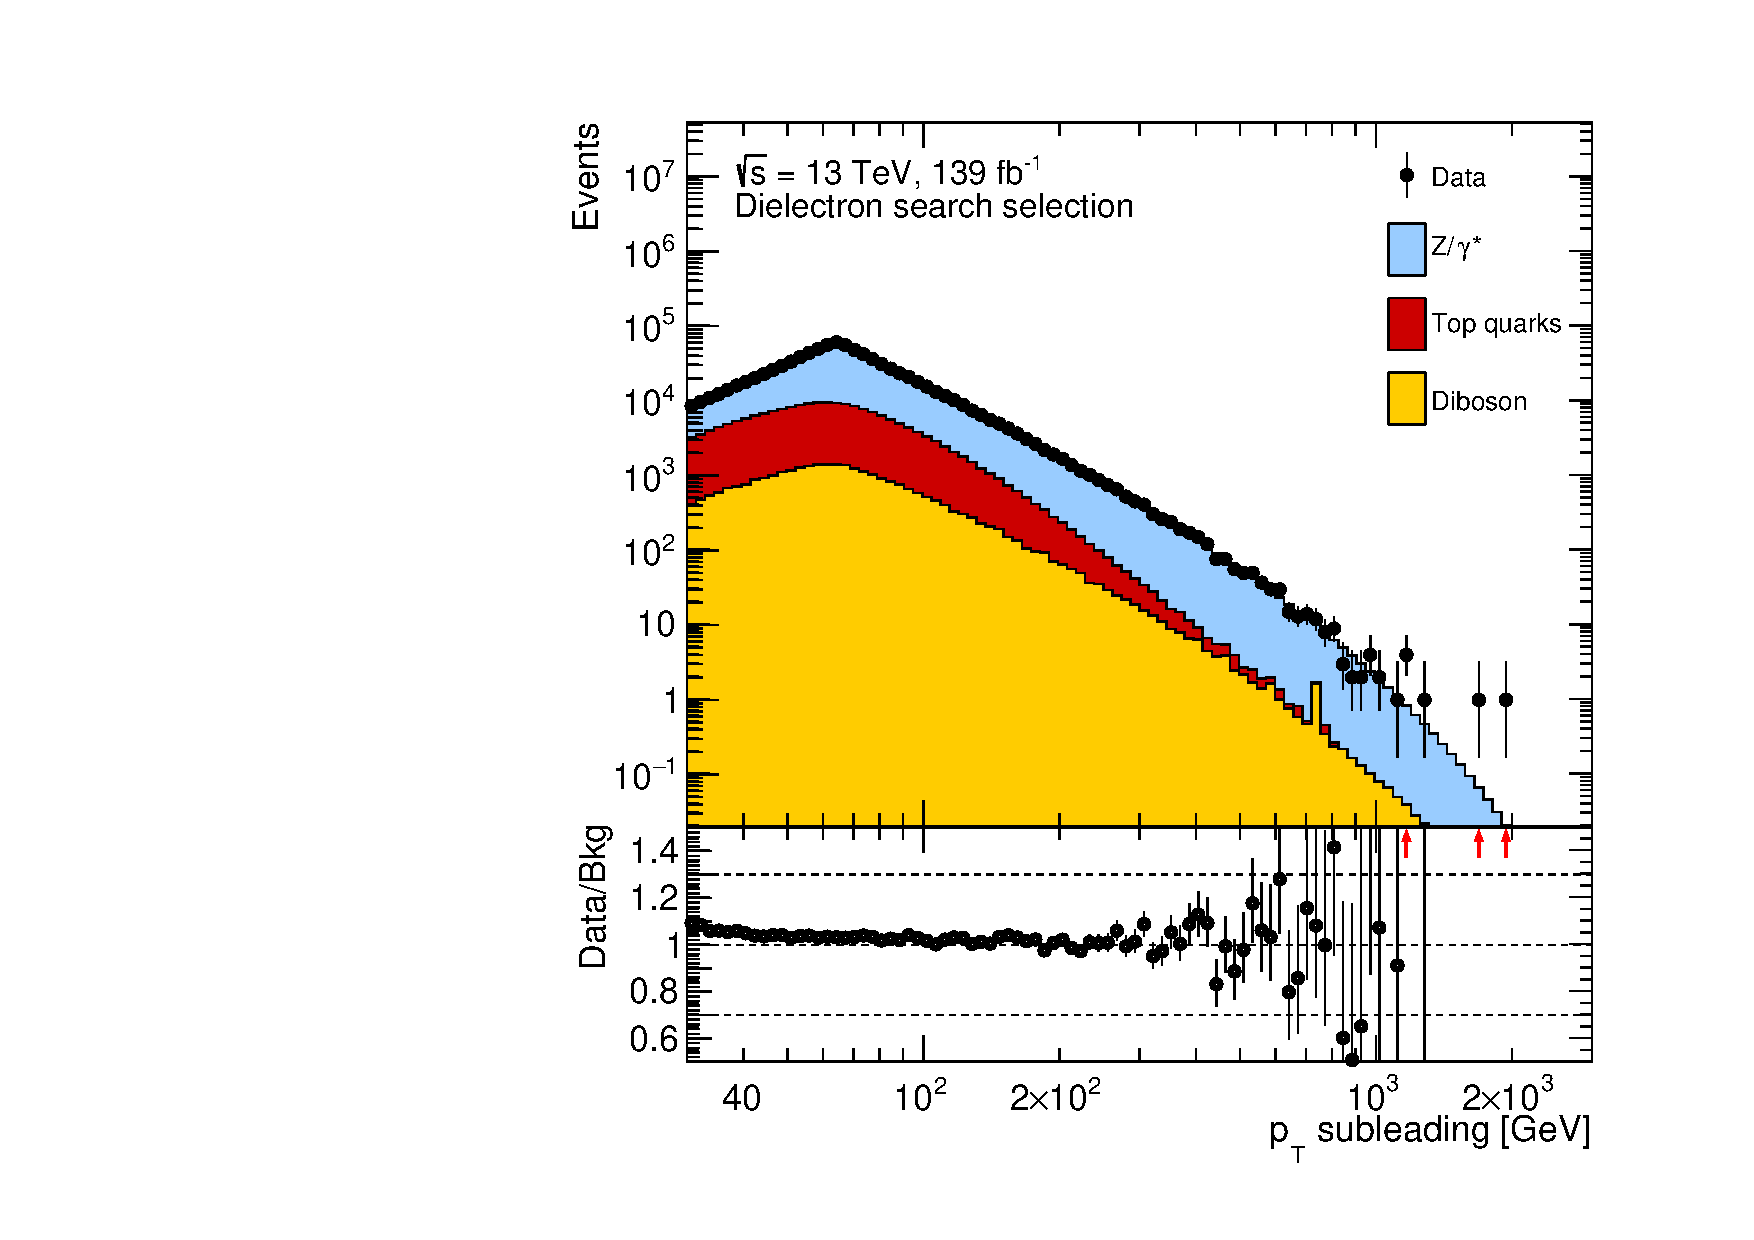
\includegraphics[width=\textwidth]{figures/analysis/datamc/dataMCcompare/ee_pt2_log100.pdf}
        \label{fig:datamc:eept2}
    \end{subfigure}
    \begin{subfigure}[b]{0.49\textwidth}
        \centering
        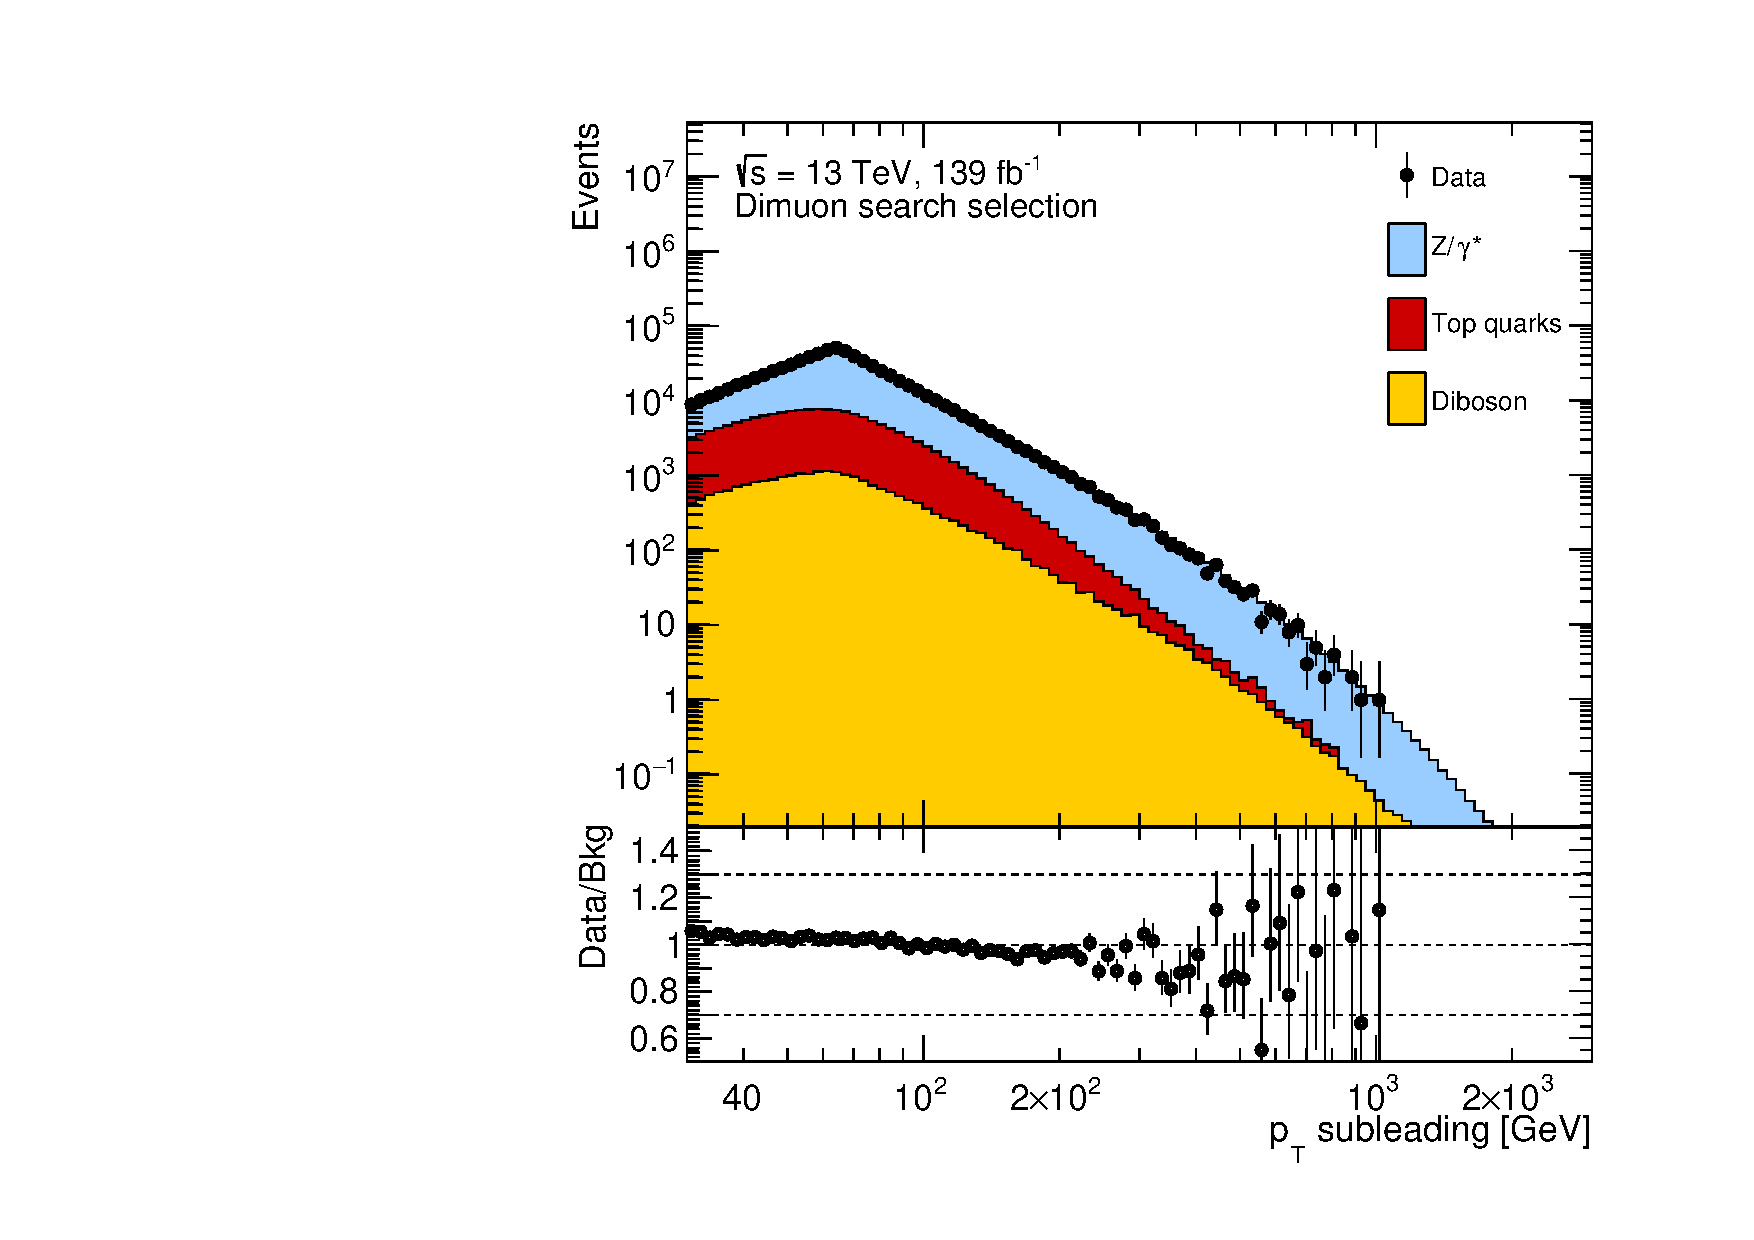
\includegraphics[width=\textwidth]{figures/analysis/datamc/dataMCcompare/uu_pt2_log100.pdf}
        \label{fig:datamc:uupt2}
    \end{subfigure}
    \caption[$p_\mathrm{T}$ distribution of the subleading lepton for the dilepton selections for the full $2015-18$ dataset and the respective MC campaigns.]{$p_\mathrm{T}$ distribution of the subleading lepton for the dilepton selections for the full $2015-18$ dataset and the respective MC campaigns. The \ee channel is shown in (left) and \mumu channel in (right). The bottom panel shows the ratio between the data and MC.}
    \label{fig:datamc:pt2}
\end{figure}

\begin{figure}[]
    \centering
    \begin{subfigure}[b]{0.49\textwidth}
        \centering
        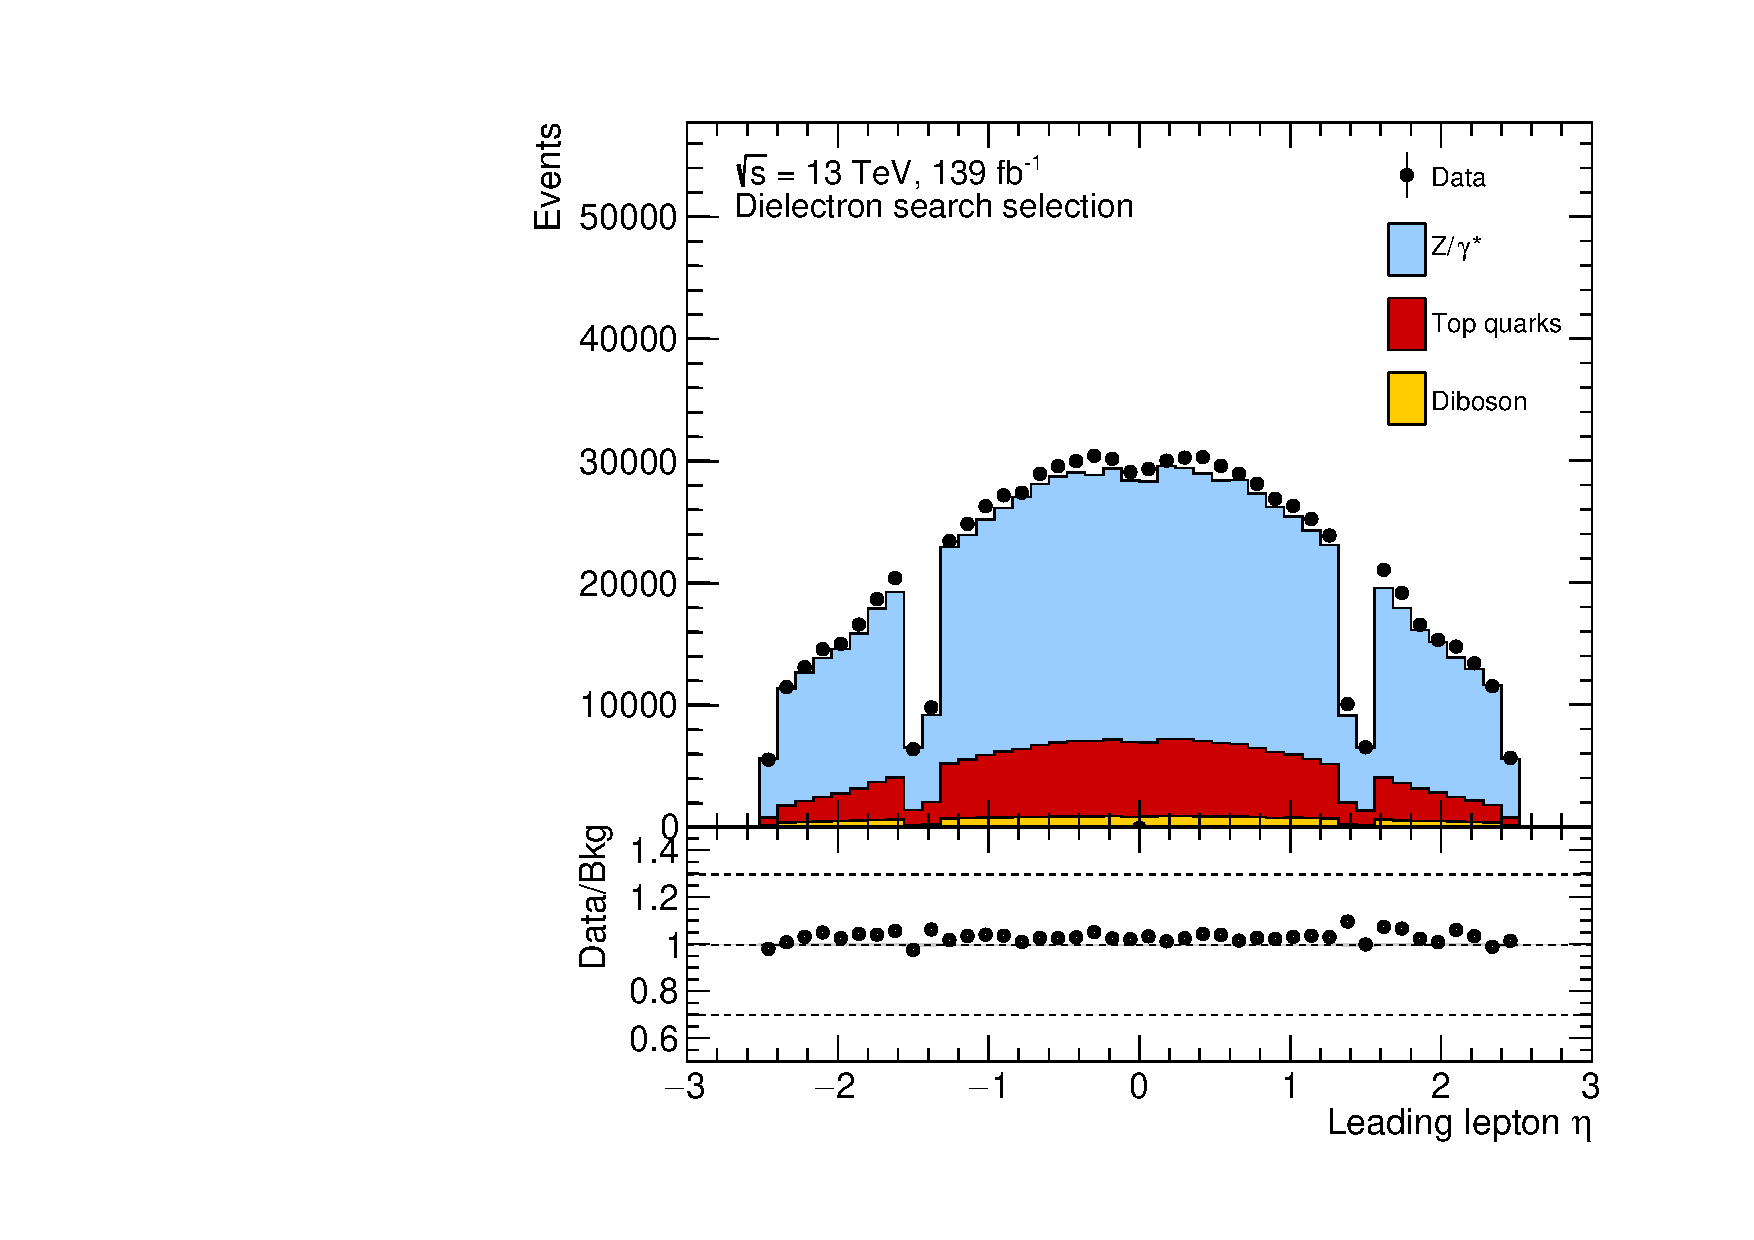
\includegraphics[width=\textwidth]{figures/analysis/datamc/dataMCcompare/ee_eta1.pdf}
        \label{fig:datamc:eeeta1}
    \end{subfigure}
    \begin{subfigure}[b]{0.49\textwidth}
        \centering
        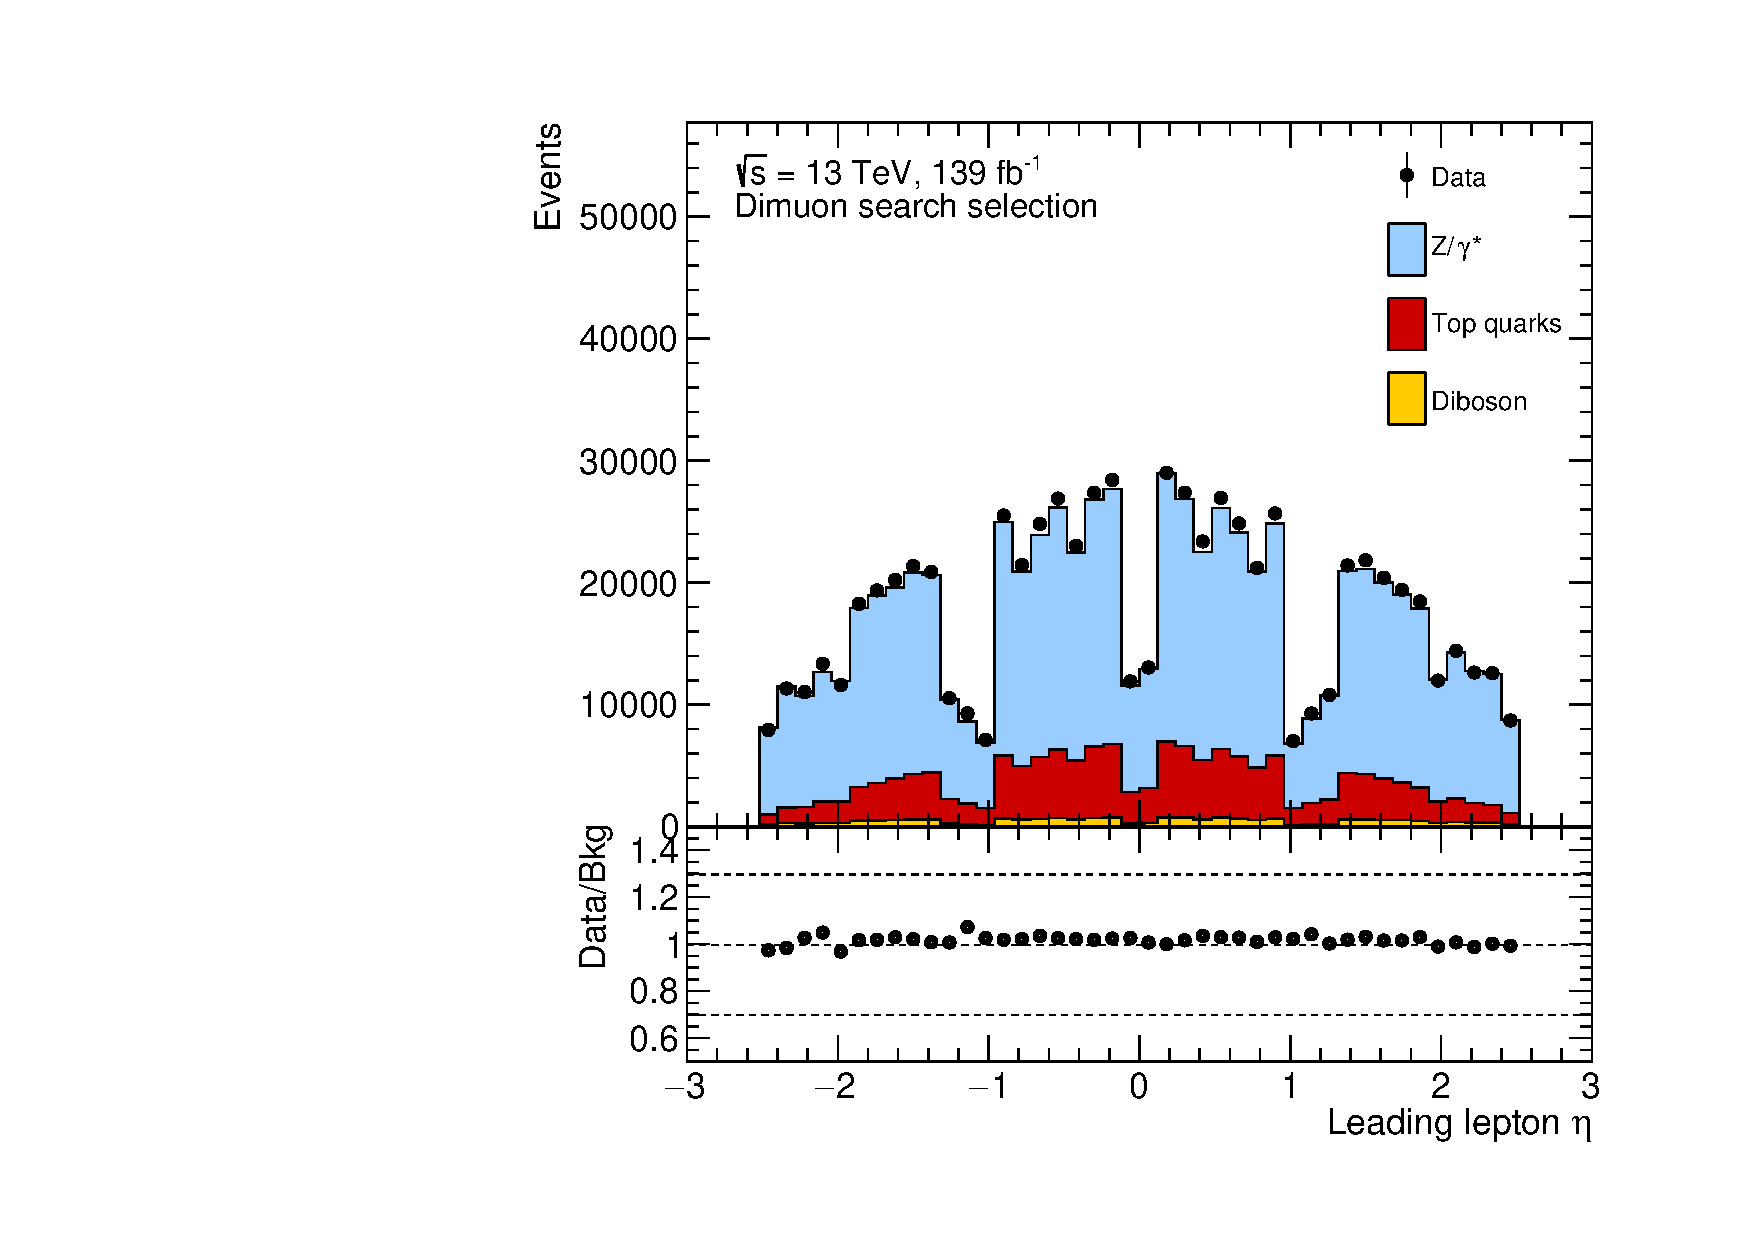
\includegraphics[width=\textwidth]{figures/analysis/datamc/dataMCcompare/uu_eta1.pdf}
        \label{fig:datamc:uueta1}
    \end{subfigure}
    \caption[$\eta$ distribution of the leading lepton for the dilepton selections for the full $2015-18$ dataset and the respective MC campaigns.]{$\eta$ distribution of the leading lepton for the dilepton selections for the full $2015-18$ dataset and the respective MC campaigns. The \ee channel is shown in (left) and \mumu channel in (right). The bottom panel shows the ratio between the data and MC.}
    \label{fig:datamc:eta1}
\end{figure}

\begin{figure}[]
    \centering
    \begin{subfigure}[b]{0.49\textwidth}
        \centering
        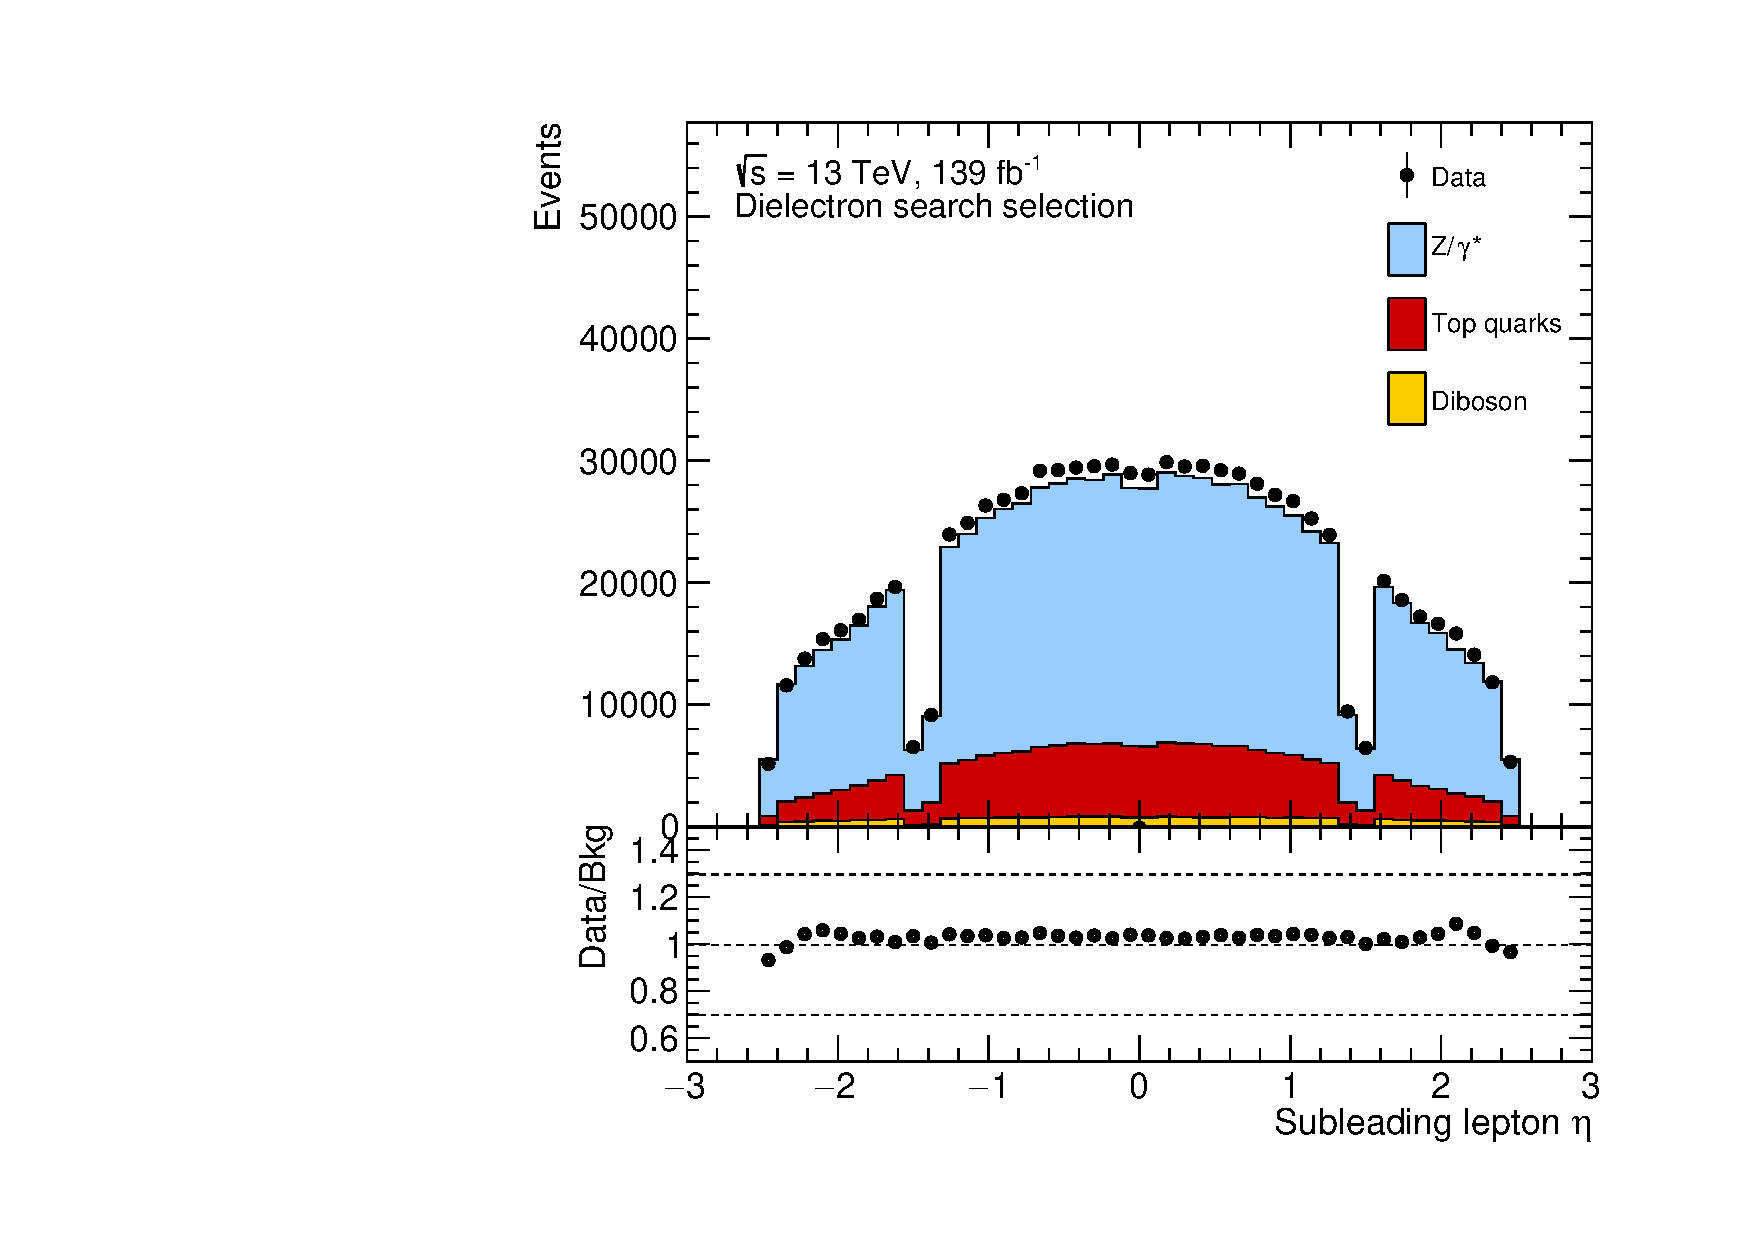
\includegraphics[width=\textwidth]{figures/analysis/datamc/dataMCcompare/ee_eta2.pdf}
        \label{fig:datamc:eeeta2}
    \end{subfigure}
    \begin{subfigure}[b]{0.49\textwidth}
        \centering
        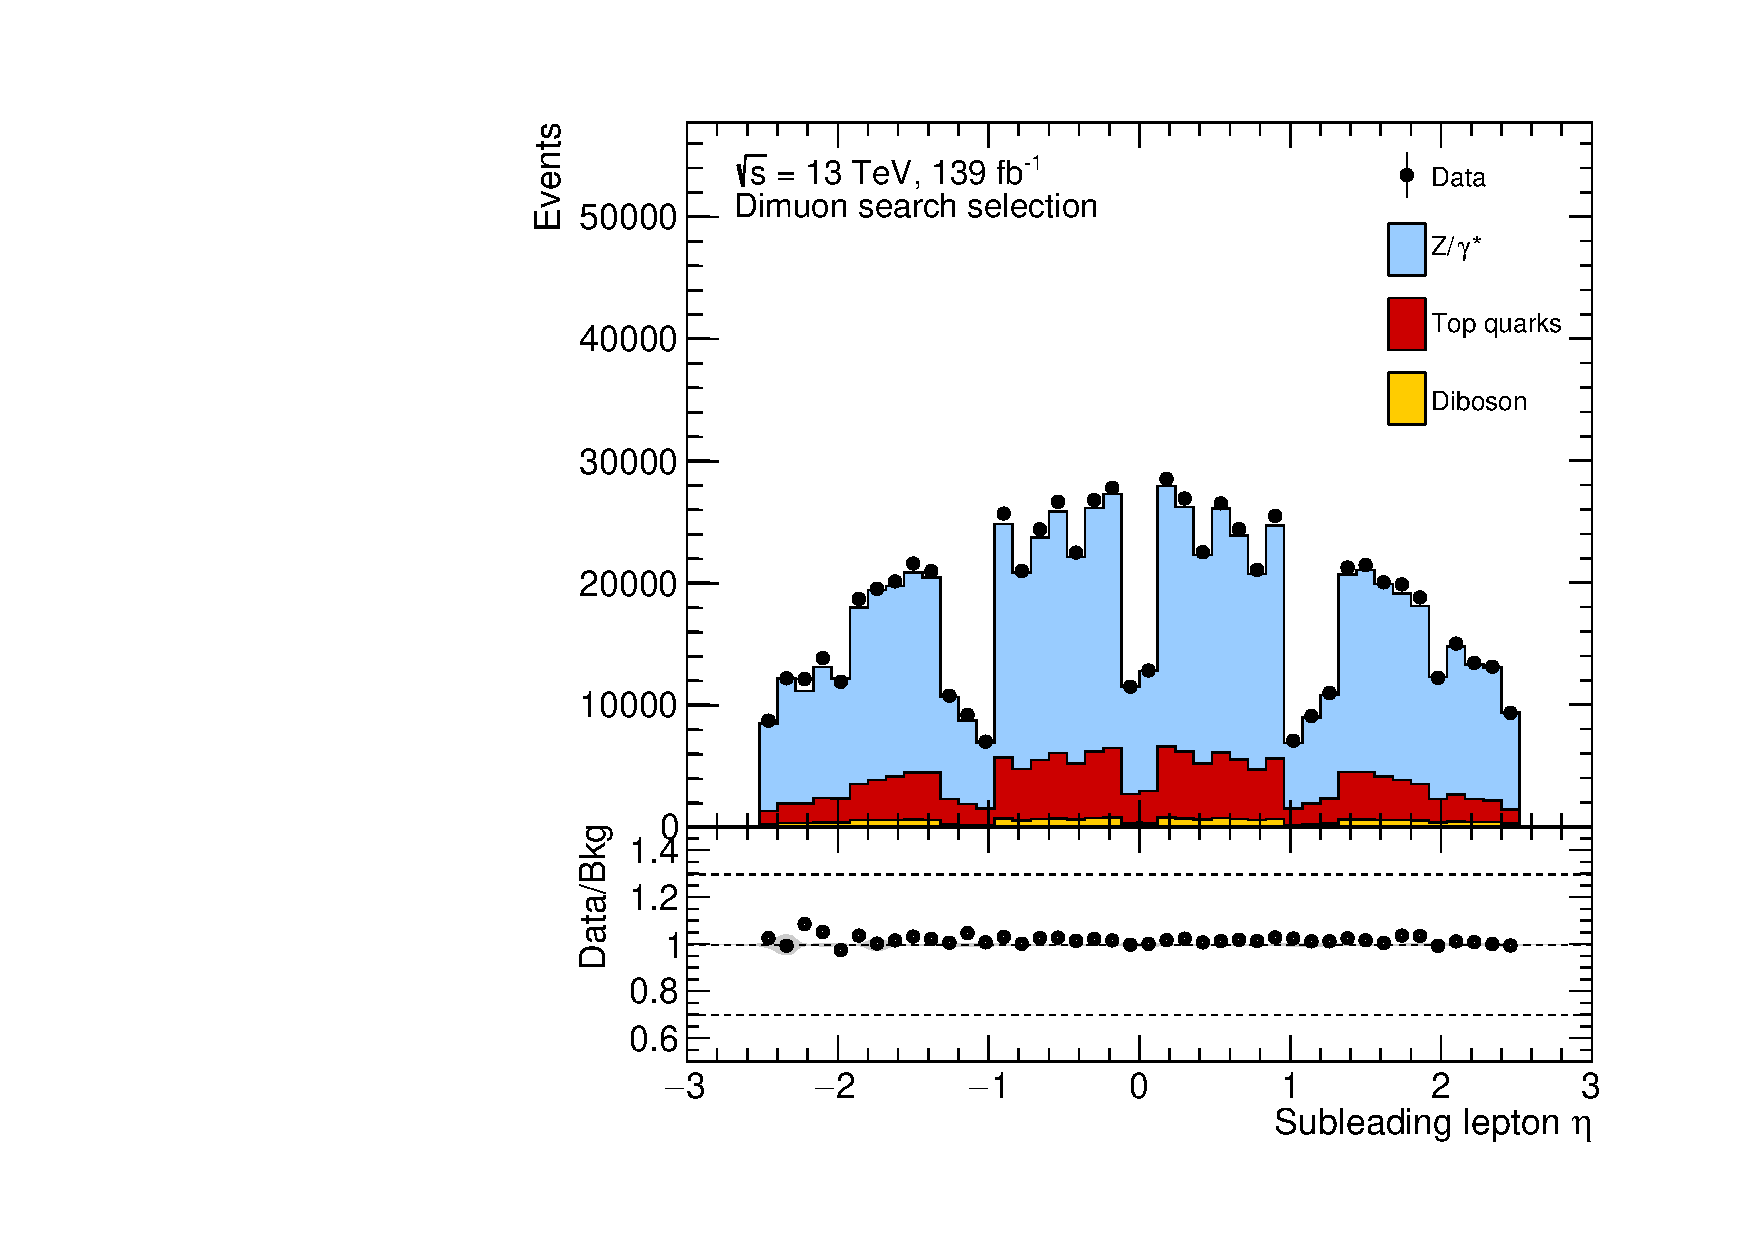
\includegraphics[width=\textwidth]{figures/analysis/datamc/dataMCcompare/uu_eta2.pdf}
        \label{fig:datamc:uueta2}
    \end{subfigure}
    \caption[$\eta$ distribution of the subleading lepton for the dilepton selections for the full $2015-18$ dataset and the respective MC campaigns.]{$\eta$ distribution of the subleading lepton for the dilepton selections for the full $2015-18$ dataset and the respective MC campaigns. The \ee channel is shown in (left) and \mumu channel in (right). The bottom panel shows the ratio between the data and MC.}
    \label{fig:datamc:eta2}
\end{figure}
\begin{figure}[]
    \centering
    \begin{subfigure}[b]{0.49\textwidth}
        \centering
        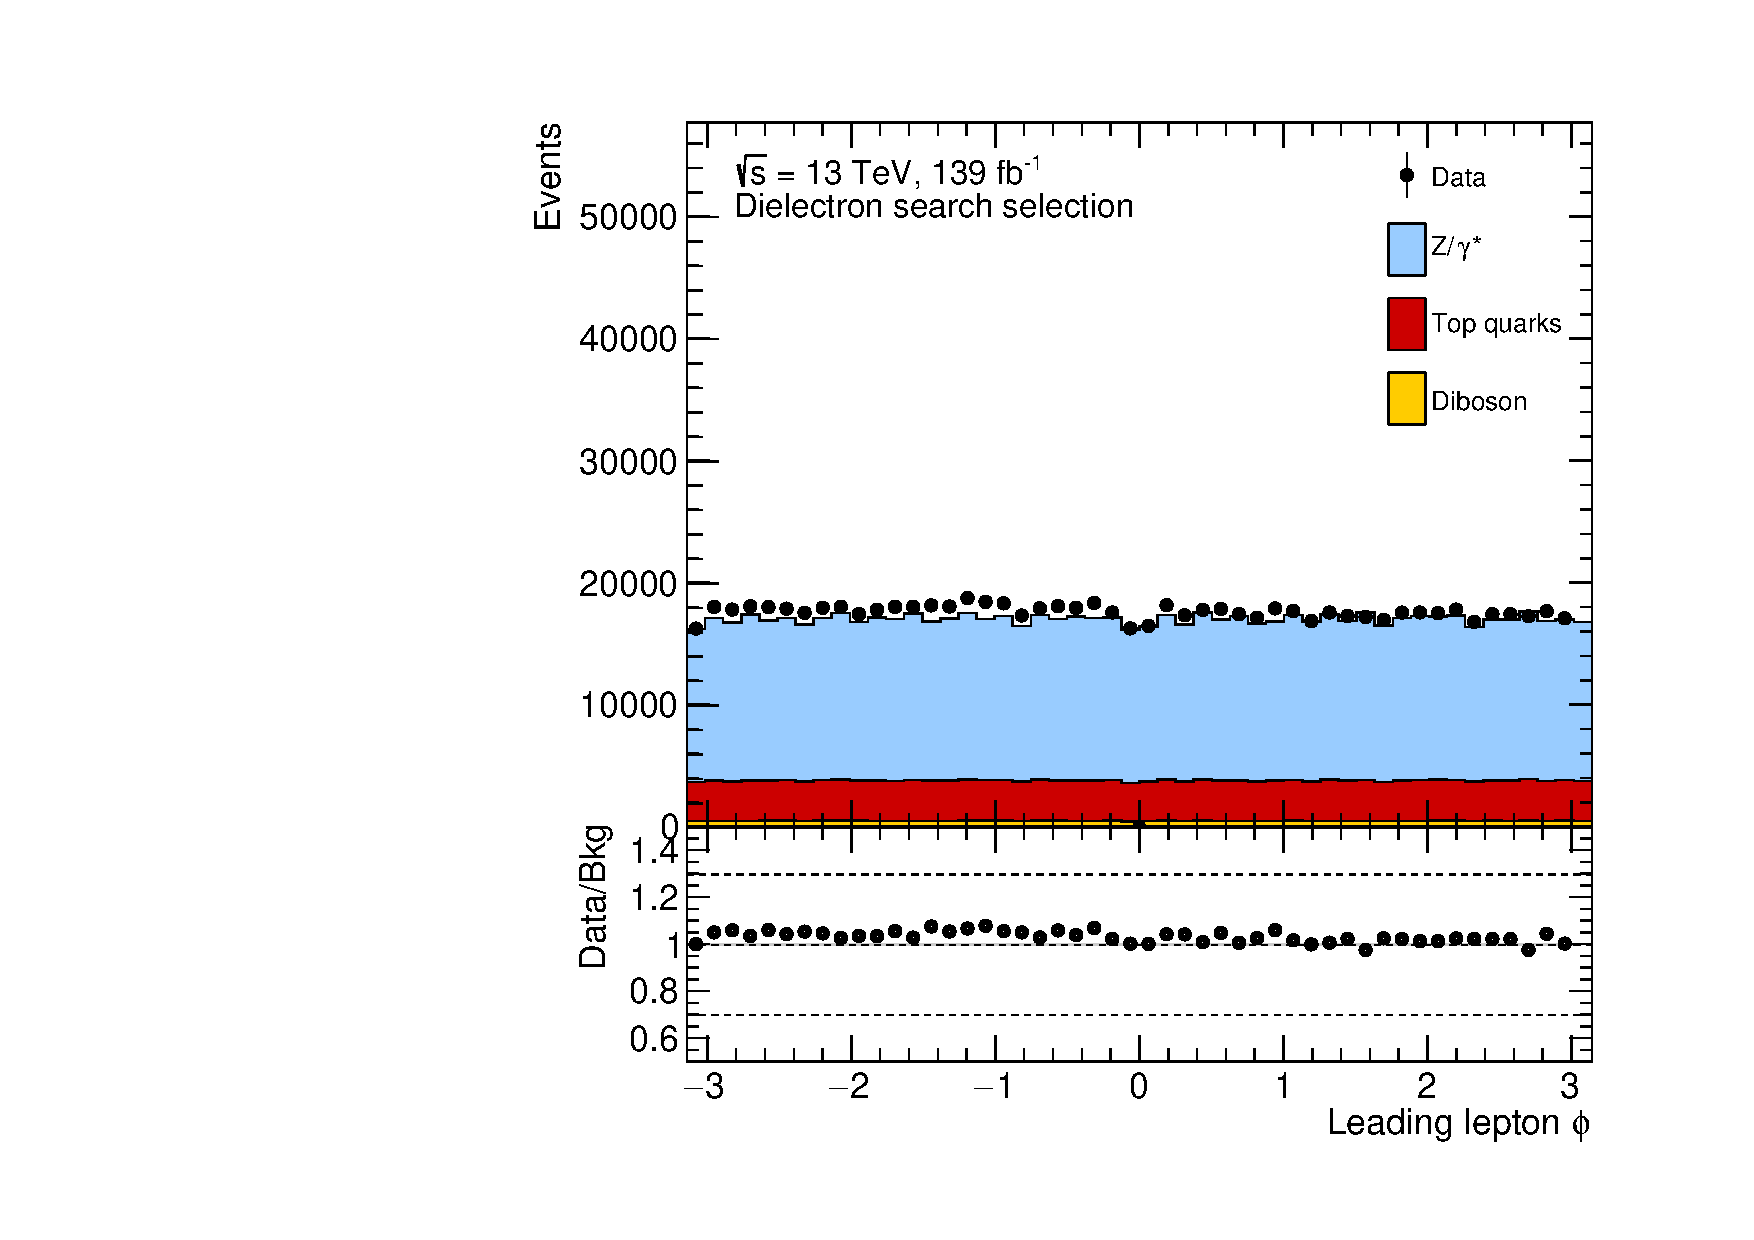
\includegraphics[width=\textwidth]{figures/analysis/datamc/dataMCcompare/ee_phi1.pdf}
        \label{fig:datamc:eephi1}
    \end{subfigure}
    \begin{subfigure}[b]{0.49\textwidth}
        \centering
        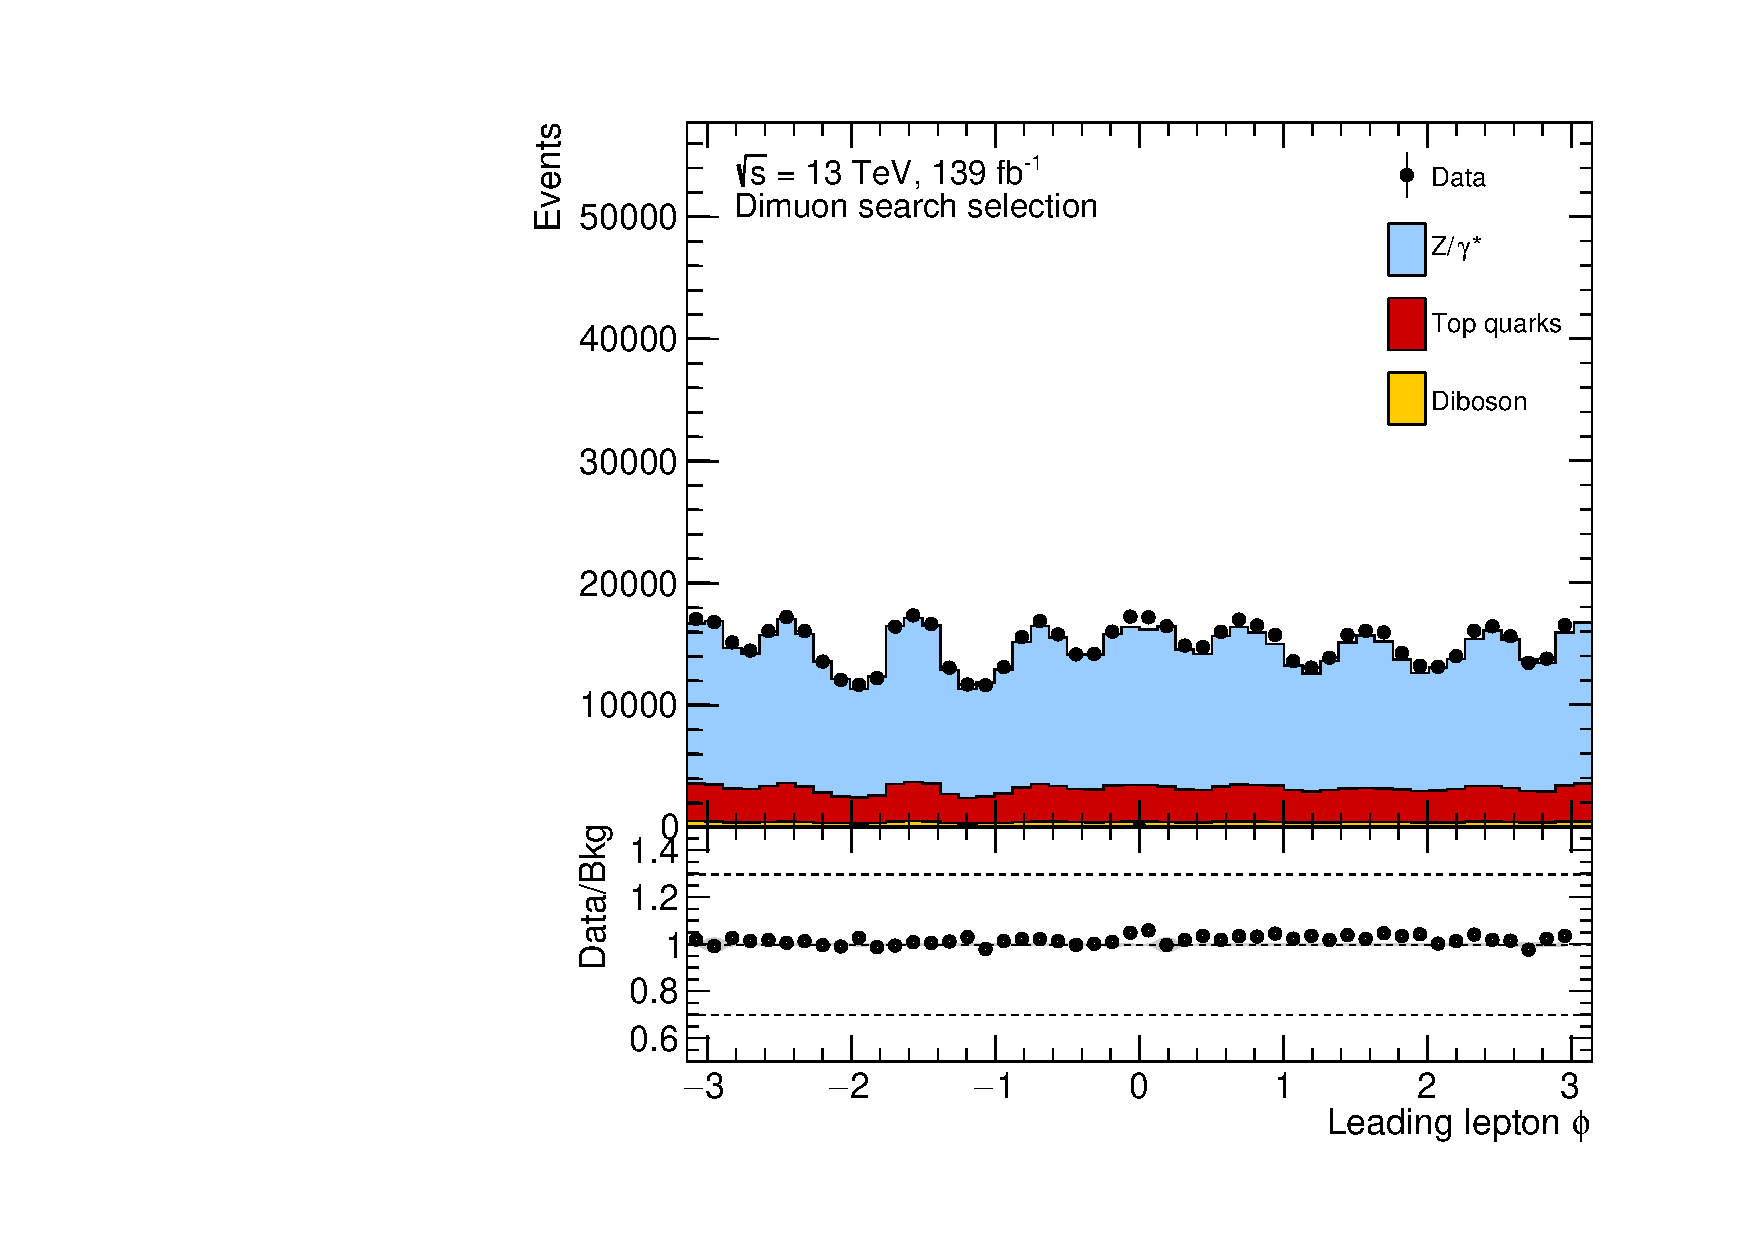
\includegraphics[width=\textwidth]{figures/analysis/datamc/dataMCcompare/uu_phi1.pdf}
        \label{fig:datamc:uuphi1}
    \end{subfigure}
    \caption[$\phi$ distribution of the leading lepton for the dilepton selections for the full $2015-18$ dataset and the respective MC campaigns.]{$\phi$ distribution of the leading lepton for the dilepton selections for the full $2015-18$ dataset and the respective MC campaigns. The \ee channel is shown in (left) and \mumu channel in (right). The bottom panel shows the ratio between the data and MC.}
    \label{fig:datamc:phi1}
\end{figure}

\begin{figure}[]
    \centering
    \begin{subfigure}[b]{0.49\textwidth}
        \centering
        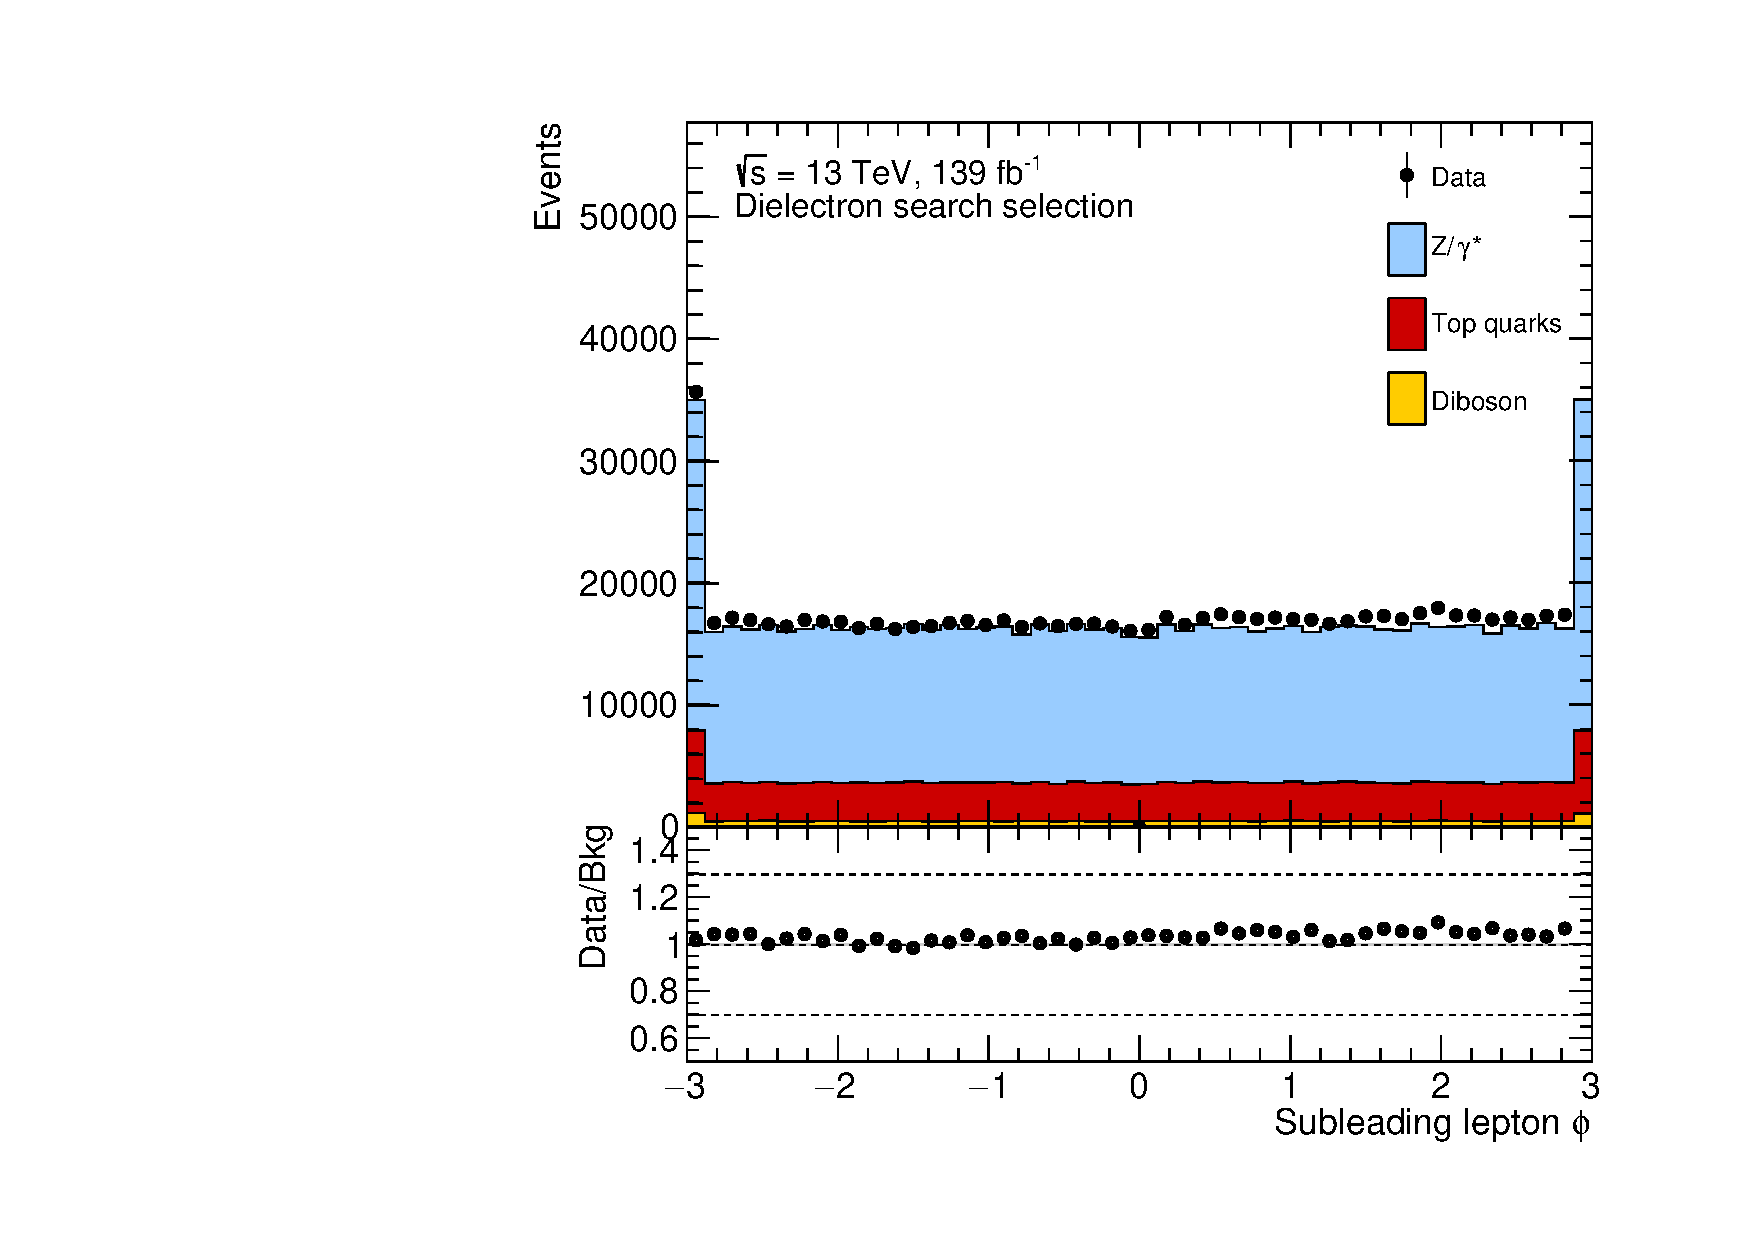
\includegraphics[width=\textwidth]{figures/analysis/datamc/dataMCcompare/ee_phi2.pdf}
        \label{fig:datamc:eephi2}
    \end{subfigure}
    \begin{subfigure}[b]{0.49\textwidth}
        \centering
        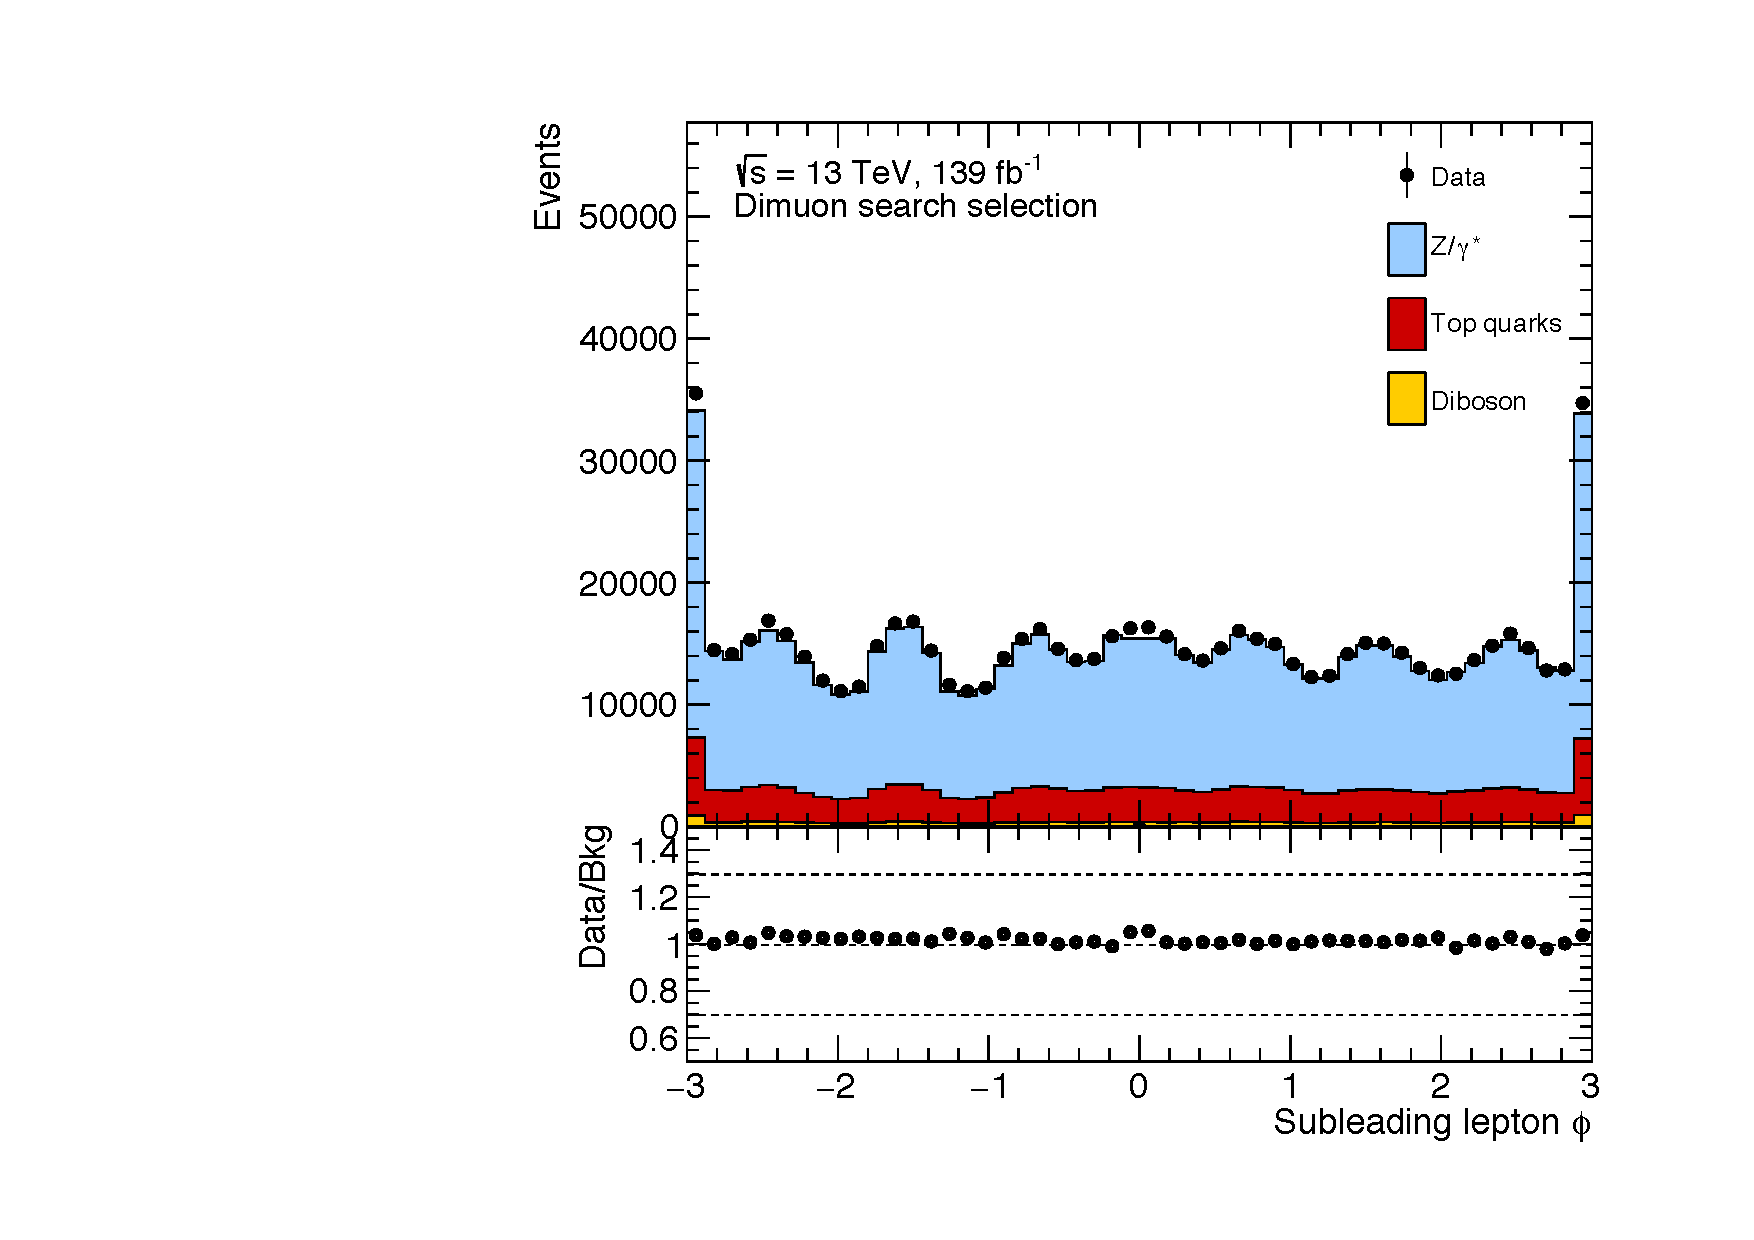
\includegraphics[width=\textwidth]{figures/analysis/datamc/dataMCcompare/uu_phi2.pdf}
        \label{fig:datamc:uuphi2}
    \end{subfigure}
    \caption[$\phi$ distribution of the subleading lepton for the dilepton selections for the full $2015-18$ dataset and the respective MC campaigns.]{$\phi$ distribution of the subleading lepton for the dilepton selections for the full $2015-18$ dataset and the respective MC campaigns. The \ee channel is shown in (left) and \mumu channel in (right). The bottom panel shows the ratio between the data and MC.}
    \label{fig:datamc:phi2}
\end{figure}

\clearpage